%%
%% This is file `gabaritTPA.tex',
%% generated with the docstrip utility.
%%
%% The original source files were:
%%
%% dms.dtx  (with options: `TPA,gabarit')
%% Example TeX file for the documentation
%% of the jurabib package
%% Copyright (C) 1999, 2000, 2001 Jens Berger
%% See dms.ins  for the copyright details.
%%
%%% ====================================================================
%%%  @LaTeX-file{
%%%     filename        = "dms.dtx",
%%%     author    = "Nicolas Beauchemin, Damien Rioux-Lavoie, Victor Fardel, Jonathan Godin",
%%%     copyright = "Copyright (C) 2000 , DMS
%%%                  all rights reserved.  Copying of this file is
%%%                  authorized only if either:
%%%                  (1) you make absolutely no changes to your copy,
%%%                  including name; OR
%%%                  (2) if you do make changes, you first rename it
%%%                  to some other name.",
%%%     address   = "Département de Mathématiques et de Statistique",
%%%     telephone = "514-343-6705",
%%%     FAX       = "514-343-5700",
%%%     email     = "aide@dms.umontreal.ca (Internet)",
%%%     keywords  = "latex, amslatex, ams-latex, theorem",
%%%     abstract  = " Ce fichier est un package conçu pour être
%%%                  utilisé avec la version de LaTeX2e 1995/06/01. Il
%%%                  est prévue pour la classe ``amsbook''. Il en
%%%                  modifie le format des pages, l'entête des
%%%                  sections, etc, afin d'être  conforme au modèle de
%%%                  mémoire de maîtrise de l'Université de
%%%                  Montréal. Finalement ce fichier est grandement
%%%                  inspiré du fichier amsclass.dtx.",
%%%     docstring = "The checksum field contains: CRC-16 checksum,
%%%                  word count, line count, and character count, as
%%%                  produced by Robert Solovay's checksum utility."}
%%%  ====================================================================

%% Pour voir les accents de ce fichier, assurez-vous que votre
%% éditeur de texte lise le fichier en utf-8!

%% La classe <dms> est construite au-dessus de <amsbook>, donc
%% <amsmath>, <amsfonts> et <amsthm> sont automatiquement chargés.
\documentclass[12pt,twoside,phd]{dms}
\usepackage[utf8]{inputenc} %Obligatoires
\usepackage[T1]{fontenc}    %

%% <lmodern> incorpore les fontes en T1, pour
%% faciliter le dépôt final. Ceci n'est pas la
%% seule option :
%%  1. Si cm-super est installé, vous pouvez enlever <lmodern>
%%     (à ce moment, la police est un peu plus fidèle
%%      au Computer Modern orginal);
%%  2. Si vous avez une police préférée, par exemple,
%%     <times> ou <euler> ou <mathpazo> (et bien d'autres),
%%     alors vous pouvez remplacer <lmodern> ci-bas.
%% Par contre, si vous faîtes face à un problème d'encapsulation
%% lors dépôt final, il se peut que la solution soit d'utiliser <lmodern>.
%% (Parfois le problème est au niveau de l'installation, donc
%%  essayez de compiler sur un autre ordinateur sur lequel vous êtes
%%  certain·e que l'installation est bonne.)
\usepackage{lmodern}

%% Il n'est pas nécessaire d'utiliser <babel>, car
%% les commandes intégrées par la classe <dms>
%% \francais et \anglais font le travail. Néanmoins,
%% certains autres packages nécessitent <babel> (comme
%% <natbib>), donc simplement enlever les % devant <babel>
%% dans ce cas. Attention! Certains packages sont sensibles
%% à l'ordre dans lequel ils sont chargés.
\francais % or
%%\anglais
%% KC added
\usepackage[english,frenchb]{babel}
\usepackage{natbib}
\usepackage{longtable}
\usepackage{tabularx}
\usepackage{booktabs}
\usepackage{afterpage}
\usepackage{floatpag}
\usepackage{float}
\floatplacement{figure}{H}
\usepackage{caption}
\usepackage{listings}
\providecommand{\tightlist}{%
  \setlength{\itemsep}{0pt}\setlength{\parskip}{0pt}}
\usepackage{lscape}
\newcommand{\blandscape}{\begin{landscape}}
\newcommand{\elandscape}{\end{landscape}}
\usepackage{makecell}
\usepackage{colortbl}
\usepackage{xcolor}

 % ENGLISH OPTION
 % If you call \anglais here before the \begin{document},
 % all the chater's header will be in english, even if you
 % call \francais. To change this, use
 % \entetedynamique

%% La commande \sloppy peut avoir des effets étranges sur les
%% lignes de certains paragraphes.  Dans ce cas, essayez \fussy
%% qui suppresse les effets de \sloppy.
%% (\fussy est normalement le comportement par défaut.)
%% On redéfinit \sloppy, pour tenter de réduire les comportements
%% étranges. Le seul changement apporté à la version originale
%% est la valeur de \tolerance.
\def\sloppy{%
  \tolerance 500%  %9999 dans LaTeX ordinaire, mauvaise idée.
  \emergencystretch 3em%
  \hfuzz .5pt
  \vfuzz\hfuzz}
\sloppy   %appel de \sloppy pour le document
%%\fussy  %ou \fussy

%% Packages utiles.
\usepackage{graphicx,amssymb,subfigure,icomma}
%% icomma       permet d'écrire les nombres décimaux en
%%                  français (p.ex. 1,23 plutôt que 1.23)
%% subfigure    simplifie l'inclusion de figures côtes-à-côtes

%% Packages parfois utiles.
%%\usepackage{dsfont,mathrsfs,color,url,verbatim,booktabs}
%% dsfont       symboles mathématiques \mathds
%% mathrsfs     plus de symboles mathématiques \mathscr
%% color        pour utiliser des couleurs (comparer avec <xcolor>)
%% url          permet l'écriture d'url
%% verbatim     pour écrire du code ou du texte tel quel
%% booktabs     plus de macros pour faire les tableaux
%%                  (voir documentation du package)

%% pour que la largeur de la légende des figures soit = \textwidth
\usepackage[labelfont=bf, width=\linewidth]{caption}

%% les 3 lignes suivante servent à l'affichage de l'index
%% dans le visionneur de pdf. <hyperref> et <bookmark>
%% devraient être les dernier package a être chargé,
%% donc chargez vos packages avant.
\usepackage{hyperref}  % Ajoute les hyperlien
\hypersetup{colorlinks=true,allcolors=black}
\usepackage{hypcap}   % Corrige la position du lien pour les images
\usepackage{bookmark} % Remédie à des petits problème
                      % de <hyperref> (important qu'il
                      % apparaisse APRÈS <hyperref>)

  % Enlever les commentaires du prochaine \hypersetup et
  % le remplir avec l'information pertinente.
  % Ceci ajoute des « méta-données » au pdf.  C'est optionnel,
  % mais recommandé. Vous pouvez voir ces méta-données en
  % ouvrant un visionneur de pdf et en cherchant les propriétés
  % du pdf. (Vous pouvez aussi tapez ' pdfinfo <nom-du-pdf> '
  % dans un terminal.) Ces données sont utiles, par exemple,
  % pour augmenter les chances qu'un algorithme de recherche
  % trouve votre document sur Internet, une fois diffusé.
  \hypersetup{
    pdftitle = {Dynamique spatio-temporelle des forêts dans l'écotone boréal-tempéré en réponse aux changements globaux},
    pdfauthor = {Marie-Hélène Brice},
    pdfsubject = {Dynamique forestière},
    pdfkeywords = {écologie des communautés, changements climatiques, forêts, diversité bêta, dynamique de transition, recrutement, Québec}
  }

%% Définition des environnements utiles pour un mémoire scientifique.
%% La numérotation est laissée à la discrétion de l'auteur·e. L'exemple
%% illustré ici produit « Définition x.y.z » à l'extérieur d'un article
%%   x = no. chapitre
%%   y = no. section
%%   z = no. définition
%% et « Définition x » à l'intérieur d'un article
%%   x = no. définition
%% Les numérotations des corollaires, définitions, etc.
%% se font de façon successive.
%%
%% Les macros \<type>name sont telles qu'ils suivent
%% la langue actuelle. (P.ex. si \francais est utilisé,
%% alors \begin{theo} va faire un Théorème et si \anglais
%% est utilisé, \begin{theorem} fera un Theorem.)
%%
  % Environnement à utiliser à l'extérieur des articles
\newtheorem{cor}{\corollaryname}[section]
\newtheorem{deff}[cor]{\definitionname}
\newtheorem{ex}[cor]{\examplename}
\newtheorem{lem}[cor]{\lemmaname}
\newtheorem{prop}[cor]{Proposition}
\newtheorem{rem}[cor]{\remarkname}
\newtheorem{theo}[cor]{\theoremname}

  % Environnement à utiliser à l'intérieur des articles
\newtheorem{corA}{\corollaryname}
\newtheorem{deffA}[corA]{\definitionname}
\newtheorem{exA}  [corA]{\examplename}
\newtheorem{lemA} [corA]{\lemmaname}
\newtheorem{propA}[corA]{Proposition}
\newtheorem{remA} [corA]{\remarkname}
\newtheorem{theoA}[corA]{\theoremname}
%% IMPORTANT : Il faut faire \setcounter{corA}{0}
%% au début d'un article pour recommancer à compter à 1.
%%
%% NOTE : Il peut être commode de redéfinir \the<type> pour
%% obtenir la numérotation désirée. Par exemple, pour
%% que les corollaires soit numérotés #article.#section.#sous-section,
%% on fait
%% \renewcommand\thecorA{\thepart.\thesubsection.\arabic{corA}}

%%%
%%% Si vous préférez que les corollaires, définitions, théorèmes,
%%% etc. soient numérotés séparément, utilisez plutôt un bloc de
%%% commandes de la forme :
%%%

%%\newtheorem{cor}{\corollaryname}[section]
%%\newtheorem{deff}{\definitionname}[section]
%%\newtheorem{ex}{\examplename}[section]
%%\newtheorem{lem}{\lemmaname}[section]
%%\newtheorem{prop}{Proposition}[section]
%%\newtheorem{rem}{\remarkname}[section]
%%\newtheorem{theo}{\theoremname}[section]

%%
%% Numérotation des équations par section
%% et des  tableaux et figures par chapitre.
%% Ceci peut être modifié selon les préférences de l'utilisateur.
\numberwithin{equation}{section}
\numberwithin{table}{chapter}
\numberwithin{figure}{chapter}

%%
%% Si on veut faire un index, il faut décommenter la ligne
%% suivante. Ajouter des mots à l'index avec la commande \index{mot cle} au
%% fur et à mesure dans le texte.  Compiler, puis taper la commande
%% makeindex pour creer les indexs.  Après une nouvelle compilation,
%% vous aurez votre index.
%%

%%\makeindex

%% Il est obligatoire d'écrire à double interligne
%% ou à interligne et demi. On peut soit utiliser
%% le package <setspace> ou \baselinestretch.
%% Le package est un peu plus propre, mais le choix
%% reste à la discrétion de l'usager.
\usepackage[onehalfspacing]{setspace}
 % ou
%%\renewcommand{\baselinestretch}{1.5}


%%%%%%%%%%%%%%%%%%%%%%%%%%%%%%%%%%%%%%%%%%%%%%%%%%%%%%%%%%%%
%%%%%%%%%%%%%%%%%%%%%%%%%%%%%%%%%%%%%%%%%%%%%%%%%%%%%%%%%%%%
%%%%%%%%%%                                     %%%%%%%%%%%%%
%%%%%%%%%% D é b u t    d u    d o c u m e n t %%%%%%%%%%%%%
%%%%%%%%%%                                     %%%%%%%%%%%%%
%%%%%%%%%%%%%%%%%%%%%%%%%%%%%%%%%%%%%%%%%%%%%%%%%%%%%%%%%%%%
%%%%%%%%%%%%%%%%%%%%%%%%%%%%%%%%%%%%%%%%%%%%%%%%%%%%%%%%%%%%
\begin{document}

%%
%% Voici des options pour annoter les différentes versions de votre
%% mémoire. La commande \brouillon imprime, au bas de chacune des pages, la
%% date ainsi que l'heure de la dernière compilation de votre fichier.
%%
%%\brouillon
%%
%%
%% \version est la version de votre manuscrit
%%
\version{1}

%%------------------------------------------------- %
%%              pages i et ii                       %
%%------------------------------------------------- %

%%%
%%% Voici les variables à définir pour les deux premières pages de votre
%%% mémoire.
%%%

\title{Dynamique spatio-temporelle des forêts dans l'écotone boréal-tempéré en réponse aux changements globaux}

\author{Marie-Hélène Brice}

\copyrightyear{2020}

\department{Département de sciences biologiques}

\date{\today} %Date du DÉPÔT INITIAL (ou du 2e dépôt s'il y a corrections majeures)

\sujet{sciences biologiques}
\orientation{option biodiversité, écologie et évolution}%Ce champ est optionnel
%%\orientation{orientation}%Ce champ est optionnel
%%
%% Voici les disciplines possibles (voir avec votre directeur):
%% \sujet{statistique},
%% \sujet{mathématiques}, \orientation{mathématiques appliquées},
%% \orientation{mathématiques fondamentales}
%% \orientation{mathématiques de l'ingénieur} et
%% \orientation{mathématiques appliquées}

\president{Pierre-Luc Chagnon}

\directeur{Pierre Legendre}

\codirecteur{Marie-Josée Fortin}

\membrejury{Steven Kembel}

\examinateur{Sylvie de Blois}

%%\codirecteur{Nom du 1er codirecteur}         % s'il y a lieu
%%\codirecteurs{Nom du 2e codirecteur}         % s'il y a lieu


%%\examinateur{Nom de l'examinateur externe}   %obligatoire pour la these

%% \membresjury{Deuxième membre du jury}  % s'il y a lieu

%%  \plusmembresjury{Troisième membre du jury}    % s'il y a lieu

 % Cette option existe encore, mais elle n'a plus sa place
 % dans la page titre. L'utiliser seulement si le directeur
 % insiste...
%%\repdoyen{Nom du représentant du doyen} %(thèse seulement)

%%
%% La commande \maketitle créera votre page titre.

\maketitle

 % Pour générer la deuxième page titre, il faut appeler à nouveau \maketitle
 % Cette page est obligatoire.
\maketitle

%%------------------------------------------------- %
%%              pages iii                           %
%%------------------------------------------------- %

 % Les articles peuvent être en anglais, mais
 % les autres parties du document doivent être
 % en français. Il faut une permission pour
 % écrire l'ensemble de la thèse en anglais.
 % Consulter le guide de présentation des mémoires
 % et des thèses pour de l'information plus
 % précise et à jour.
\francais

\chapter*{Résumé}

...sommaire et mots clés en français...

%%------------------------------------------------- %
%%              pages iv                            %
%%------------------------------------------------- %

\anglais
\chapter*{Abstract}

...summary and keywords in english...

%%------------------------------------------------- %
%%        page v --- Table de matieres              %
%%------------------------------------------------- %

\francais
 % \cleardoublepage termine la page actuel et force TeX
 % a poussé les éléments flottant (fig., tables, etc.) sur
 % la page (normalement TeX les garde en suspend jusqu'à ce
 % qu'il trouve un endroit approprié). Avec l'option <twoside>,
 % la commande s'assure que la prochaine page de texte est sur
 % le recto, pour l'impression. On l'utilise ici
 % pour que TeX sache que la table des matières etc. soit
 % sur la page qui suit.
%% TABLE DES MATIÈRES
\cleardoublepage
\pdfbookmark[chapter]{\contentsname}{toc}  % Crée un bouton sur
                                           % la bar de navigation
\tableofcontents
 % LISTE DES TABLES
\cleardoublepage
\phantomsection  % Crée une section invisible (utile pour les hyperliens)
\listoftables
 % LISTE DES FIGURES
\cleardoublepage
\phantomsection
\listoffigures

%%%%%%%%%%%%%%%%%%%%%%%%%%%%%%%%%%%%%
%% LISTE DES SIGLES ET ABRÉVIATION %
%%%%%%%%%%%%%%%%%%%%%%%%%%%%%%%%%%%%%
%% Il est obligatoire, selon les directives de la FESP,
%% pour une thèse ou un mémoire d'avoir une liste des sigles et
%% des abréviations.  Si vous considérez que de telles listes ne seraient pas
%% pertinentes (si, par exemple, vous n'utilisez aucun sigle ou abré.), son
%% inclusion ou omission est laissé à votre discrétion.  En cas de doute,
%% parlez-en à votre directeur de recherche, le coadministrateur ou au/à la
%% bibliothécaire.
%%
%% Le gabarit inclut un exemple d'une liste « fait à la main ».  Il existe des outils
%% plus sophistiqués si vous devez inclure une multitude de sigles et abréviations.
%% Par exemple, le package <glossaries> peut faire des index élaborés.  Comme
%% son utilisation est technique, il n'y a pas d'exemple directement dans ce gabarit.
%% On invite les gens qui aurait à l'utiliser à lire la documentation officielle,
%% soit en allant sur https://www.ctan.org/, soit en tapant dans un terminal :
%%
%% texdoc glossaries
%%

\chapter*{Liste des sigles et des abréviations}
 % Option de colonnes: definir \colun ou \coldeux
%%% Exemple
%%% \def\colun{\bf} % Première colonne en gras
%%% Pour numéroté les entrées, on peut faire
%%% \newcount\abbrlist
%%% \abbrlist=0
%%% \def\plusun{\global\advance\abbrlist by 1\relax}
%%% \def\colun{\plusun\the\abbrlist. }
%%\def\coldeux{\relax}
\begin{twocolumnlist}{.2\textwidth}{.7\textwidth}
  AIC & Critère d'information d'Akaike, de l'anglais \textit{Akaikes Information Criteria}\\
  DBH  & Diamètre hauteur poitrine (1.3m), de l'anglais
      \textit{Diameter at breast height} \\
  CTI  &  Indice de température de la communauté, de l'anglais
    \textit{Community  Temperature Index}\\
  GES & Gaz à effet de serre\\
  GIEC & Groupe d'experts intergouvernemental sur l'évolution du climat\\
  PCA & Analyse en composantes principales, de l'anglais \textit{Principal component Analysis}\\
  sd & Écart standard, de l'anglais \textit{standard deviation}\\
  SDM  &  Modèle de distribution des espèces, de l'anglais \textit{Species Distribution Model}\\
  STI  &  Indice de température des espèces, de l'anglais \textit{Species Temperature Index}\\
  TBI  &  Indice de diversité beta temporelle, de l'anglais \textit{Temporal Beta diversity Index}\\
\end{twocolumnlist}
%% L'environnement <threecolumnlist> existe aussi pour trois colonnes.

%%------------------------------------------------- %
%%              pages vi                            %
%%------------------------------------------------- %

\chapter*{Remerciements}

...remerciements...

 %
 % Fin des pages liminaires.  À partir d'ici, les
 % premières pages des chapitres ne doivent pas
 % être numérotées
 %

\NoChapterPageNumber
\cleardoublepage




%%%%%%%%%%%%%%%%%%%%%%%%%%%%%%%%%%%%%%%%%%%%%%%%%%%%%%%%%%%%
%%%%%%%%%%%%%%%%                           %%%%%%%%%%%%%%%%%
%%%%%%%%%%%%%%%%  I N T R O D U C T I O N  %%%%%%%%%%%%%%%%%
%%%%%%%%%%%%%%%%                           %%%%%%%%%%%%%%%%%
%%%%%%%%%%%%%%%%%%%%%%%%%%%%%%%%%%%%%%%%%%%%%%%%%%%%%%%%%%%%

\renewcommand\thefigure{0.\arabic{figure}}
\renewcommand\thetable{0.\arabic{table}}

\francais
\chapter*{Introduction}

\hypertarget{introduction-guxe9nuxe9rale}{%
\section{Introduction générale}\label{introduction-guxe9nuxe9rale}}

L'humain est aujourd'hui une force prédominante gouvernant les processus
écologiques, amenant de nombreux chercheurs à suggérer que le système
terrestre a basculé dans une nouvelle ère géologique, l'Anthropocène
\citep{crutzen_geology_2002}. Depuis environ un siècle, les activités
humaines ont largement perturbé l'équilibre dynamique des cycles
naturels. Le développement des sociétés occidentales s'est basé sur
l'industrialisation et l'exploitation des ressources, résultant
notamment en un changement d'utilisation des sols associé à la
fragmentation et la dégradation des habitats, ainsi qu'à un relargage
massif de gaz à effet de serre (e.g.~CO2, SOx, CH4, NOx\ldots) dans
l'atmosphère. Les changements environnementaux récents se caractérisent
par leur vitesse et leur intensité. La recherche scientifique
contemporaine s'intéresse à comprendre, évaluer et prédire l'impact de
ces perturbations sur les écosystèmes et les communautés (McGill et al.,
2015; Root et al., 2003; Sala et al., 2000; Vellend et al., 2017).

\hypertarget{changements-climatiques}{%
\section{Changements climatiques}\label{changements-climatiques}}

Le réchauffement climatique mesuré sur l'ensemble de la planète durant
les dernières décennies est sans équivoque, et la responsabilité de
l'humain par l'émission de gaz à effet de serre (abrégé GES par la
suite) est clairement établie \citep{ipcc_climate_2014}. Des projections
récentes des changements climatiques indiquent que les températures
moyennes mondiales pourraient augmenter de 2.6 à 4.8\(^{\circ}\)C d'ici
la fin du XXIe siècle dans le nord-est de l'Amérique du Nord, s'il n'y a
pas de progrès sur le contrôle des émissions de GES anthropiques
\citep{ipcc_climate_2014}. Le climat étant un déterminant important de
la distribution des espèces, de telles augmentations de température
auront un impact majeur sur la structure et les fonctions de tous les
écosystèmes \citep{bellard_impacts_2012, gauthier_vulnerability_2015}.

Selon les prévisions, les changements de température et de régimes de
précipitation devraient déplacer les niches climatiques optimales de
nombreuses espèces d'arbres vers le nord sur des centaines de kilomètres
\citep{mckenney_potential_2007} ou plus haut en altitude d'une centaine
de mètres \citep{jump_altitude-for-latitude_2009}, modifiant la
composition, la structure et la diversité forestières
\citep{price_anticipating_2013, reich_geographic_2015}. Or, de tels
changements dans les forêts peuvent avoir des répercussions
environnementales considérables sur les fonctions et les services des
écosystèmes, tels que l'approvisionnement en bois et en produits
forestiers non ligneux, le stockage du carbone, le cycle des nutriments,
la purification de l'air et de l'eau et le maintien d'habitats pour la
faune et la flore \citep{mitchell_linking_2013, mori_biodiversity_2017}.
Ces changements soulèvent aussi des enjeux socio-économiques majeurs.
Par exemple, comment adapter les stratégies de gestion forestière pour
assurer un approvisionnement durable en bois ? Ou encore, quel est
l'avenir de certaines espèces économiquement et culturellement
importantes, comme l'érable à sucre au Québec ? Comprendre et prédire
les conséquences de ces changements climatiques sur les écosystèmes
forestiers représente donc l'un des grands défis actuels pour la
communauté scientifique
\citep{pereira_scenarios_2010, garcia_multiple_2014}.

\hypertarget{ruxe9ponses-des-uxe9cosystuxe8mes-forestiers-aux-changements-climatiques}{%
\section{Réponses des écosystèmes forestiers aux changements
climatiques}\label{ruxe9ponses-des-uxe9cosystuxe8mes-forestiers-aux-changements-climatiques}}

\hypertarget{duxe9placements-des-aires-de-ruxe9partition}{%
\subsection{Déplacements des aires de
répartition}\label{duxe9placements-des-aires-de-ruxe9partition}}

Des changements de distribution liés au climat ont déjà été observés
pour de nombreuses espèces d'arbres à différentes échelles spatiales,
particulièrement dans les zones de transition où les changements sont
plus facilement détectables
\citep{jump_altitude-for-latitude_2009, boulanger_climate_2017}. Par
exemple, à l'échelle locale, \citet{fisichelli_temperate_2014} ont
observé une avancée de la régénération d'espèces arbres tempérées dans
la forêt boréale de la région à l'ouest des Grands Lacs et ce processus
semblait être facilité par des températures plus chaudes.
\citet{leithead_northward_2010} ont observé que les trouées causées par
la mort des arbres boréaux dans une forêt du nord de l'Ontario
facilitent l'établissement d'espèces tempérées du sud. Les changements
dans la composition forestière ont aussi été observés dans les écotones
altitudinaux sur une période de 40 ans; dans les Montagnes Vertes du
Vermont, les arbres tempérés ont progressé en altitude, conduisant à un
déplacement des limites de l'écotone boréal-tempéré d'environ 100 m
\citep{beckage_rapid_2008}, tandis que sur le Mont-Mégantic au sud du
Québec, les arbres se sont déplacés en élévation de près de 30 m en
moyenne et les espèces de sous-bois de près de 40 m
\citep{savage_elevational_2015}. Mis ensemble, ces derniers résultats
indiquent qu'un décalage dans la répartition des deux strates de
végétation, et donc un changement de composition, est déjà en train de
se former dû à une différence entre la vitesse de réponse des espèces de
sous-bois et celle des arbres. À l'échelle régionale,
\citet{boisvert-marsh_shifting_2014} et \citet{sittaro_tree_2017} ont
montré une migration à prédominance vers le nord des essences d'arbres à
travers le Québec, avec les gaulis présentant une réponse plus rapide
que les arbres adultes.

\hypertarget{ruxe9ponses-duxe9mographiques}{%
\subsection{Réponses
démographiques}\label{ruxe9ponses-duxe9mographiques}}

Alors que de nombreuses études sur l'impact des changements climatiques
sur les forêts ont tenté de détecter ou de prédire les déplacements des
limites d'aires de répartition des espèces, comparativement peu d'études
ont examiné les changements à long terme des taux démographiques,
e.g.~mortalité, recrutement, croissance, ou ont exploré les facteurs
environnementaux responsables de ces changements \citep[reviewed
in][]{allen_global_2010}. L'accent mis sur les déplacements des espèces
vers les pôles sous-estime l'empreinte des changements climatiques. Les
changements de température et de précipitations ont des effets directs
sur la croissance, la mortalité et le recrutement des arbres
\citep{vanderwel_climate-related_2013, zhang_half-century_2015}. Par
exemple, les augmentations récentes des taux de mortalité des arbres
dans l'ouest de l'Amérique du Nord ont été attribuées à des températures
élevées et des sécheresses
\citep{van_mantgem_widespread_2009, peng_drought-induced_2011}. Or,
c'est l'équilibre entre les gains par la croissance et le recrutement et
les pertes par la mortalité qui détermine, localement, la dynamique des
forêts et, régionalement, les limites d'aires de répartition
\citep{holt_theoretical_2005}. Des changements même très faibles dans
les taux démographiques peuvent modifier le rapport de force de la
compétition interspécifique
\citep{luo_observations_2013, reich_geographic_2015}, de même que la
dynamique et la trajectoire de succession des forêts
\citep{prach_four_2011}, modifiant par conséquent leur structure et leur
composition \citep{van_mantgem_widespread_2009, stephenson_causes_2011}.
À long terme, ces changements démographiques agissent donc pour
contrôler les limites géographiques des différents types de forêts
\citep{holt_theoretical_2005}.

Étant donné l'échelle temporelle à laquelle les changements de
répartition se produisent pour des organismes à longue durée de vie
comme les arbres, comprendre l'influence des conditions abiotiques et
biotiques sur les taux démographiques des populations offre une
meilleure perspective sur la biogéographie des espèces et permet
d'inférer les changements continus à la limite et à l'intérieur de
l'aire de répartition
\citep{sexton_evolution_2009, schurr_how_2012, thuiller_road_2013, snell_using_2014}.
Pourtant, à l'heure actuelle, il existe très peu d'informations
quantitatives sur l'effet combiné des changements climatiques et des
multiples perturbations forestières sur ces processus fondamentaux de la
dynamique forestière.

\hypertarget{duxe9lais-de-ruxe9ponse-et-duxe9suxe9quilibre}{%
\section{Délais de réponse et
déséquilibre}\label{duxe9lais-de-ruxe9ponse-et-duxe9suxe9quilibre}}

Bien qu'on prévoie un déplacement des niches climatiques des arbres de
plusieurs centaines de kilomètres vers le nord d'ici la fin du siècle
\citep{mckenney_potential_2007}, un nombre croissant d'études suggèrent
que le déplacement des arbres en Amérique du Nord ne réussira
probablement pas à suivre le rythme du réchauffement climatique
\citep{zhu_failure_2012, woodall_assessing_2013, vissault_biogeographie_2016, sittaro_tree_2017}.
Par exemple, malgré qu'on observe un déplacement des aires de
répartition des arbres vers le nord, les vitesses de migration des
espèces d'arbres au Québec étaient en moyenne inférieures à 50\% de la
vitesse d'avancée géographique des changements climatiques récents
\citep{sittaro_tree_2017}.

Les arbres sont particulièrement susceptibles de montrer de longs délais
de réponse aux changements parce que ces espèces sont sessiles, ont une
faible capacité de dispersion, une longue durée de vie, une croissance
lente et une maturité sexuelle tardive
\citep{iverson_tree-species_2013, lenoir_climate-related_2015}. Ces
caractéristiques pourraient expliquer le haut niveau d'inertie des
forêts malgré les changements de climat
\citep{vissault_biogeographie_2016}. En effet, ces caractéristiques
peuvent expliquer l'absence de colonisation à la limite nord malgré que
les conditions soient devenues favorables et engendrer un crédit de
colonisation. Inversement, les espèces peuvent persister pendant un
certain temps dans un milieu nouvellement inadapté en raison du délai
d'extinction ou peuvent être maintenues grâce à une dynamique
source-puit, engendrant une dette d'extinction
\citep{pulliam_relationship_2000, jackson_balancing_2010, schurr_how_2012}.
Ainsi, étant donné que l'environnement est dynamique et que les
écosystèmes forestiers sont caractérisés par d'importants délais de
colonisation et d'extinction, les systèmes perturbés ne parviennent
souvent pas à un équilibre statistique sur des échelles temporelles et
spatiales réalistes pour permettre une analyse statique (e.g., SDM). Il
y a donc un décalage entre la niche Hutchinsonienne et la répartition
géographique d'une espèce \citep{holt_bringing_2009}. Pourtant, la
majorité des modèles de distribution d'espèces suppose que les espèces
sont en équilibre avec leur environnement, ignorant la dynamique de
transition.

D'importants délais de réponse des forêts aux changements climatiques
sont déjà observables puisque la distribution de plusieurs espèces
d'arbres de l'est de l'Amérique du Nord n'est pas à l'équilibre avec le
climat aux marges de leur aire de répartition, avec davantage de dettes
d'extinction au sud et de crédits de colonisation au nord
\citep{talluto_extinction_2017}. Leurs résultats montrent aussi que la
vitesse de la contraction d'aire de répartition dans le sud est plus
rapide que l'expansion dans le nord \citep{talluto_extinction_2017}).
Des simulations ont aussi montré que le décalage entre la niche
climatique optimale des espèces tempérées et leur distribution réalisée
ne fera que s'accroître avec le temps
\citep{vissault_biogeographie_2016}. Cette tension grandissante entre la
distribution réalisée et potentielle des espèces risque d'autant plus de
causer des changements brusques (regime shift) dans les écosystèmes
forestiers suite à une perturbation anthropique ou naturelle
\citep{vanderwel_how_2014, renwick_temporal_2015}.

\hypertarget{contraintes-uxe0-la-migration}{%
\section{Contraintes à la
migration}\label{contraintes-uxe0-la-migration}}

\hypertarget{interactions-biotiques}{%
\subsection{Interactions biotiques}\label{interactions-biotiques}}

Alors que le climat est un déterminant majeur de la niche des espèces,
des facteurs non climatiques, tels que les interactions biotiques,
imposent des contraintes supplémentaires à la migration des espèces.
Bien qu'elles répondent de manière indépendante, les espèces ne sont pas
isolées, mais interagissent avec les membres de leur communauté. Il est
généralement admis que les facteurs déterminant la distribution sont
spatialement hiérarchisés, de sorte que le climat régirait la
répartition à l'échelle régionale, alors que les interactions biotiques
seraient plus importantes à l'échelle locale
\citep{soberon_grinnellian_2007}. De plus, le climat contraindrait la
distribution et l'abondance des espèces à leur limite nord, tandis que
le rôle des interactions serait plus important à la limite sud et à
l'intérieur de l'aire de répartition, là où les conditions
environnementales sont plus favorables \citep{louthan_where_2015}. Un
bon exemple de ce phénomène est la distribution de l'épinette noire, une
espèce ayant une niche écologique très large, mais dont la distribution
au sud est limitée aux sites où la compétition est faible
\textbf{(Loehle 1998)}, comme des sites à drainage très mauvais ou
excessif. Toutefois, avec les changements climatiques, les conditions
favorables se déplacent et forcent de nouvelles interactions à la marge
des aires de distributions \citep{kissling_multispecies_2015}. Par
exemple, à moins qu'un dépérissement massif de la forêt ne se produise,
les espèces tempérées qui migreront dans les forêts boréales devront
s'établir sur des sites qui sont déjà colonisés par d'autres espèces et
devront donc vraisemblablement compétitionner pour les ressources lors
de leur établissement \citep[phénomène appelé l'effet
prioritaire;][]{gilman_framework_2010}. Plus la compétition par les
espèces résidentes sera forte, plus la probabilité de colonisation par
les espèces migratrices diminuera, car ces dernières parviendront
difficilement à s'installer \citep{cazelles_integration_2016}, d'où
l'importance potentielle des interactions dans la distribution à grande
échelle. Une étude de simulation a d'ailleurs révélé que les taux de
migration sont plus faibles dans les forêts établies que dans les forêts
de début de succession, et lorsque la diversité est grande
\citep{meier_climate_2012}. Ainsi, les espèces de début de succession
ont des taux de migration plus rapides que les espèces de fin de
succession puisque ces dernières colonisent principalement les habitats
forestiers déjà colonisés où la compétition interspécifique est plus
élevée \citet{meier_climate_2012}{]}. Les interactions biotiques sont de
plus en plus reconnues comme étant un facteur clé influençant la
distribution des espèces à grande échelle
\citep{meier_biotic_2010, blois_climate_2013, wisz_role_2013, svenning_influence_2014, cazelles_theory_2016}.

Comme la répartition géographique d'une espèce dépend de nombreux
facteurs environnementaux, ainsi que des limites de dispersion et des
contingences historiques
\citep{pulliam_relationship_2000, holt_bringing_2009, godsoe_i_2010}, il
peut s'avérer difficile sur le plan technique de trouver des preuves de
l'effet des interactions entre espèces sur la distribution. Les limites
physiologiques des espèces (et donc l'hétérogénéité environnementale)
influencent les interactions biotiques puisqu'elles déterminent le pool
d'espèces qui peuvent potentiellement cohabiter à un endroit donné. Les
patrons de cooccurrence des espèces en compétition sont en partie dus au
hasard, déterminés par qui est arrivé le premier et par des facteurs
aléatoires qui donnent un avantage initial. L'influence de l'effet
prioritaire et de l'hétérogénéité environnementale sur la répartition
actuelle des espèces rend donc difficile l'estimation de la force de
compétition à partir des patrons de cooccurrence ; une faible
cooccurrence peut refléter une faible compétition actuelle, mais une
forte compétition dans le passé, et inversement une forte cooccurrence
peut indiquer une faible compétition puisque les espèces coexistent,
mais aussi une forte compétition pour les mêmes ressources.

Bien que plusieurs études sur les déplacements d'aires de répartition
soulignent que les interactions biotiques risquent de réduire le succès
de migration, les preuves empiriques de leurs impacts sur les taux de
migration sont rares et indirectes \citep{svenning_influence_2014}. Les
interactions interspécifiques représentent donc un facteur inconnu clé
dans les études sur le changement climatique. Une étude approfondie des
taux de recrutements et de mortalités pourrait permettre de tester et
quantifier l'importance du rôle joué par les interactions biotiques sur
la dynamique de transition et de migration des arbres.

\hypertarget{propriuxe9tuxe9s-du-sol}{%
\subsection{Propriétés du sol}\label{propriuxe9tuxe9s-du-sol}}

En plus de la compétition interspécifique, les espèces migratrices
coloniseront des sols qui sont déjà développés et qui présentent des
propriétés (e.g.~qualité du drainage, disponibilité en nutriments, pH,
mycorhizes) qui varient localement ou régionalement, lesquelles
pourraient retarder ou contraindre leur établissement
\citep{goldblum_deciduous_2010, lafleur_response_2010, brown_non-climatic_2014}.
Les forêts dominées par les conifères au nord où la température moyenne
est froide présentent généralement des sols plus acides et conduisent à
une activité microbienne plus faible et à une décomposition plus lente
de la matière organique que les forêts tempérées décidues plus chaudes
du sud \citep{goldblum_deciduous_2010}. Par exemple,
\citet{collin_conifer_2017} ont montré que l'acidité du sol forestier
sous une canopée dominée par les conifères affecte négativement les
semis de l'érable à sucre via un débalancement nutritif foliaire, ce qui
pourrait donc freiner sa migration dans la forêt boréale. Toutefois, les
espèces forestières, par leur effet sur la qualité chimique de la
litière (C, N, Mg) et sur la composition des microorganismes du sol,
peuvent elles-mêmes modifier les taux de décomposition de la matière
organique et la disponibilité des éléments nutritifs
\citep{laganiere_how_2010}. Les espèces migratrices pourraient donc
influencer leur propre taux d'invasion. Plusieurs études menées dans le
nord-est du Canada ont montré une colonisation rapide des peuplements
résineux par le peuplier faux-tremble après une perturbation par la
coupe forestière ou les feux
\citep{chen_wildfire_2009, laquerre_augmentation_2009}. La présence de
cette espèce décidue induit des changements physicochimiques et accélère
les taux de décomposition de la matière organique
\citep{legare_influence_2005, laganiere_how_2010}. À leur tour, ces
conditions de sol modifiées pourraient favoriser l'établissement et la
persistance de nouvelles espèces migratrices.

En plus des facteurs endogènes (traits, démographie lente et dispersion
limitée), la compétition par les espèces résidentes et les contraintes
imposées par les propriétés des sols résidents sur les plantes
migratrices sont des facteurs exogènes qui peuvent également contribuer
aux déséquilibres observés entre la niche climatique et la répartition
des espèces, particulièrement par un crédit de colonisation. La
compréhension de l'effet de la compétition et des sols sur les plantes
migratrices est donc essentielle pour prédire la redistribution des
espèces sous le changement climatique.

\hypertarget{interaction-entre-changements-climatiques-et-perturbations}{%
\subsection{Interaction entre changements climatiques et
perturbations}\label{interaction-entre-changements-climatiques-et-perturbations}}

Malgré l'empreinte indéniable des changements climatiques, la réponse
récente des écosystèmes forestiers n'est pas aussi unidirectionnelle que
prévu, car elle dépend de nombreux facteurs qui peuvent interagir entre
eux; ainsi les répercussions à long terme demeurent encore difficiles à
prévoir. Ajoutés aux effets des changements climatiques sur la
performance des arbres, sont les effets des perturbations naturelles à
grande échelle, notamment les feux de forêt et les épidémies d'insectes
\citep{keane_exploring_2013, gauthier_vulnerability_2015, bergeron_projections_2017, boulanger_climate_2017},
qui peuvent déclencher des altérations rapides dans la succession
végétale et par conséquent dans les fonctions des écosystèmes. De la
même façon, les activités forestières peuvent également interagir
fortement avec les impacts liés aux changements climatiques en modifiant
la structure et la composition des forêts
\citep{scheller_spatially_2005, bergeron_projections_2017, boulanger_climate_2017}.
Par exemple, entre 1930 et 2002, la coupe forestière dans une région à
la limite nord des espèces tempérées au Québec a engendré un changement
majeur de composition; près de 40 \% du paysage est passé d'un couvert
coniférien à un couvert mixte et près de 20 \% est devenu feuillu
(Boucher et al. 2006).

Les perturbations, autant naturelles qu'anthropiques, devraient avoir
une forte influence sur la façon dont les forêts répondent aux
changements climatiques car elles peuvent offrir des opportunités de
colonisation, changer le rapport de force de compétition entre les
espèces d'arbres pionnières et de fin de succession et faciliter
l'expansion des espèces tempérées vers le nord capables de profiter des
ouvertures de la canopée
\citep{xu_importance_2012, woodall_assessing_2013, vanderwel_how_2014}.
Une perturbation combinée aux changements dans les conditions
climatiques peut changer la trajectoire successionnelle de la forêt et
même la faire basculer vers un autre nouvel état altéré persistant
(concept de regime shift), par exemple d'une forêt à dominance
conifèrienne à une forêt mixte, tel qu'observé par
\citet{boucher_logging-induced_2006}. Les perturbations telles que les
feux ou les coupes pourraient alors agir comme des accélérateurs
possibles de la migration future de la forêt.

Face aux nombreuses perturbations et étant donné la longue échelle
temporelle des processus de dynamique forestière, il semble
incontournable que les forêts soient de plus en plus en déséquilibre.
Par conséquent, la réponse des forêts aux futurs changements climatiques
dépendra et interagira avec des dynamiques de transition déjà en cours.
Démêler les effets des changements climatiques et ceux des perturbations
naturelles et anthropiques et leurs rétroactions potentielles est
nécessaire à la fois pour informer les modèles prédictifs de
distribution de la biodiversité sous les changements climatiques et pour
élaborer des stratégies de gestion forestière permettant un aménagement
durable des forêts.

\hypertarget{enjeux-et-importances}{%
\section{Enjeux et importances}\label{enjeux-et-importances}}

La question des effets des CC sur la dynamique forestière soulève de
nombreux enjeux. La gestion de la biodiversité est un enjeu
majeur\ldots{} La gestion actuelle repose grandement sur une conception
statique de la biodiversité dans un climat stable. Par exemple,
l'aménagement écosystémique des forêts se base sur des états de
références historiques (Egan \& Howell, 2001), comme les forêts en place
avant la colonisation européenne et l'exploitation industrielle : les
forêts précoloniales ou préindustrielles. ``L'utilisation d'états de
références historiques pour l'aménagement écosystémique comporte des
limites. Dans le contexte de changements climatiques, une utilisation «
stricte » des caractéristiques d'écosystèmes du passé comme états de
référence pourrait aboutir à des écosystèmes forestiers non viables dans
le futur (Choi et al., 2008).'' De plus, l'aménagement forestier repose
également sur des modèle des possibilités forestières, ``lesquelles
correspondent au volume maximum des récoltes annuelles que l'on peut
prélever à perpétuité, sans diminuer la capacité productive du milieu
forestier.'' La calcul de possibilité forestière tient compte de
plusieurs critères tels que la dynamique naturelle des forêts, leur
composition, leur structure d'âge les aires de protection et la
probabilité de perturbation par les feux, les insectes et les maladies.
Cependant, ce calcul fait des prédictions à long terme et la coupe
forestière dépend de ces prédictions. Or, on devine que le changement
rapide du climat risque de bousculer ces prédictions. Par exemple, une
espèce pourrait ne pas se renouveler après coupe. Notre capacité à
prédire les effets futurs des changements climatiques sur la dynamique
forestière dépend de la description et de la compréhension de ses effets
passés et de son interaction avec les perturbations naturelles.

\hypertarget{contexte-climatique-et-uxe9cologique-du-quuxe9bec}{%
\section{Contexte climatique et écologique du
Québec}\label{contexte-climatique-et-uxe9cologique-du-quuxe9bec}}

\hypertarget{climat-du-quuxe9bec}{%
\subsection{Climat du Québec}\label{climat-du-quuxe9bec}}

Le climat du Québec est fortement marqué par le gradient latitudinal de
la température. Ce gradient de chaleur est le facteur le plus
déterminant pour la composition de la végétation du Québec. Ainsi on
aura, du sud vers le nord, un gradient de biodiversité qui reflète
étroitement celui de la température moyenne.

\hypertarget{vuxe9guxe9tation-et-domaines-bioclimatiques}{%
\subsection{Végétation et domaines
bioclimatiques}\label{vuxe9guxe9tation-et-domaines-bioclimatiques}}

Sur une superficie totale de 1 667 712 km\^{}2, ses forêts couvrent 761
100 km\^{}2, soit près de la moitié du territoire. La nordicité de la
forêt québécoise a comme conséquence la dominance des forêts résineuses
sur une grande partie du territoire et la faible diversité en espèces
d'arbres. En raison du fort gradient de température, les types de forêt
sont également structurés latitudinalement.

La forêt boréale occupe environ 72 \% du territoire québécois et sa
dynamique repose sur les feux, les épidémies de tordeuse des bourgeons
de l'épinette, les trouées et les chablis. Elle est composée
majoritairement d'épinette noire et de sapin baumier, mais aussi de pin
gris, de bouleau blanc et de peuplier faux-tremble

La forêt boréale 551 400 km\^{}2, la forêt mélangée 98 600 km2 et la
forêt feuillue 111 100 km2

PRINCIPALES ESSENCES D'ARBRES Forêt boréale : épinette noire, sapin
baumier et bouleau blanc. Forêt mélangée : bouleau jaune et sapin
baumier. Forêt feuillue : érable à sucre et bouleau jaune.

\hypertarget{changements-climatiques-au-quuxe9bec}{%
\subsection{Changements climatiques au
Québec}\label{changements-climatiques-au-quuxe9bec}}

\hypertarget{uxe9tat-des-foruxeats-du-quuxe9bec-muxe9ridional}{%
\subsection{État des forêts du Québec
méridional\ldots{}}\label{uxe9tat-des-foruxeats-du-quuxe9bec-muxe9ridional}}

\hypertarget{objectifs}{%
\section{Objectifs}\label{objectifs}}

Le principal objectif de cette thèse est de comprendre l'influence des
changements climatiques et des perturbations sur les changements à long
terme dans les écosystèmes forestiers tempérés. En utilisant les données
d'inventaires forestiers du Québec méridional de 1970 à 2018, cette
thèse s'articule autour de trois grandes questions :

\begin{enumerate}
\def\labelenumi{(\arabic{enumi})}
\item
  Comment les changements dans les patrons spatio-temporels de mortalité
  et de recrutement des arbres ont-ils influencé la diversité et la
  composition des forêts boréales et tempérées au cours des dernières
  décennies ?
\item
  Et quelle est l'importance relative des facteurs liés au climat, aux
  perturbations humaines (coupe, pollution) et naturelles (épidémie,
  feu) et aux caractéristiques du peuplement qui influencent la
  mortalité des arbres ?
\item
  Est-ce que les interactions compétitives entre les espèces d'arbres
  influencent leur taux de recrutement et de mortalité ? De ces
  questions en découle une autre très intéressante, à savoir quelle est
  l'influence des changements climatiques récents combinée aux effets
  des perturbations sur la trajectoire des communautés forestières.
\end{enumerate}

Chacun de ces objectifs est traité dans un chapitre de cette thèse
(chapitres 2, 3 et 4). Les réponses à ces questions sont essentielles
pour comprendre les relations entre les mécanismes locaux (interactions
entre espèces) et régionaux (contraintes environnementales) qui
sous-tendent les réponses des communautés aux changements
environnementaux. L'étude des variations spatio-temporelles de la
distribution des espèces apportera donc de nouvelles informations très
utiles sur l'importance relative de ces divers mécanismes. Cette étude
permettra ainsi de mettre en évidence le lien entre la dynamique
forestière et les changements climatiques, en tenant compte des
perturbations forestières, des interactions compétitives et des diverses
contraintes à la migration.

\hypertarget{sections-suivantes-uxe0-intuxe9grer-plus-haut}{%
\section{sections suivantes à intégrer plus
haut}\label{sections-suivantes-uxe0-intuxe9grer-plus-haut}}

\hypertarget{chapitre-1-patrons-de-diversituxe9-buxeata-temporelle}{%
\subsection{Chapitre 1 : Patrons de diversité bêta
temporelle}\label{chapitre-1-patrons-de-diversituxe9-buxeata-temporelle}}

L'Homme est aujourd'hui la principale force gouvernant les processus
écologiques faisant entrer la terre dans une nouvelle ère géologique,
l'Anthropocène \citep{crutzen_geology_2002}. Un nombre croissant de
preuves révèle une perte de biodiversité exceptionnellement rapide au
cours des derniers siècles, ce qui indique qu'une sixième extinction de
masse est déjà en cours \citep{ceballos_accelerated_2015}. D'ailleurs,
\citet{ceballos_accelerated_2015} soulignent qu'au-delà des extinctions
globales des espèces, la Terre connaît aussi un énorme épisode de déclin
des populations, dont les conséquences se répercuteront sur les
fonctions et les services des écosystèmes. Malgré tout, des métaanalyses
récentes ont montré que bien souvent, à l'échelle locale, la
biodiversité ne diminue pas et peut même parfois augmenter
\citep{vellend_global_2013, dornelas_assemblage_2014}. Bien que ces
résultats aient été vivement critiqués (Newbold et al.~2015; Gonzalez et
al.~2016), il reste clair que la diversité locale (diversité \(\alpha\))
peut montrer des tendances variées, déconnectées des tendances à plus
grande échelle, même face à une extinction de masse à l'échelle globale.
Dans tous les cas, il est généralement admis qu'il y a eu des
changements importants dans la composition des communautés (diversité
\(\beta\); Vellend et al.~2013; Dornelas et al.~2014; Newbold et
al.~2015), impliquant à la fois des pertes et des gains d'espèces
(Wardle et al.~2011). Ainsi, afin de mieux comprendre l'effet des
changements anthropiques sur la biodiversité, nous devons examiner
parallèlement la diversité \(\alpha\) et \(\beta\), ainsi que les
composantes sous-jacentes de ces changements, les pertes et les gains
d'espèces.

Des travaux récents ont attiré l'attention sur le gain en compréhension
lorsque la diversité \(\beta\) est partitionnée en ses composantes
sous-jacentes
\citep{baselga_partitioning_2010, podani_general_2013, legendre_interpreting_2014, legendre_temporal_2019}.
De telles analyses permettent de quantifier les contributions de
différents processus écologiques à la diversité \(\beta\).
\citet{legendre_thirty-year_2015} ont développé une méthode pour
partitionner la diversité \(\beta\) temporelle en composantes de pertes
et de gains en espèces, et l'ont appliquée aux communautés de mollusque
se rétablissant après des essais nucléaires. Cette méthode offre la
possibilité de faire le lien entre les changements de diversité et les
changements démographiques dans les communautés, puisque les pertes et
les gains sont en fait des mortalités et des recrutements lorsque
calculés sur des données d'abondance, et des extinctions et
colonisations lorsque calculés sur des données de présence-absence.

Le chapitre 1 de la thèse vise à répondre à deux objectifs principaux
liés à la fois aux tendances temporelles de la biodiversité dans les
forêts de l'écotone boréal-tempéré au cours des dernières décennies et à
l'application de nouvelles méthodes d'analyse de diversité \(\beta\)
temporelle. Spécifiquement : quelles sont les tendances temporelles de
diversité \(\alpha\) et \(\beta\) des forêts ? Comment les forêts
ont-elles changé en termes de mortalités et de recrutements ? Est-ce que
ces changements sont constants pour différents groupes d'espèces et de
régions ? Selon mes hypothèses, il n'y aura pas de tendance temporelle
particulière au niveau de la diversité \(\alpha\). Inversement, il y
aura une augmentation de la diversité \(\beta\) au cours du temps qui
sera provoquée principalement par une augmentation des mortalités,
attribuables à l'action concommitante de multiples perturbations, qui ne
sera pas compensée par des recrutements.

En utilisant les données d'inventaires forestiers du Québec méridional
\citep{mffp_placettes-echantillons_2016}, ces questions seront étudiées,
dans un premier temps, en quantifiant les tendances temporelles de
diversité \(\alpha\), mesurée comme un changement dans la richesse
locale, et de diversité \(\beta\), mesurée comme un changement dans la
composition des communautés. Et dans un deuxième temps, en analysant les
composantes sous-jacentes d'un indice de diversité \(\beta\) temporelle
(TBI\,; Temporal Beta Diversity Index\,; Legendre \& Salvat 2015), soit
les mortalités et les recrutements. En accordant une attention accrue
aux tendances de la diversité \(\beta\), ce travail pourra révéler des
tendances précédemment imperceptibles sous l'angle de la diversité
\(\alpha\) seule et aidera à améliorer notre compréhension des réponses
de la biodiversité forestière aux multiples facteurs de stress
anthropiques qui se sont accélérés au cours des dernières décennies.

\hypertarget{chapitre-2-tendances-et-causes-de-mortalituxe9s-dans-les-foruxeats-tempuxe9ruxe9es}{%
\subsection{Chapitre 2 : Tendances et causes de mortalités dans les
forêts
tempérées}\label{chapitre-2-tendances-et-causes-de-mortalituxe9s-dans-les-foruxeats-tempuxe9ruxe9es}}

La mortalité et le recrutement des arbres sont les moteurs principaux de
la dynamique forestière à long terme et leur variation peut entraîner
des changements marqués dans la composition et la structure des
communautés. Cependant, nous avons actuellement peu d'informations
quantitatives sur la variation géographique de ces taux et l'importance
relative des causes de la mortalité des arbres.

Plusieurs études récentes ont montré une augmentation des taux de
mortalité des arbres dans le temps associée à l'augmentation des
températures et des sécheresses
\citep{van_mantgem_apparent_2007, van_mantgem_widespread_2009, allen_global_2010, peng_drought-induced_2011}.
Malgré l'importance indéniable du climat à l'échelle régionale sur ces
tendances, étonnamment peu d'attention a été accordée aux autres causes
possibles de mortalités qui peuvent interagir avec le climat. Par
exemple, Dietze et al.~(2011) ont révélé que les polluants
atmosphériques (particulièrement les dépôts acides) avaient un effet
particulièrement élevé, plus grand que l'effet du climat, sur les taux
de mortalité des arbres des forêts de l'est de l'Amérique du Nord. De
même, les processus endogènes associés au développement des peuplements
forestiers, tels que le stade de succession et la compétition, peuvent
avoir une grande influence sur la dynamique, mais ont été largement
ignorés puisque de nombreuses études sur l'effet des changements
climatiques sur la mortalité excluent de facto les forêts qui ont été
perturbées. Des études dans l'Ouest Canadien ont ainsi montré que
l'effet des changements climatiques sur les tendances temporelles de
mortalité des arbres était nettement plus important dans les jeunes
forêts que dans les forêts matures (Luo \& Chen 2013; Zhang et
al.~2015). La contribution relative de ces facteurs pourrait aussi
varier entre la forêt boréale et la forêt tempérée puisque leur
dynamique naturelle est très différente; la dynamique des forêts
boréales est gouvernée par des perturbations à grandes échelles, comme
les feux, les épidémies et la coupe, tandis que la dynamique des forêts
tempérées est plutôt dominée par des perturbations très locales de type
trouée \citep{goldblum_deciduous_2010}. La quantification des
contributions relatives de différentes causes de mortalité des arbres
est cruciale non seulement pour mieux comprendre et anticiper les
changements dans la dynamique forestière, mais aussi pour mieux informer
les modèles qui se basent sur la démographie.

Les taux typiques de mortalité des arbres sont faibles (de l'ordre de
0.1 à 2\% par l'année) de sorte qu'estimer leur variation de manière
fiable requiert de grands échantillons et de longues périodes
d'échantillonnage. Les inventaires forestiers représentent une occasion
unique d'étudier les changements démographiques à long terme. Dans le
chapitre 2, les tendances et les causes des changements démographiques
(mortalités et recrutements) des populations d'arbres au cours des
quatre dernières décennies seront analysées. Je m'intéresse à trois
questions : 1. Est-ce que les taux de mortalité ou de recrutement ont
changé systématiquement dans les forêts du Québec méridional au cours
des quatre dernières décennies ? 2. Si les taux démographiques ont
changé, les changements sont-ils constants entre les différents groupes
d'espèces (boréales, tempérées et pionnières) et entre les régions ? Et
enfin, 3. Quelles sont les causes probables de ces changements
démographiques et quelle est l'importance relative des effets endogènes
(développement du peuplement, succession) et des effets exogènes
(climat, perturbations naturelles et humaines) sur la mortalité
individuelle des arbres? Selon mes hypothèses, avec les changements
climatiques, on observera une augmentation du recrutement des espèces
tempérées particulièrement en zone de forêts mixtes, et, inversement,
une augmentation de la mortalité des espèces boréales. Toutefois, comme
la majorité des mortalités seront principalement causées par des
perturbations directes, comme la coupe et les feux, il y aura aussi une
augmentation des espèces pionnières.

La probabilité de mortalité annuelle sera analysée par un modèle de
régression logistique avec divers prédicteurs environnementaux, incluant
des variables liées aux caractéristiques du peuplement (âge, surface
terrière, densité), des variables climatiques (température annuelle
moyenne, précipitation annuelle totale) et des variables liées aux
perturbations humaines (e.g., coupes forestières) et naturelles
(épidémies d'insecte, feux).

\hypertarget{chapitre-3-influence-des-interactions-compuxe9titives-sur-la-dynamique-de-migration-des-arbres-en-foruxeats-tempuxe9ruxe9es}{%
\subsection{Chapitre 3 : Influence des interactions compétitives sur la
dynamique de migration des arbres en forêts
tempérées}\label{chapitre-3-influence-des-interactions-compuxe9titives-sur-la-dynamique-de-migration-des-arbres-en-foruxeats-tempuxe9ruxe9es}}

Bien qu'un important déplacement des niches climatiques soit anticipé
d'ici la fin du siècle, les approches de modélisation utilisées à ce
jour sont majoritairement incapables de projeter le rythme auquel les
espèces forestières répondront aux changements climatiques, car les
contraintes à la migration sont encore peu connues. Une des hypothèses
importantes avance que la compétition par les espèces résidentes
pourrait freiner l'établissement des espèces migratrices (Svenning et
al.~2014). Cependant, l'effet des interactions biotiques sur la
dynamique d'expansion d'aires de répartition des arbres n'a pas reçu
suffisamment d'attention et jusqu'à maintenant les études empiriques sur
le sujet sont principalement issues d'expériences de transplantation
(Hillerislambers et al.~2013; Brown \& Vellend 2014).

Les perturbations pourraient moduler la vitesse de réponse des forêts
aux changements climatiques en diminuant ou éliminant la compétition par
les espèces résidentes, créant ainsi des opportunités de colonisation
pour les espèces d'arbres tempérés (Xu et al.~2012; Woodall et al.~2013;
Vanderwel \& Purves 2014). Les perturbations pourraient donc accélérer
les changements de composition dans les forêts ou même les faire
basculer d'une dominance conifèrienne à une composition mixte (regime
shift). En plus de pouvoir accélérer la vitesse de transition, les
perturbations pourraient influencer différentiellement les espèces en
raison du compromis compétition-colonisation. Par exemple, les
compétiteurs inférieurs pourraient être favorisés (du moins à court
terme) grâce à leur meilleure capacité de colonisation leur permettant
d'atteindre les milieux récemment perturbés (Gilman et al.~2010). Pour
l'instant, l'effet des perturbations sur les capacités de colonisation
des espèces migratrices en réponse aux changements climatiques a été
étudié surtout par modélisation à l'échelle régionale (Scheller \&
Mladenoff 2005; Vanderwel \& Purves 2014) et empiriquement à l'échelle
locale (Leithead et al.~2010). À l'échelle régionale, Woodall et
al.~(2013) n'ont pas trouvé de différence dans les limites nord de
répartition des semis et des arbres adultes entre les sites perturbés et
non perturbés aux États-Unis, mais ils n'avaient que 5 ans d'intervalle.

S'il y a d'autres contraintes abiotiques que le climat aux limites nord
des aires de répartition des espèces, les projections de migration sous
les changements climatiques qui ignorent ces facteurs pourraient
surestimer l'effet des températures sur l'expansion des aires. Certaines
études expérimentales suggèrent, par exemple, que les propriétés du sol
peuvent freiner la germination et la croissance des semis (Brown \&
Vellend 2014; Eskelinen \& Harrison 2015; Collin et al.~2017). Ainsi,
même si les contraintes climatiques sont relâchées pour une espèce
donnée et que la compétition est éliminée par une perturbation, il est
possible que l'habitat ne soit tout de même pas adéquat (Beauregard \&
De Blois 2014). Ces contraintes biotiques liées à la compétition et
abiotiques liées aux propriétés du sol pourraient donc freiner ou
empêcher la migration des espèces tempérées et contribuer au
déséquilibre entre la répartition géographique et la niche climatique
potentielle des espèces.

Au chapitre 3, je vais évaluer l'importance relative des facteurs non
climatiques sur la dynamique de colonisation et d'extinction des arbres
dans les forêts tempérées, particulièrement à la limite de leur aire de
répartition. Je tenterai de répondre aux questions suivantes : Est-ce
que la compétition (mesurée par un effet densité-dépendant des espèces
résidentes sur l'espèce migratrice) influence les probabilités de
colonisation des arbres ? Ou est-ce plutôt l'effet des propriétés du sol
qui freine la probabilité de colonisation ? Si la compétition est
importante, est-ce que les perturbations permettent d'accélérer le taux
de recrutement des espèces tempérées à la limite nord de leur
distribution ? Selon mes hypothèses, l'effet combiné de la compétition
et des propriétés du sol sur les espèces tempérées migratrices sera
soutenu en marge de leur aire de répartition, mais les perturbations
faciliteront l'établissement de ces espèces en diminuant la compétition.
Aussi, cette diminution de la compétition avantagera différentiellement
les espèces selon leurs traits, et le gain sera plus grand pour les
espèces de début de succession.

Dans ce chapitre, un modèle basé sur la théorie des métapopulations et
des métacommunautés me permettra de modéliser la dynamique d'assemblage
des communautés locales en prenant en considération la manière dont la
compétition, le sol et les perturbations peuvent faciliter ou entraver
la migration des arbres via leurs effets sur la démographie. Le modèle
classique sera étendu de façon à ce que la probabilité de
colonisation/recrutement et d'extinction/mortalité d'une espèce soit
conditionnelle aux variables climatiques (Talluto et al.~2017),
édaphiques et à la composition de la communauté.

\endinput


\cleardoublepage


%%%%%%%%%%%%%%%%%%%%%%%%%%%%%%%%%%%%%%%%%%%%%%%%%%%%%%%%%%%%
%%%%%%%%%%%%%%%%%%%%                   %%%%%%%%%%%%%%%%%%%%%
%%%%%%%%%%%%%%%%%%%%  A R T I C L E 1  %%%%%%%%%%%%%%%%%%%%%
%%%%%%%%%%%%%%%%%%%%                   %%%%%%%%%%%%%%%%%%%%%
%%%%%%%%%%%%%%%%%%%%%%%%%%%%%%%%%%%%%%%%%%%%%%%%%%%%%%%%%%%%

\renewcommand\thefigure{1.\arabic{figure}}
\renewcommand\thetable{1.\arabic{table}}

% Options for packages loaded elsewhere
\PassOptionsToPackage{unicode}{hyperref}
\PassOptionsToPackage{hyphens}{url}
%
\documentclass[
  a4paperpaper,
]{article}
\usepackage{lmodern}
\usepackage{amssymb,amsmath}
\usepackage{ifxetex,ifluatex}
\ifnum 0\ifxetex 1\fi\ifluatex 1\fi=0 % if pdftex
  \usepackage[T1]{fontenc}
  \usepackage[utf8]{inputenc}
  \usepackage{textcomp} % provide euro and other symbols
\else % if luatex or xetex
  \usepackage{unicode-math}
  \defaultfontfeatures{Scale=MatchLowercase}
  \defaultfontfeatures[\rmfamily]{Ligatures=TeX,Scale=1}
\fi
% Use upquote if available, for straight quotes in verbatim environments
\IfFileExists{upquote.sty}{\usepackage{upquote}}{}
\IfFileExists{microtype.sty}{% use microtype if available
  \usepackage[]{microtype}
  \UseMicrotypeSet[protrusion]{basicmath} % disable protrusion for tt fonts
}{}
\makeatletter
\@ifundefined{KOMAClassName}{% if non-KOMA class
  \IfFileExists{parskip.sty}{%
    \usepackage{parskip}
  }{% else
    \setlength{\parindent}{0pt}
    \setlength{\parskip}{6pt plus 2pt minus 1pt}}
}{% if KOMA class
  \KOMAoptions{parskip=half}}
\makeatother
\usepackage{xcolor}
\IfFileExists{xurl.sty}{\usepackage{xurl}}{} % add URL line breaks if available
\IfFileExists{bookmark.sty}{\usepackage{bookmark}}{\usepackage{hyperref}}
\hypersetup{
  pdftitle={Disturbances amplify tree community responses to climate change in the temperate-boreal ecotone},
  hidelinks,
  pdfcreator={LaTeX via pandoc}}
\urlstyle{same} % disable monospaced font for URLs
\usepackage[margin=1in]{geometry}
\usepackage{longtable,booktabs}
% Correct order of tables after \paragraph or \subparagraph
\usepackage{etoolbox}
\makeatletter
\patchcmd\longtable{\par}{\if@noskipsec\mbox{}\fi\par}{}{}
\makeatother
% Allow footnotes in longtable head/foot
\IfFileExists{footnotehyper.sty}{\usepackage{footnotehyper}}{\usepackage{footnote}}
\makesavenoteenv{longtable}
\usepackage{graphicx,grffile}
\makeatletter
\def\maxwidth{\ifdim\Gin@nat@width>\linewidth\linewidth\else\Gin@nat@width\fi}
\def\maxheight{\ifdim\Gin@nat@height>\textheight\textheight\else\Gin@nat@height\fi}
\makeatother
% Scale images if necessary, so that they will not overflow the page
% margins by default, and it is still possible to overwrite the defaults
% using explicit options in \includegraphics[width, height, ...]{}
\setkeys{Gin}{width=\maxwidth,height=\maxheight,keepaspectratio}
% Set default figure placement to htbp
\makeatletter
\def\fps@figure{htbp}
\makeatother
\setlength{\emergencystretch}{3em} % prevent overfull lines
\providecommand{\tightlist}{%
  \setlength{\itemsep}{0pt}\setlength{\parskip}{0pt}}
\setcounter{secnumdepth}{-\maxdimen} % remove section numbering
\usepackage{setspace}
\setstretch{1,5}
\usepackage{lineno}
\linenumbers
\raggedright

\title{Disturbances amplify tree community responses to climate change in the
temperate-boreal ecotone}
\date{}

\begin{document}
\maketitle

Marie-Hélène Brice \textsuperscript{1,2}

Kevin Cazelles \textsuperscript{3}

Pierre Legendre \textsuperscript{1,2}

Marie-Josée Fortin \textsuperscript{4}

\hypertarget{institutional-affiliations}{%
\subsection{Institutional
affiliations}\label{institutional-affiliations}}

\begin{enumerate}
\def\labelenumi{\arabic{enumi}.}
\tightlist
\item
  Département de sciences biologiques, Université de Montréal, C.P.
  6128, succursale Centre-ville, Montréal, QC, Canada H3C 3J7.
\item
  Québec Centre for Biodiversity Science, McGill University, Montréal,
  QC, Canada H3A 1B1.
\item
  Department of Integrative Biology, University Of Guelph, Guelph, ON,
  Canada N1G 2W1
\item
  Department of Ecology and Evolutionary Biology, University of Toronto,
  Toronto, ON, Canada M5S 3B2.
\end{enumerate}

\textbf{Published in:} Disturbances amplify tree community responses to
climate change in the temperate--boreal ecotone. Global Ecology and
Biogeography, February 2019, 28(11), 1668--1681.
https://doi.org/10.1111/geb.12971

\textbf{Author contributions:} MHB designed the study and performed the
analyses with feedback from the other authors. MHB wrote the first and
second drafts. All authors substantially contributed to the final
version of the manuscript.

\pagebreak

\hypertarget{abstract}{%
\section{Abstract}\label{abstract}}

\textbf{Aim} Climate change causes major shifts in species
distributions, reshuffling community composition and favouring
warm-adapted species (``thermophilization''). Tree community response is
likely to be affected by major disturbances such as fire and harvest.
Here, we quantify the relative contributions of climate change and
disturbances to temporal shifts in tree composition over the last
decades and evaluate whether disturbances accelerate community
thermophilization.

\textbf{Location} Québec, Canada

\textbf{Time period} 1970-2016

\textbf{Taxa studied} Trees

\textbf{Methods} Using 6281 forest inventory plots, we quantified
temporal changes in species composition between a historical
(1970--1980) and a contemporary period (2000--2016) by measuring
temporal ß diversity, gains and losses. The effects of climate and
disturbances on temporal ß diversity were quantified using multiple
regressions and variation partitioning. We compared how community
indices of species temperature preference (CTI) and shade tolerance
(CSI) changed for forests that experienced different levels of
disturbance. We quantified the contribution of species gains and losses
to change in CTI.

\textbf{Results} Temporal ß diversity was mainly driven by disturbances,
with historical harvesting as the most important predictor. Despite the
prevailing influence of disturbances, we revealed a significant
thermophilization (\(\Delta\)CTI~=~+0.03°C/decade) throughout forests in
Québec. However, this shift in community composition was weakly
explained by climate change and considerably slower than the rate of
warming (+0.14°C/decade). Importantly, thermophilization was amplified
by moderate disturbances (+0.044°C/decade), almost a three-fold increase
compared to minor disturbances (+0.015°C/decade). The gains and losses
of a few tree species contributed to this community-level shift.

\textbf{Conclusions} Our study provides evidence that disturbances can
strongly modify tree community responses to climate change. Moderate
disturbances, such as harvesting, may reduce competition and facilitate
gains of warm-adapted species, which then accelerate thermophilization
of tree communities under climate change. Although accelerated by
disturbances, community thermophilization was driven by the gains and
losses of a small number of species, notably gains of maples.

\hypertarget{keywords}{%
\subsection{Keywords}\label{keywords}}

Beta diversity, Climate change, Community temperature index, Community
temporal change, Disturbances, Forest, Québec, Temperate-boreal ecotone,
Thermophilization.

\pagebreak

\hypertarget{introduction}{%
\section{Introduction}\label{introduction}}

Climate warming over the past century has led to distribution shifts in
many species (Parmesan \& Yohe, 2003). Despite the general trend of
poleward and upward (in altitude) range shifts, the timing, magnitude
and even direction of species shifts vary considerably among taxa and
regions (VanDerWal et al., 2013). Major reshuffling of community
composition is therefore expected. Yet, we lack an understanding of the
community-level consequences of climate-driven shifts. This knowledge
gap is even greater in forests where tree response is slow (Sittaro et
al., 2017) relative to the short duration of typical ecological studies.
So far, much of the emphasis has been placed on detecting species shifts
at their range edge, where early signs of changes are expected to be
readily detectable (Jump et al., 2009). As such, there is a growing body
of evidence for contemporary shifts in tree species distributions along
altitudinal gradients in mountains (Beckage et al., 2008; Lenoir et al.,
2008; Savage \& Vellend, 2015), where ecotones are narrow and
well-defined (Jump et al., 2009). Similar evidence is also beginning to
emerge for latitudinal shifts (Boisvert‐Marsh et al., 2019; Fisichelli
et al., 2014; Sittaro et al., 2017). Though, because of the focus on
shifts at range limits (e.g., leading and rearing edges of species
ranges), there has been little empirical work on the effect of climate
change on tree community composition and abundance distributions within
the core of species range itself (e.g.~Esquivel-Muelbert et al., 2018;
Searle \& Chen, 2017).

Worldwide increases in tree mortality rates triggered by drought and
heat stresses have been documented recently (Allen et al., 2010). In the
long term, even minor changes in demographic rates can modify the
balance between local species gains and losses, leading to temporal
change in community composition. Yet, as trees are long-lived species,
mortality and recruitment rates are low (Iverson \& McKenzie, 2013).
Thus, tree community responses to contemporary climate warming are
likely to be lagged, resulting in extinction debts (Svenning \& Sandel,
2013; Talluto et al., 2017). Consequently, tree community-level response
to climate change remains difficult to quantify and is probably
underestimated.

Furthermore, in northern temperate and boreal regions, natural
disturbances (fires and insect outbreaks) and anthropogenic disturbances
(timber harvesting) are major drivers of tree community dynamics
(Goldblum \& Rigg, 2010). These pulse disturbances are likely to
dominate local, short-term biotic changes, resulting in increased
prevalence of young forests dominated by early successional species.
These short-term effects could easily mask climate-induced changes that
are expected to occur on much longer time scales and broader spatial
scales. For this reason, disturbances are often considered to be
inconvenient confounding factors instead of an inherent part of
contemporary ecosystems. Thus, numerous studies have searched for trends
in relatively undisturbed systems (Parmesan \& Yohe, 2003) rather than
accounting for their effects. Yet, disturbances and climate change have
a high potential for interactions, which can lead to synergistic or
antagonistic ecological effects that are difficult to predict (Brook et
al., 2008). Indeed, disturbances create canopy openings that could
facilitate the northward migration of temperate species (Boisvert‐Marsh
et al., 2019; Leithead et al., 2010; Vanderwel \& Purves, 2014; Xu et
al., 2012). In addition, the frequency and intensity of natural
disturbances can increase as an indirect effect of climate change (Seidl
et al., 2017).

Although it is widely assumed that positive synergy between disturbances
and climate warming should play a key role in contemporary tree
community changes, empirical studies have reached conflicting
conclusions. For example, comparison of early industrial (early 1900) to
contemporary forests in the Bas-Saint-Laurent region of Québec showed
that logging practices turned old-aged conifer forests into young mixed
and deciduous forests (Boucher et al., 2006, 2009). Leithead et al.
(2010) also observed that the establishment of southern temperate
species in the temperate-boreal ecotone of northern Ontario increased
with the size and age of canopy gaps. While Boisvert‐Marsh et al. (2019)
found that climate change outweighs disturbances in explaining
latitudinal shifts of tree saplings in Québec in the last decades,
Danneyrolles et al. (2019) found larger impacts of anthropogenic
disturbances than climate warming on forest compositional changes in
southern Québec over the last centuries. Hence, to anticipate and adapt
to future forest changes, large-scale empirical studies are required in
order to unravel individual and aggregated impacts of multiple stressors
on forest composition.

Even though disturbances may mask slow community responses to climate
change, these two drivers leave distinguishable signatures on
communities. Climate warming should favour warm-adapted species at the
expense of cold-adapted species, leading to a ``thermophilization'' of
communities (De Frenne et al., 2013; Savage \& Vellend, 2015).
Conversely, disturbances should increase the prevalence of young forests
dominated by shade-intolerant species (Boucher \& Grondin, 2012; Savage
\& Vellend, 2015). Hence, analysing shifts of relevant functional traits
and ecological affinities in communities using large-scale monitoring
data should disentangle the role of different environmental drivers in
shaping communities (Violle et al., 2007). For instance, the Community
Temperature Index (CTI) has been used to measure thermophilization in
various communities, such as plants, trees, birds and fishes
(Becker‐Scarpitta et al., 2019; Cheung et al., 2013; Danneyrolles et
al., 2019; De Frenne et al., 2013; Devictor et al., 2008; Feeley et al.,
2013; Gaüzère et al., 2015). The CTI is a community abundance-weighted
average of the Species Temperature Indices (STI; proxy for species
thermal preference computed as the mean temperature of a given species
distribution). Because CTI reflects the relative abundance of
warm-adapted (high STI) vs cold-adapted species (low STI), it is
expected to increase following climate warming if species are moving
according to their temperature requirements.

Here, we quantify the temporal shifts in tree community composition in
the temperate-boreal ecotone, and test whether recent climate change is
impacting forest composition. We analysed data from a long-term forest
inventory program across meridional Québec, where vegetation ranges from
northern hardwood forests dominated by \emph{Acer saccharum} at low
latitudes (up to 47°N) to mixed forests dominated by \emph{Abies
balsamea} (from 47°N to 48°N), to boreal forests dominated by
\emph{Picea mariana} at high latitudes (from 49°N to 52°N). This dataset
allowed us to compare community responses to recent climate change in
plots that experienced different levels of disturbances along a broad
latitudinal gradient. We address four questions: (1) how has the
composition of forest communities changed during the last decades across
different bioclimatic domains? (2) What is the relative contribution of
climate change and disturbances to these temporal community changes? (3)
Have forest communities experienced a thermophilization during the last
decades? And can disturbances accelerate community thermophilization?
(4) How do gains and losses of specific tree species contribute to
thermophilization?

Specifically, we measured temporal ß diversity (Legendre, 2019) over
6000 resurveyed communities between a historical (1970--1980) and a
contemporary (2000--2016) period. Temporal ß diversity, which describes
the temporal dissimilarity in community composition between survey
times, was decomposed into gains and losses to investigate the
underlying mechanisms of change. Then, we quantified the effects of
climate change and disturbances on temporal ß diversity using multiple
regressions and variation partitioning. Using community indices for
temperature (CTI) and shade tolerance (CSI), we quantified
community-level changes associated with thermophilization and succession
and compared these changes among levels of disturbances. We finally
quantified the species-specific contributions to thermophilization.

\hypertarget{methods}{%
\section{Methods}\label{methods}}

\hypertarget{study-area}{%
\subsection{Study area}\label{study-area}}

To analyse large-scale temporal changes in forest community composition,
we used the Québec forest inventory plots that have been sampled in six
bioclimatic domains, south of the 52\textsuperscript{nd} parallel, since
1970 by the Ministère des forêts, de la Faune et des Parcs (Fig. 1;
MFFP, 2016). For each plot, we compared the tree composition between the
first and last surveys. To maximise the time interval between surveys,
only plots that were inventoried in two distinct time periods
(historical period: 1970--1980; contemporary period: 2000--2016) were
retained for analysis. We disregarded plots that were subjected to
active reforestation during the study period as we were interested in
compositional changes resulting from natural post-disturbance
recolonisation. We also eliminated plots without trees (due to a
disturbance) either at their first or last year of sampling. This
yielded a subset of 6281 plots analysed (Fig. 1), with a median of 35
years between surveys (1st quartile: 33 and 3rd quartile: 41 years).

Within each circular plot (400 m\textsuperscript{2}), trees larger than
9 cm in diameter at breast height (DBH) were identified to species,
measured and their vitality noted (MFFP, 2016). The selected plots
included a total of 51 tree species, from which we eliminated introduced
and planted species as well as species with a single occurrence,
yielding 45 analysed species (Table S1). Rare species were included in
the analyses because even the rarest can contribute to temporal changes;
their identity does not bias our analyses and, contrary to mobile
species, there is little detection bias in tree surveys. Each species
was assigned according to their functional traits to one of three
species groups of interest: boreal (6 species), pioneer (9 species) and
temperate (30 species; see Table S1 for details).

\begin{figure}
\centering
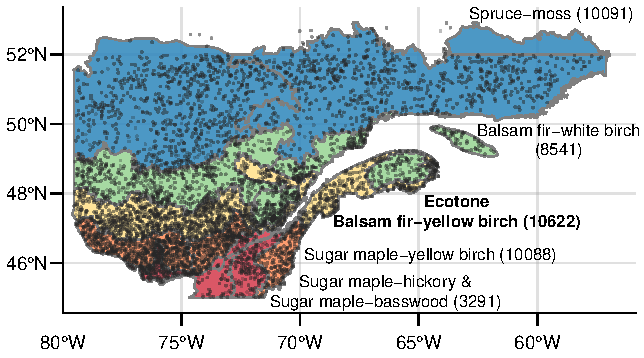
\includegraphics[width=5in,height=\textheight]{ms/figures/fig1_region.pdf}
\caption{Locations of the 6281 forest inventory plots in meridional
Québec, Canada. Colours delimit the six bioclimatic domains. The two
southernmost domains (orange) were combined in our analyses. The number
of forest plots in each domain is written in parentheses.}
\end{figure}

\hypertarget{environmental-variables}{%
\subsection{Environmental variables}\label{environmental-variables}}

The annual past climatic conditions, covering a period from 1960 to
2013, were extracted using a 2 km\textsuperscript{2} (60 arc sec)
resolution grid for the entire study area using the ANUSPLIN climate
modelling software (http://cfs.nrcan.gc.ca/projects/3/8; McKenney et
al., 2011). Bioclimatic variables hypothesised to influence tree
survival were intercepted at plot locations: the mean temperature and
total precipitation during the growing season, minimum temperature of
the coldest period, maximum temperature of the warmest period and the
annual climate moisture index (CMI; difference between annual
precipitation and potential evapotranspiration). From these bioclimatic
variables, we derived different predictors (see Table 1 for details).
Over the past four decades, growing season temperature and precipitation
have increased by 0.14 °C/decade and 9.5 mm/decade, respectively, while
CMI has decreased by 1.2 cm/decade (Fig. S1).

We also collected information pertaining to natural and anthropogenic
disturbances that have affected the forest plots both before and during
the study period (Table 1, Fig. S2). At each plot, 21 disturbance types
and their level of intensity (moderate or major) were recorded (Table
S2; MFFP, 2016). The MFFP defined major disturbances as events that
resulted in a loss of at least 75\% of the tree basal area, whereas
moderate disturbances have caused between 25\% and 75\% of loss. For our
regression models, we differentiated two main types of disturbances:
natural disturbances and harvest, with 3 levels of intensity each
(minor, moderate or major) and 2 periods (old: occurred before the first
inventory, and recent: occurred during the study period). To compare
diversity measures among disturbance levels, we also assigned each
forest to the level of intensity of the worst disturbance it experienced
(regardless of the type or timing).

Core samples were also collected on selected trees during surveys to
measure their age. Stand age was estimated as the mean of these measures
to account for forest succession processes after disturbances. Finally,
because the time interval between the first and last measurements varies
among the forest plots, it was included as a predictor.

\textbf{Table 1}. Description of the predictors used in the multiple
linear regression models. See Table S2 for details about disturbance
types.

\begin{longtable}[]{@{}ll@{}}
\toprule
\begin{minipage}[b]{0.22\columnwidth}\raggedright
Variable name\strut
\end{minipage} & \begin{minipage}[b]{0.72\columnwidth}\raggedright
Variable description\strut
\end{minipage}\tabularnewline
\midrule
\endhead
\begin{minipage}[t]{0.22\columnwidth}\raggedright
\textbf{Baseline conditions}\strut
\end{minipage} & \begin{minipage}[t]{0.72\columnwidth}\raggedright
\strut
\end{minipage}\tabularnewline
\begin{minipage}[t]{0.22\columnwidth}\raggedright
Temp, Temp\textsuperscript{2}\strut
\end{minipage} & \begin{minipage}[t]{0.72\columnwidth}\raggedright
Mean temperature during growing season and its second order polynomial.
10-year average prior to first survey of each plot (°C).\strut
\end{minipage}\tabularnewline
\begin{minipage}[t]{0.22\columnwidth}\raggedright
Precip, Precip\textsuperscript{2}\strut
\end{minipage} & \begin{minipage}[t]{0.72\columnwidth}\raggedright
Total precipitation during growing season and its second order
polynomial. 10-year average prior to first survey of each plot
(mm).\strut
\end{minipage}\tabularnewline
\begin{minipage}[t]{0.22\columnwidth}\raggedright
\(\Delta\)Time\strut
\end{minipage} & \begin{minipage}[t]{0.72\columnwidth}\raggedright
Time interval between first and last measurements (years).\strut
\end{minipage}\tabularnewline
\begin{minipage}[t]{0.22\columnwidth}\raggedright
\textbf{Climate change}\strut
\end{minipage} & \begin{minipage}[t]{0.72\columnwidth}\raggedright
\strut
\end{minipage}\tabularnewline
\begin{minipage}[t]{0.22\columnwidth}\raggedright
\(\Delta\)Temp\strut
\end{minipage} & \begin{minipage}[t]{0.72\columnwidth}\raggedright
Slope between Temp and time (°C/y).\strut
\end{minipage}\tabularnewline
\begin{minipage}[t]{0.22\columnwidth}\raggedright
\(\Delta\)Precip\strut
\end{minipage} & \begin{minipage}[t]{0.72\columnwidth}\raggedright
Slope between Precip and time (mm/y).\strut
\end{minipage}\tabularnewline
\begin{minipage}[t]{0.22\columnwidth}\raggedright
\(\Delta\)CMI\strut
\end{minipage} & \begin{minipage}[t]{0.72\columnwidth}\raggedright
Slope between Climate Moisture Index and time (cm/y)\}.\strut
\end{minipage}\tabularnewline
\begin{minipage}[t]{0.22\columnwidth}\raggedright
Temp min\strut
\end{minipage} & \begin{minipage}[t]{0.72\columnwidth}\raggedright
Extreme minimum temperature. Difference between minimum and mean
temperature of the coldest period (°C).\strut
\end{minipage}\tabularnewline
\begin{minipage}[t]{0.22\columnwidth}\raggedright
Temp max\strut
\end{minipage} & \begin{minipage}[t]{0.72\columnwidth}\raggedright
Extreme maximum temperature. Difference between maximum and mean
temperature of the warmest period (°C).\strut
\end{minipage}\tabularnewline
\begin{minipage}[t]{0.22\columnwidth}\raggedright
CMI min\strut
\end{minipage} & \begin{minipage}[t]{0.72\columnwidth}\raggedright
Extreme minimum Climate Moisture Index (CMI). Difference between minimum
CMI and mean CMI (cm), as a proxy of drought.\strut
\end{minipage}\tabularnewline
\begin{minipage}[t]{0.22\columnwidth}\raggedright
\textbf{Disturbances}\strut
\end{minipage} & \begin{minipage}[t]{0.72\columnwidth}\raggedright
\strut
\end{minipage}\tabularnewline
\begin{minipage}[t]{0.22\columnwidth}\raggedright
Age\strut
\end{minipage} & \begin{minipage}[t]{0.72\columnwidth}\raggedright
Stand age (years).\strut
\end{minipage}\tabularnewline
\begin{minipage}[t]{0.22\columnwidth}\raggedright
Old harvest\strut
\end{minipage} & \begin{minipage}[t]{0.72\columnwidth}\raggedright
Tree harvesting (clearcutting, partial cutting, selection cutting, etc.)
that occurred before the study period. 1. Minor (0), moderate (1) or
major (2).\strut
\end{minipage}\tabularnewline
\begin{minipage}[t]{0.22\columnwidth}\raggedright
Recent harvest\strut
\end{minipage} & \begin{minipage}[t]{0.72\columnwidth}\raggedright
Tree harvesting (clearcutting, partial cutting, selection cutting, etc.)
that occurred during the study period. Minor (0), moderate (1) or major
(2).\strut
\end{minipage}\tabularnewline
\begin{minipage}[t]{0.22\columnwidth}\raggedright
Old natural\strut
\end{minipage} & \begin{minipage}[t]{0.72\columnwidth}\raggedright
Natural disturbances (fire, insect outbreak, windfall, etc.) that
occurred before the study period. Minor (0), moderate (1) or major
(2).\strut
\end{minipage}\tabularnewline
\begin{minipage}[t]{0.22\columnwidth}\raggedright
Recent natural\strut
\end{minipage} & \begin{minipage}[t]{0.72\columnwidth}\raggedright
Natural disturbances (fire, insect outbreak, windfall, etc.) that
occurred before the study period. Minor (0), moderate (1) or major
(2).\strut
\end{minipage}\tabularnewline
\bottomrule
\end{longtable}

\hypertarget{analysis}{%
\subsection{Analysis}\label{analysis}}

\hypertarget{uxdf-diversity}{%
\subsubsection{ß diversity}\label{uxdf-diversity}}

For each plot, we computed temporal ß diversity (Legendre, 2019), which
is the dissimilarity in species composition between two surveys of a
given plot, by comparing local tree abundance (i.e.~number of
individuals) in forest plots between the historical (1970-1980, \(t_1\))
and contemporary (2000-2016, \(t_2\)) periods. The dissimilarity (ß) was
computed using the Ružička coefficient (Fig. S3):

\(\beta = (B+C)/(A+B+C)\) where, for \(n\) species:

\(A = \sum_{j=1}^n a_j\)~: unscaled similarity. \(a_j\) represents the
abundance of species \(j\) that is common between \(t_1\) and \(t_2\);~

\(B = \sum_{j=1}^n b_j\)~: unscaled species abundance losses. \(b_j\)
represents the abundance of species \(j\) present at \(t_1\) but not at
\(t_2\); when species \(j\) increases in abundance, \(b_j\) = 0;

\(C = \sum_{j=1}^n c_j\)~: unscaled species abundance gains. \(c_j\)
represents the abundance of species \(j\) present at \(t_2\) but not at
\(t_1\); when species \(j\) decreases in abundance, \(c_j\) = 0;

This temporal ß diversity varies from 0 (community compositions at
\(t_1\) and \(t_2\) are exactly the same) to 1 (communities have no
shared species). The use of this dissimilarity index enabled us to
decompose the compositional change into relative gains (\(C/(A+B+C)\))
and losses (\(B/(A+B+C)\)) in tree abundances (Fig. S3). Throughout this
paper, gains and losses refer to these relative metrics.

This additive framework allowed us to partition further the different
components contributing to ß diversity. Temporal dissimilarity in tree
community can be decomposed into the dissimilarity (gains and losses) of
different species groups of interest, here boreal, pioneer and temperate
species (Table S1). The temporal dissimilarity of a given group, for
instance boreal, relative to all species is simply:
\(\beta_{boreal} = (B_{boreal}+C_{boreal})/(A+B+C)\), with \((A+B+C)\)
the denominator computed over all tree species. As a consequence, ß can
be decomposed as follows:

\(\beta = \beta_{boreal} + \beta_{pioneer} + \beta_{temperate}\)

\hypertarget{assessing-the-relative-importance-of-drivers-of-community-changes}{%
\subsubsection{Assessing the relative importance of drivers of community
changes}\label{assessing-the-relative-importance-of-drivers-of-community-changes}}

We evaluated the effects of multiple drivers on temporal ß, gains and
losses using multiple regressions, in combination with variation
partitioning analyses (Borcard et al., 1992; Peres-Neto et al., 2006).
For these analyses, we used a logit transformation \(y'=log(y/(1-y))\)
of the response variables (ß, gains, losses) as they were all in the
standard unit range {[}0, 1{]}.

In order to quantify the variation explained by climate change and
disturbances, while controlling for the baseline climate gradient and
different time intervals, we classified our predictor variables into
three subsets: baseline conditions, climate change and disturbances (see
Table 1). We then generated regression models predicting ß, gains and
losses, for each of the three subsets. We also tested relevant
interactions between disturbance and climate predictors: Natural (old
and recent) \(\times\) \(\Delta\)CMI and Natural (old and recent)
\(\times\) \(\Delta\)Temp, because drought and heat stress can increase
natural disturbance frequency; Harvest (old and recent) \(\times\)
\(\Delta\)Temp), because the effect of harvest was hypothesised to be
influenced by warmer temperatures. A forward selection of explanatory
variables based on two stopping criteria (significance level \(\alpha\)
and global \(R^2_{adj}\); Blanchet et al., 2008) was performed to obtain
parsimonious regression models for each of the three subsets. The
predictors had been previously standardised to \emph{z}-scores to allow
comparison of their slope coefficients. We also ensured that residuals
met the assumptions of normality and homoscedasticity.

We assessed the unique contributions of each predictor subset (baseline
conditions, climate change and disturbances) as well as their shared
effect on forest community changes using variation partitioning analysis
on the parsimonious regression models.

\hypertarget{functional-index-of-community-change}{%
\subsubsection{Functional index of community
change}\label{functional-index-of-community-change}}

To test whether or not climate warming contributed to community changes,
we examined the temporal changes in the distribution of species
temperature values within every plot. We quantified such changes by the
shift in the mean (Community Temperature Index or CTI; Devictor et al.,
2008), as well as the lower 10\textsuperscript{th} percentile and the
upper 90th percentile of this plot-level distribution (De Frenne et al.,
2013).

To compute these metrics, we first combined climate and tree occurrence
data to obtain species temperature distributions. Specifically, we
overlaid interpolated climate data (mean annual temperature averages for
1970--2000 at a spatial resolution of 1 km\textsuperscript{2}, available
online http://worldclim.org/version2; Fick \& Hijmans, 2017) and
occurrence data from multiple forest inventory databases of eastern
North America (collected in the QUICC-FOR project;
https://github.com/QUICC-FOR) for the focal species. The mean annual
temperature for each occurrence was extracted to infer species
temperature distributions. Following Devictor et al. (2008), we used the
mean of these temperature values as a proxy for species thermal
preference (Species Temperature Index, STI, in Celsius; Table S1). For
each plot in each time period, the CTI was then calculated as the mean
of the STI values weighted by the abundances of the species present in
that plot.

Following De Frenne et al. (2013), we computed the
10\textsuperscript{th} and 90\textsuperscript{th} percentiles of the
plot-level temperature distributions, which correspond to the cold and
warm tails of the distribution. To do so, for every plot and every
species, we sampled 1000 temperature values per individual from the
species' temperature distribution. The plot-level temperature
distributions corresponds to the combination of the temperature values
for all individuals in a given plot. From these distributions, which
accounted for species composition and their relative abundances, we
computed the 10\textsuperscript{th} and 90\textsuperscript{th}
percentiles. Note that contrary to De Frenne et al. (2013), we used the
entire distribution for each species instead of modelling species
thermal response curves because numerous species distributions were not
Gaussian.

To evaluate the directionality of the changes in communities between the
historical (\(t_1\)) and contemporary (\(t_2\)) periods, we computed the
temporal shift in the mean CTI, the cold tail and the warm tail (in °C
per decade) as follows:

\(\Delta CTI = \frac{CTI_{t2} - CTI_{t1}}{t_2 - t_1} \times 10\)

The shifts in the cold and warm tails were computed in the same way as
for the shifts in mean CTI. A positive value of \(\Delta\)CTI indicates
an overall thermophilization of the tree community in degrees per
decade. A positive shift of the cold tail indicates a decrease of
cold-adapted species, while a positive shift of the warm tail indicates
an increase of warm-adapted species; both result in thermophilization.

We also quantified how each species contributed to \(\Delta\)CTI through
gain or loss in abundances. Species contributions were assessed
following these steps: for each species, (1) we replaced its abundance
at \(t_2\) by its abundance at \(t_1\), as if this species abundance had
not changed over time; (2) we computed a new CTI\textsubscript{t2}`; (3)
then we calculated \(\Delta\)CTI' using CTI\textsubscript{t2}' and
CTI\textsubscript{t1} as above; and (4) we measured the difference
between \(\Delta\)CTI' and \(\Delta\)CTI in each plot. A positive value
indicates that the change (gain or loss) of a given species abundance
increases thermophilization in a plot. Then, we determined the role of
species gains and losses in \(\Delta\)CTI by averaging their
contributions for plots where they increased and where they decreased.

To test the hypothesis that community changes are resulting from
post-disturbance succession, we collected traits about species shade
tolerance (Species Shade Index, SSI; Niinemets \& Valladares, 2006),
which represents a species ability to grow in shade conditions. Shade
tolerance indices ranged from 1 (very intolerant to shade) to 5 (very
tolerant) on a continuous scale. As for CTI, a Community Shade Index
(CSI) was computed for each plot as the mean of the SSI values weighted
by the abundances of the species present in that plot. Temporal shift in
CSI between the historical and contemporary time periods, \(\Delta\)CSI,
was computed in the same way as for \(\Delta\)CTI, where a positive
value indicates a progress in stand succession toward climax, in units
per decade.

All analyses were performed using the R programming language version
3.5.1 (R Core Team, 2018). The list of R packages that have been used
throughout the analysis is provided in Table S3. All the data used in
the study as well as R scripts to reproduce the analyses and the figures
can be found online at https://github.com/mhBrice/thermophilization
(https://doi.org/10.5281/zenodo.3242773).

\hypertarget{results}{%
\section{Results}\label{results}}

\hypertarget{temporal-uxdf-diversity}{%
\subsection{Temporal ß diversity}\label{temporal-uxdf-diversity}}

The mean temporal ß diversity was 0.56 over all sites in the study area
(\emph{n} = 6281), and these temporal changes in composition were
attributable to slightly more gains in abundances (52.5\%) than losses
(47.5\%; Fig. 2a). Temporal ß diversity varied along a latitudinal
gradient; it tended to decrease northward, reaching its maximum at 48°N
of latitude, which corresponds to the northern limit of the balsam
fir-yellow birch domain, the ecotone between boreal and deciduous
forests. North of the 49°N of latitude, in the spruce-moss domain,
temporal ß changes were dominated by losses whereas, south of this
limit, gains prevailed. Latitudinal patterns were also visible in the
contributions of the three species groups to temporal ß (Fig. 2b). At
minor disturbance level, community changes were mainly determined by
gains in temperate species south of 47°N and by gains in boreal species
north of 47°N (where boreal species are the most abundant species
group).

\begin{figure}
\centering
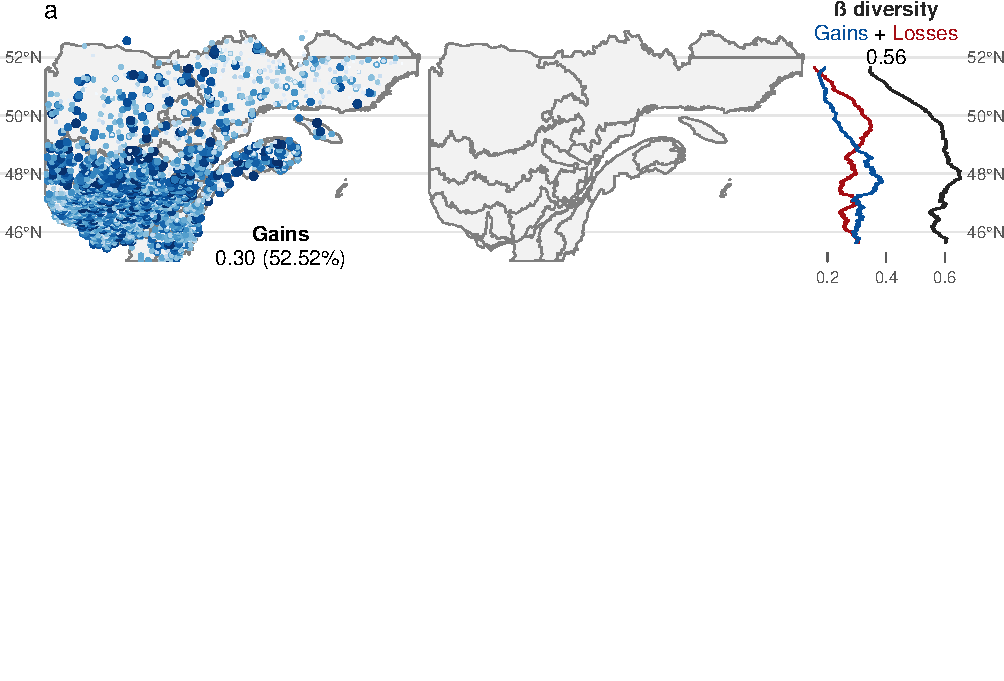
\includegraphics[width=6.7in,height=\textheight]{ms/figures/fig2_map_roll.pdf}
\caption{Maps of gains and losses in tree abundances (a) and latitudinal
trends in temporal ß diversity, decomposed into gains (blue) and losses
(red) of boreal, pioneer and temperate trees, for different levels of
disturbance (b-d). The sizes and colours of the points on the maps are
proportional to the values of interest. The latitudinal trends in
temporal ß in a-d are based on moving averages computed on each index
against latitude (window size of 500 plots in panel a and 400 plots in
panels b-d), to smooth out local-scale fluctuations and highlight
broad-scale trends.}
\end{figure}

The magnitude of compositional changes in forests was highly influenced
by disturbances (Figs 2b-d, 3, S4). In each domain, the ß diversity
values of highly disturbed forests are strongly skewed (Fig. 3). The
mean temporal ß was 0.43 at minor disturbance level, whereas it was 0.53
at moderate disturbance level and reached 0.74 at major disturbance
level (all domains combined). Moreover, the fraction of changes
attributed to losses was generally lower at minor, than at moderate and
major disturbance levels (minor: 41\%; moderate: 48\%; major: 50\%, all
domains combined), especially for the spruce-moss domain (minor: 40\%;
moderate: 73\%; major: 64\%; Fig. 3). At minor disturbance level, both
boreal and temperate species groups experienced more gains than losses
(Fig. 2b), while at major disturbance level, we observed a strong surge
in losses of boreal tree species along with larger gains of pioneer
species (Fig. 2d). In contrast, gains in temperate species were higher
at moderate disturbance level (Fig. 2c). Some species have experienced
great changes in abundance and occurrence throughout these domains,
namely \emph{Picea mariana}, \emph{Acer rubrum}, \emph{Betula
alleghaniensis}, \emph{Fagus grandifolia} and \emph{Populus
tremuloides}, and likely contributed largely to the pattern of temporal
ß diversity (Fig. S5).

\begin{figure}
\centering
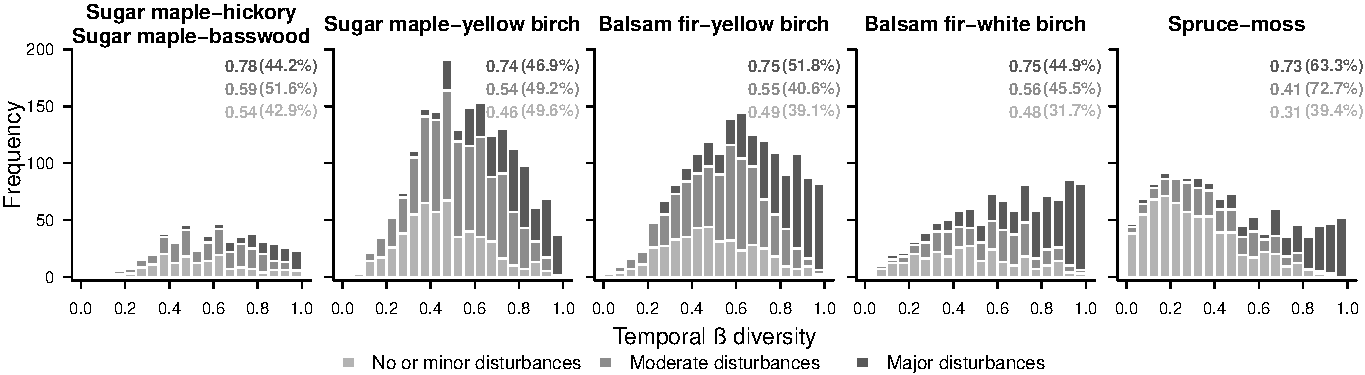
\includegraphics[width=6.7in,height=\textheight]{ms/figures/fig3_hist.pdf}
\caption{Frequency distributions of temporal ß diversity in forests
plots by bioclimatic domains. Forests of different disturbance levels
are stacked on top of each other. The values written in the panels are
the mean temporal ß diversity values followed by the percentage of
losses in parentheses. The distribution of ß diversity values is skewed
to the right for higher disturbance levels.}
\end{figure}

\hypertarget{drivers-of-temporal-changes}{%
\subsection{Drivers of temporal
changes}\label{drivers-of-temporal-changes}}

Once combined, predictors from the three subsets (baseline, climate
change and disturbances; Table 1) explained together 40\% of the
variation of temporal ß diversity, and 30\% for both gains and losses
(Fig. 4). As revealed by the variation partitioning analyses, community
temporal changes were mainly driven by disturbances (\(R^2_{adj}\) for
ß: 31\%; gains: 25\%; losses: 26\%), whereas the unique influence of
climate change as well as that of baseline conditions were significant
but comparatively modest (\(R^2_{adj}\) \textless{} 1\%; Fig. 4d-f).

Overall, disturbances enhanced temporal ß diversity, with old major
harvest (Old harvest\textsubscript{2}) being the most important driver,
followed by old major natural disturbances (Old
natural\textsubscript{2}; Fig. 4a-c). Interestingly, while recent
disturbances (natural and harvest) promoted losses and reduced gains,
old disturbances had the opposite effect (Fig. 4b-c). As
time-since-disturbance increased and the forests grew old (Age), forest
composition changed less and colonisation by new individuals became less
frequent (Fig. 4a-b).

Regression models provided only weak evidence of climate change effect
on forest community changes. Mainly, extreme minimum climate moisture
index (CMI min) and extreme cold (Temp min) contributed to community
changes through losses in tree abundances (Fig. 4a,c). Increase in
precipitation (\(\Delta\)Precip) favoured tree gains. Only one
interaction was retained, which indicated that stronger warming
(\(\Delta\)Temp) mitigated the effect of recent moderate harvest (Recent
harvest\textsubscript{1}) on losses. Variables related to baseline
conditions were more important than climate change variables; the
effects of mean temperature (Temp) and total precipitation (Precip)
likely reflect the latitudinal gradient in community change, while the
effect of time interval between surveys (\(\Delta\)Time) reflects the
fact that community change takes time.

\begin{figure}
\centering
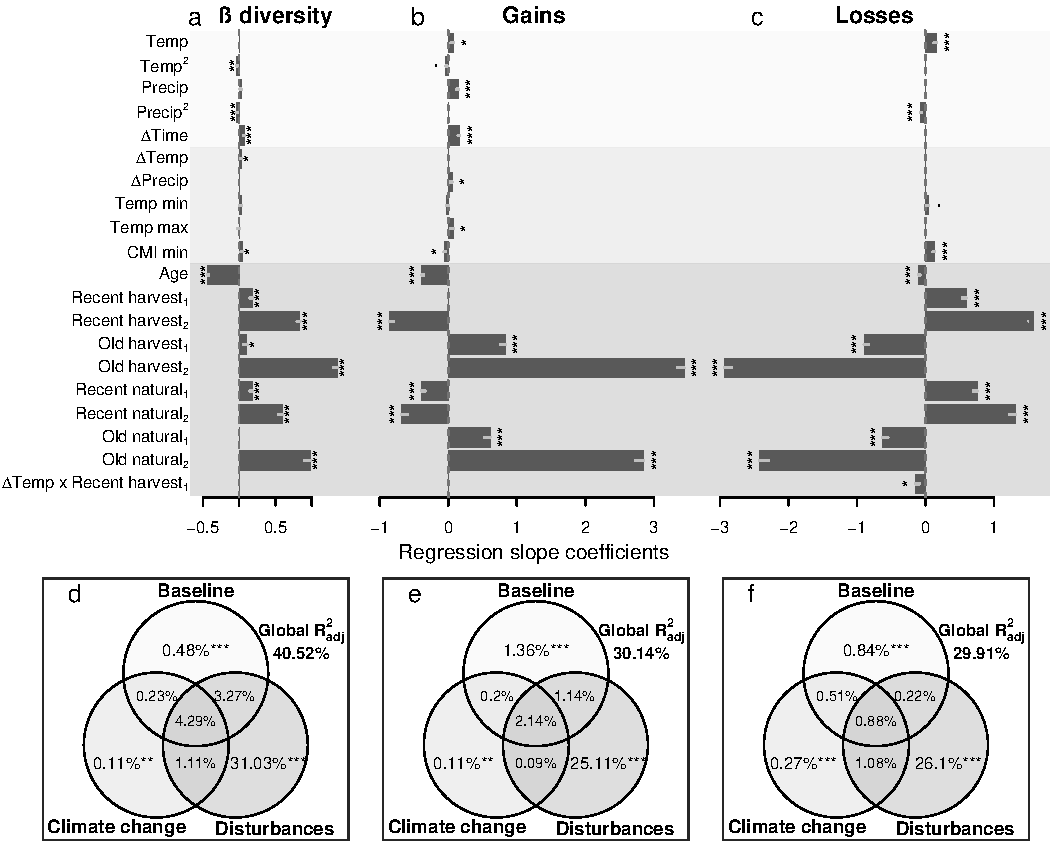
\includegraphics[width=6.6in,height=\textheight]{ms/figures/fig4_reg.pdf}
\caption{Slope coefficients from multiple regression models for (a)
temporal ß diversity, (b) species gains and (c) species losses and the
corresponding variation partitioning diagrams (d, e, f). Error bars
represent one standard error of the slope coefficient. For the
regression models, only the selected predictors are shown. Subscripts
following disturbance predictors indicate their levels of intensity: 1
Moderate and 2 Major. In each variation partitioning, significance of
each unique fraction was tested using 9999 permutations, while shared
fractions cannot be tested. Stars indicate the level of significance of
the \emph{p}-values (* \emph{p} \textless{} 0.05; ** \emph{p}
\textless{} 0.01; *** \emph{p} \textless{} 0.001). See Table 1 for
description of the predictor variables.}
\end{figure}

\hypertarget{changes-in-community-temperature-and-shade-indices}{%
\subsection{Changes in community temperature and shade
indices}\label{changes-in-community-temperature-and-shade-indices}}

The community temperature index (CTI) increased significantly between
the historical and contemporary periods (paired \emph{t}-test
\emph{p}-value \textless{} 0.001; mean of +0.03 °C/decade for all plots
combined, ranging from -0.02 to +0.05 across domains), which indicates a
generalised community thermophilization throughout the study area.
During the same time period, the community shade index (CSI) also
increased (+0.01 unit/decade), suggesting a transition towards late
successional forests (Fig. 5).

Thermophilization was significantly larger in moderately disturbed
forests (\(\Delta\)CTI = +0.044 °C/decade) than in undisturbed (+0.015
°C/decade) or highly disturbed forests (+0.018 °C/decade; ANOVA
\(F_{2, 6278}\) = 14.59, \emph{p}-value \textless{} 0.001; a post-hoc
Tukey test showed significantly higher \(\Delta\)CTI at moderate
disturbance than at the other levels). Moreover, the latitudinal pattern
of \(\Delta\)CTI varied with the disturbance level: the
thermophilization in moderately disturbed forests extended further north
than in undisturbed forests, exceeding 48°N, up in the balsam fir-yellow
birch domain (Fig. 5b,e), while at major disturbances, thermophilization
was more or less constant across the latitudinal gradient (Fig. 5c,f).
Despite the influence of disturbances on thermophilization, change in
CTI was weakly explained by our complete set of environmental predictors
(\(R^2_{adj}\) ca. 3\%). Moreover, the relationship between
thermophilization and climate change predictors was surprisingly weak
(\(R^2_{adj}\) \textless{} 1\%), with no correlation at all with
temperature change.

The analysis of \(\Delta\)CSI revealed that major disturbances resulted
in a large decrease in CSI (Fig. 5c; mean \(\Delta\)CSI = -0.037),
consistent with higher gains in pioneer species (Fig. 2), while minor
disturbances led to an increase in CSI (Fig. 5a; mean \(\Delta\)CSI =
+0.060). Both influenced by disturbances, \(\Delta\)CTI and
\(\Delta\)CSI were negatively correlated (Pearson \emph{r} = -0.2,
\emph{p}-value \textless{} 0.001) indicating that the two ecological
processes are intertwined. However, \(\Delta\)CTI was more strongly
correlated to gains in temperate species and losses of boreal species
than to gains in pioneer species (Fig. S6), which suggests that
thermophilization was not trivially driven by successional processes.

Community thermophilization was asymmetrical and mainly driven by larger
gains in warm-adapted species, as indicated by the larger increases in
the warm-tail of the temperature distributions than in the cold-tail
(Fig. 5d-f). Moderate disturbances exacerbated this effect from the
sugar maple-yellow birch up to the balsam fir-white birch domain (larger
increase in the warm tail; Fig. 5e). The positive correlation between
\(\Delta\)CTI and gains in temperate species in all domains, except in
the spruce-moss, also corroborates the role of warm-adapted species
(Fig. S6).

\begin{figure}
\centering
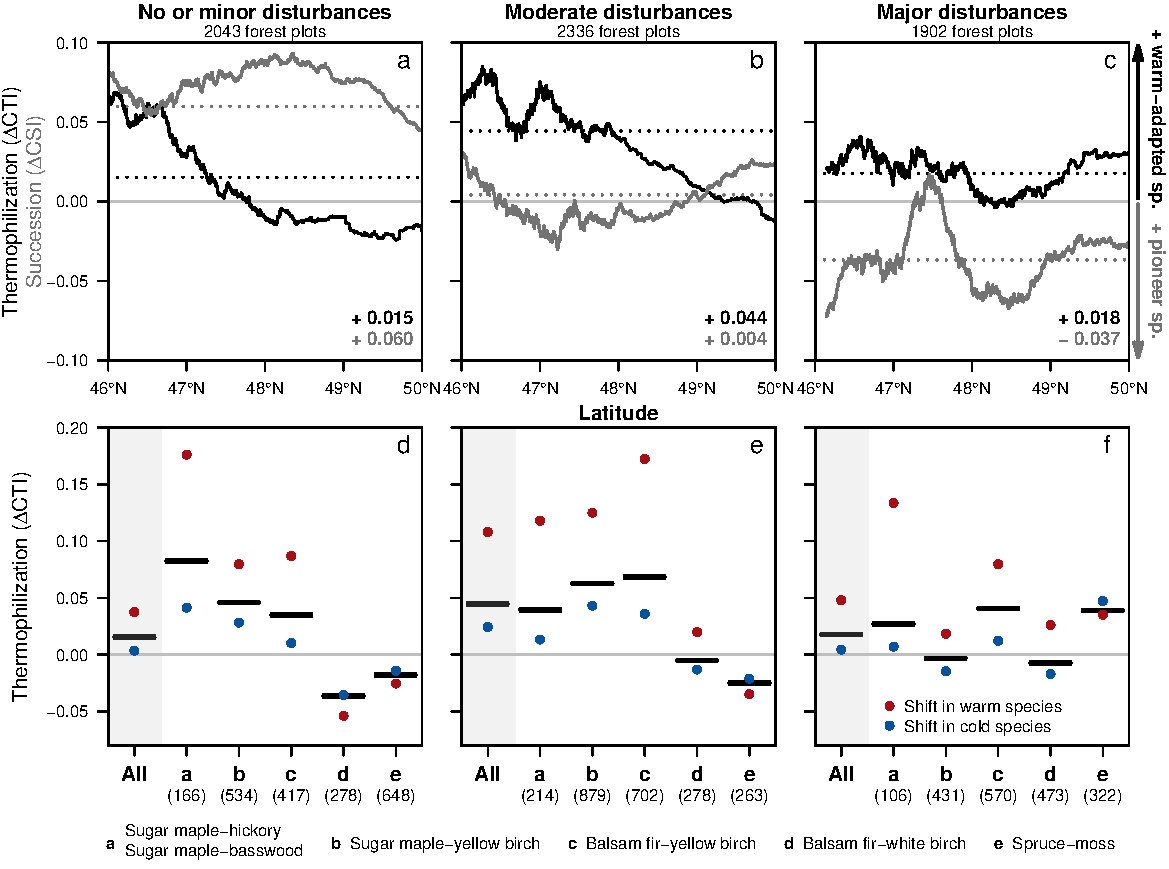
\includegraphics[width=6.6in,height=\textheight]{ms/figures/fig5_thermo.pdf}
\caption{Thermophilization (i.e., change in community temperature index,
\(\Delta\)CTI) and successional process (i.e., change in community shade
index, \(\Delta\)CSI) of forests for different levels of disturbance. In
the upper panels (a-c), the latitudinal trends in \(\Delta\)CTI (black
curve) and \(\Delta\)CSI (grey curve) are based on moving averages
computed on the indices against latitude (window size of 400 plots).
Positive values indicate an increase in warm-adapted species (black) or
in late-successional species (grey) over time. The dotted lines in
panels a-c represent the mean \(\Delta\)CTI (black) and \(\Delta\)CSI
(grey) values for different levels of disturbance. The lower panels
(d-f) show thermophilization of the forest plots across the study area
(All) and by bioclimatic domain. Positive values for the temporal shift
of the mean (black line), left tail (red) and right tail (blue) of the
distribution of CTI indicate overall thermophilization, increases of
warm‐adapted and decreases of cold‐adapted species, respectively.}
\end{figure}

Only a few species contributed substantially to community
thermophilization (Fig. 6). Gains of \emph{Acer rubrum} and \emph{Acer
saccharum}, as well as losses of \emph{Abies balsamea} and \emph{Picea
mariana}, contributed strongly to the thermophilization of all
bioclimatic domains. In addition to the change of these four species,
the losses of \emph{Betula papyrifera} and \emph{Picea glauca} also
played a key role in the thermophilization of ecotonal forests in the
balsam fir-yellow birch domain. Moreover, temperate species such as
\emph{Fagus grandifolia}, \emph{Quercus rubra} and \emph{Fraxinus
americana} contributed mostly to the thermophilization of southern
domains (Fig. 6) where their abundance has increased (Fig. S5). In
contrast, the surge in CTI north of the 49°N (spruce-moss) in highly
disturbed forests (Fig. 5) was likely due to the replacement of boreal
species by pioneer species (Fig. S6), such as \emph{Betula papyrifera}
and \emph{Salix spp.} (Fig. 6).

\begin{figure}
\centering
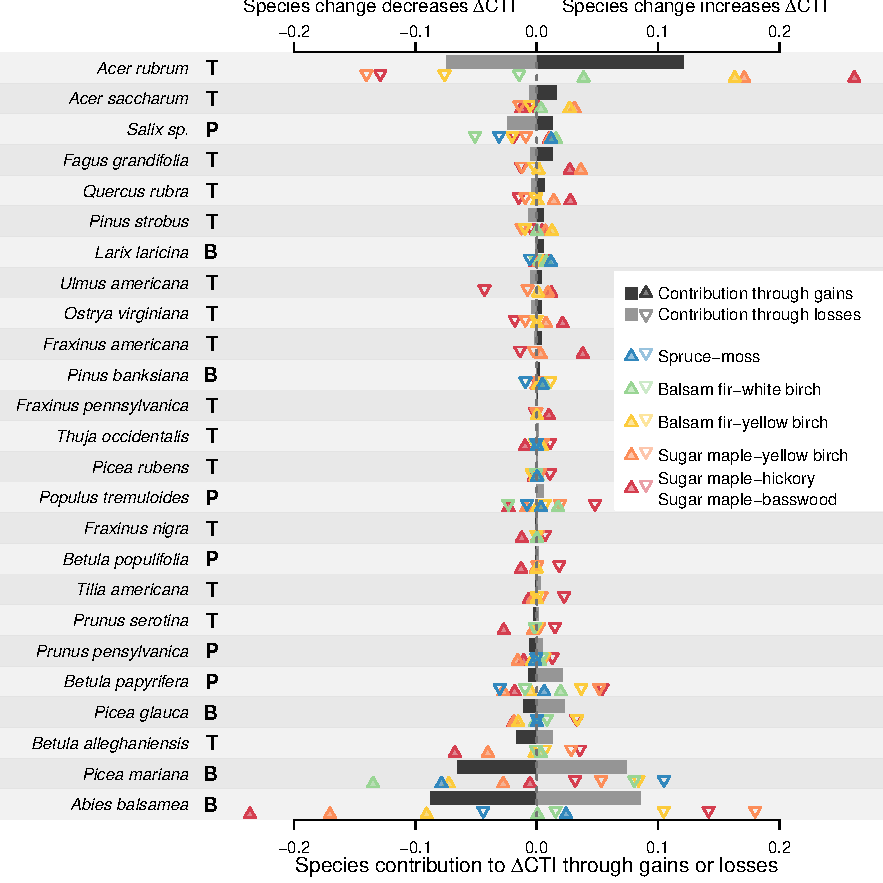
\includegraphics[width=5.8in,height=\textheight]{ms/figures/fig6_spcontrib_cti.pdf}
\caption{Individual species contributions, through gains and losses, to
thermophilization of forest communities across the study area and for
each bioclimatic domain. The bars represent the mean contributions of
given species through gains (dark grey) or losses (light grey) across
the study area, while the coloured triangles represent the mean
contributions of given species through gains (filled) or losses (open)
by domain. For example, the \(\Delta\)CTI increased by an average of
0.12 for all plots where \emph{Acer rubrum} has increased in abundance
(dark grey bar), whereas the \(\Delta\)CTI also increased by an average
of 0.09 for all plots where \emph{Abies balsamea} has decreased in
abundance (light grey bar). Letters next to species names correspond to
(T)emperate, (P)ioneer and (B)oreal species. Only species that
contributed more than 0.01 in at least one domain are shown.}
\end{figure}

\hypertarget{discussion}{%
\section{Discussion}\label{discussion}}

Taken together, our results suggest that disturbances accelerate tree
community responses to climate change, revealing potential synergies
that are yet to be investigated. Local and short-term influences of
disturbances mask long-term and lagging climate-induced changes in
communities. Yet, we revealed a generalised thermophilization of forests
throughout the temperate-boreal ecotone of Québec, driven by a
concurrent gain of temperate species and loss of boreal species.
Moreover, we found that moderate disturbances likely accelerated
thermophilization. Hence, moderate disturbances, but not major ones,
could facilitate gains in warm-adapted species under climate change.

\hypertarget{impact-of-disturbances-on-tree-community-changes}{%
\subsection{Impact of disturbances on tree community
changes}\label{impact-of-disturbances-on-tree-community-changes}}

Our results suggest that disturbances (e.g., clear-cutting, insect
outbreaks, fires) are the primary drivers of forest community changes in
the temperate-boreal ecotone. Such findings are in agreement with
previous work showing that disturbances alter rapidly and profoundly
tree communities that otherwise respond slowly to environmental changes
(Vanderwel et al., 2013).

Furthermore, our study underscores the importance of historical
disturbances, particularly harvesting activities, on the forest dynamics
of the temperate-boreal ecotone. Disturbance effects on communities may
persist from decades to centuries (Johnstone et al., 2016) and, here,
the effects of historical disturbances even superseded that of recent
disturbances. Such findings stress that disturbances cannot be ignored
when modelling the future of forests with climate change, as they not
only drive community changes, but also have long-lasting impacts. Tree
harvesting was the most frequent type of disturbance (Fig. S2) and alone
accounted for 24.7\% of all tree mortality during the study period, thus
impacting severely all components of temporal community changes.
However, in contrast to natural disturbances, tree harvesting has been
shown to disrupt the relationship between vegetation and local
environmental conditions and, because of its short return interval, to
favour young even-aged stands to the detriment of old-growth forests
(Boucher et al., 2009; Boucher \& Grondin, 2012).

\hypertarget{climate-induced-change-in-tree-community}{%
\subsection{Climate-induced change in tree
community}\label{climate-induced-change-in-tree-community}}

Our findings highlight an ongoing shift toward more warm-adapted tree
species in forests across the temperate-boreal ecotone. This overall
thermophilization trend of tree communities is consistent with the
hypothesis of climate-induced range shift, expanding on earlier findings
that forests are responding to climate warming (e.g.~Sittaro et al.,
2017; Fisichelli et al., 2014; Leithead et al., 2010). However, the
observed increase of tree community temperature of +0.03 °C/decade is
considerably smaller than the rising trend in growing season temperature
of 0.14 °C/decade (Fig. S1). Although these measures have different
origins and should thus be compared cautiously, our findings support the
conclusion of numerous studies that tree responses often lag behind
environmental changes (Renwick \& Rocca, 2015; Sittaro et al., 2017;
Svenning \& Sandel, 2013; Talluto et al., 2017). Considering the
velocity of the predicted future climate change, the gap between species
distributions and their optimal climate niches will likely widen and
lead to greater reshuffling of biodiversity.

\hypertarget{feedback-between-climate-change-and-disturbances}{%
\subsection{Feedback between climate change and
disturbances}\label{feedback-between-climate-change-and-disturbances}}

Our most striking finding is that community thermophilization was
amplified by moderate disturbances. Our combined analysis of change in
CTI and CSI also allowed us to disentangle climate change effects from
successional processes, highlighting that the observed thermophilization
was not simply correlated with the replacement of boreal by pioneer
species. Our work provides a broad-scale community perspective on the
role played by disturbances in promoting northward migration of tree
species, which is in agreement with the conclusions of recent empirical
(Boucher et al., 2006; Leithead et al., 2010) and simulation (Vanderwel
\& Purves, 2014; Wang et al., 2015) studies.

Disturbances likely accelerate forest changes by reducing competition
and providing establishment opportunities to warm-adapted temperate tree
species (Leithead et al., 2010; Svenning \& Sandel, 2013). Indeed, in
the absence of disturbances, trees grow slowly, their mortality rates
are low and competition for space and light is strong, thus preventing
warm-adapted species from colonizing new areas, despite the suitability
of climatic conditions; community thermophilization is consequently very
slow. Moderate disturbances, however, remove individuals of resident
species and reduce competition, which enhances the replacement of boreal
by temperate trees, thereby increasing the thermophilization rate.
Furthermore, moderate disturbances can also modify local microclimates
(De Frenne et al., 2013; Stevens et al., 2015) which may alter the
survival rates of tree saplings. In contrast, major disturbances only
favour early successional species. Such findings echo the well-known
intermediate disturbance hypothesis (Connell, 1978); as in the classical
hypothesis, intermediate disturbances lower interspecific competition
but here, not only do they increase local species richness (not shown),
but they also accelerate ecological transitions.

Our complete set of predictors poorly explained the observed forest
thermophilization, likely because this process was highly variable among
localities. Forest composition is thus changing as expected under
climate warming, but thermophilization does not appear to be directly
driven by rising temperatures. As suggested by Renwick \& Rocca (2015),
we surmise that, as climate warms up, moderate disturbances could foster
punctuated and episodic migration of warm-adapted species in localities
where conditions are otherwise favourable. However, it raises questions
about the specific conditions in which the thermophilization process can
effectively take place. Further analyses are required to determine which
factors can trigger (e.g.~type, size, frequency of disturbances) or
constrain (e.g.~soil type, competition, precipitation) the invasion by
warm-adapted species.

Our results contrast with those of Boisvert‐Marsh et al. (2019) who
found that climate was more important than disturbances in explaining
tree sapling recruitment at their northern limit in Québec. This
suggests that the pattern we uncovered might be primarily caused by an
increase in abundance of species already present rather than by new
colonization. Danneyrolles et al. (2019) also found that forest
compositional changes over the last centuries (between 1790--1900 and
1980--2010) in deciduous forests of southern Québec were largely driven
by land-use changes, favouring more disturbance-adapted tree species,
but did not find any signs of thermophilization. In contrast to our
study that covers a period of pronounced climate warming, Danneyrolles
et al. (2019) investigated a period dominated by land-use and population
changes which may explain the absence of thermophilization signal in
their results. In light of their results, we hypothesise that some of
the thermophilization we reported here in the sugar maple domains is in
fact the result of secondary succession after historical disturbances.

\hypertarget{species-contributions-to-community-thermophilization}{%
\subsection{Species contributions to community
thermophilization}\label{species-contributions-to-community-thermophilization}}

We found that the observed community thermophilization was caused by
gains and losses in abundance of a restricted group of species. This
differential rate of species response entails that other species lag
even more behind climate change and that larger reshuffling of
communities is still ahead of us. The interaction between climate and
disturbances likely promotes generalist tree species adapted to
disturbances with high dispersal abilities (Aubin et al., 2016). For
instance, generalist species like \emph{Acer sp.}, especially \emph{Acer
rubrum}, have been expanding in eastern North America since the
pre-industrial period (Boucher et al., 2006; Danneyrolles et al., 2019;
Thompson et al., 2013) and recently established themselves in boreal
forests (Leithead et al., 2010; Sittaro et al., 2017) because they
quickly take advantage from disturbances and thrive in a wide variety of
ecological conditions. In contrast, some species limited by dispersal,
such as \emph{Carya sp.} and \emph{Tilia americana}, or constrained to
specific habitat, such as \emph{Acer saccharinum}, might not benefit
from these opportunities.

The magnitude of change in CTI varied by bioclimatic domains reflecting
the spatial patterns of species changes in response to climate warming
and disturbances. The thermophilization of the sugar maple domains was
facilitated by the presence of a large pool of warm-adapted species.
When disturbed, these southernmost domains had lower thermophilization
because they gained pioneer species. We showed that the balsam
fir-yellow birch domain was particularly sensitive to moderate
disturbances. The thermophilization of this ecotonal zone was primarily
due to increase in \emph{Acer rubrum} and, to a lesser extent, increase
in \emph{A. saccharum} and decrease in \emph{Abies balsamea} and
\emph{Betula papyrifera}. Although \emph{A. rubrum} is already well
established in this domain, our results suggest that it will continue to
thrive and spread, likely in response to a combination of climate
warming, historical and recent disturbances as well as natural forest
dynamics. \emph{A. saccharum} is presently constrained on hilltops in
the southern part of this domain (Gosselin, 2002), but our results
suggest that it could expand in nearby habitats. In contrast, the
decrease in CTI in the balsam fir-white birch and spruce moss domains
could be explained by the fact that temperate species are rare in these
two northernmost domains, hence changes in CTI resulted mostly from a
dynamic of replacement between pioneer and boreal species in response to
disturbances. \emph{A. rubrum} was the only temperate species to
increase in the balsam fir-white birch domain (Fig. S5) and, when it
did, it contributed to increase its CTI (Fig. 6). Similarly to \emph{A.
saccharum}, \emph{A. rubrum} distribution is spatially constrained
within the balsam fir-white birch domain (Blouin \& Berger, 2008) and
will likely expand from existing existing patchy populations in the
future.

\hypertarget{long-term-perspectives-for-the-temperate-boreal-ecotone}{%
\subsection{Long-term perspectives for the temperate-boreal
ecotone}\label{long-term-perspectives-for-the-temperate-boreal-ecotone}}

Although the time period covered by our study (46 years) is sufficient
to observe significant trends in forest compositional changes, it is not
long enough to test whether warm-adapted temperate species will persist
and thrive in these novel assemblages or if boreal species will
out-compete them in the long run. Therefore, an important question
remains: does the current forest thermophilization indicates an ongoing
ecosystem shift or only a transient dynamic? Multiple studies suggest a
persistence of these novel assemblages. For instance, after a century of
logging disturbances, temperate species were found to have increased and
persisted in forests formerly dominated by conifers (Boucher et al.,
2006). Furthermore, Fréchette \& de Vernal (2013) provided evidence
that, during the last interglacial period (6-7°C warmer), the northern
limit of the temperate biome was located about 500 km north of its
actual limit, suggesting that a northward shift of the ecotone is
possible. Hence, while climate warming erodes forest resilience by
affecting competitive advantages and generating colonization debt, our
findings suggest that moderate disturbances play a major role in
promoting regime shift by speeding up the transition from one ecosystem
state to another. Such a conclusion stresses the importance of
accounting for the synergistic effect of disturbances and climate change
in forest management strategies as well as in models of forest responses
to climate change.

\pagebreak

\hypertarget{references}{%
\section{References}\label{references}}

\hypertarget{refs}{}
\leavevmode\hypertarget{ref-allen_global_2010}{}%
Allen, C. D., Macalady, A. K., Chenchouni, H., Bachelet, D., McDowell,
N., Vennetier, M., Kitzberger, T., Rigling, A., Breshears, D. D., Hogg,
E. H. (., Gonzalez, P., Fensham, R., Zhang, Z., Castro, J., Demidova,
N., Lim, J.-H., Allard, G., Running, S. W., Semerci, A., \& Cobb, N.
(2010). A global overview of drought and heat-induced tree mortality
reveals emerging climate change risks for forests. \emph{Forest Ecology
and Management}, \emph{259}(4), 660--684.
\url{https://doi.org/10.1016/j.foreco.2009.09.001}

\leavevmode\hypertarget{ref-aubin_traits_2016}{}%
Aubin, I., Munson, A. D., Cardou, F., Burton, P. J., Isabel, N., Pedlar,
J. H., Paquette, A., Taylor, A. R., Delagrange, S., Kebli, H., Messier,
C., Shipley, B., Valladares, F., Kattge, J., Boisvert-Marsh, L., \&
McKenney, D. (2016). Traits to stay, traits to move: A review of
functional traits to assess sensitivity and adaptive capacity of
temperate and boreal trees to climate change. \emph{Environmental
Reviews}, \emph{24}(2), 164--186.
\url{https://doi.org/10.1139/er-2015-0072}

\leavevmode\hypertarget{ref-beckage_rapid_2008}{}%
Beckage, B., Osborne, B., Gavin, D. G., Pucko, C., Siccama, T., \&
Perkins, T. (2008). A rapid upward shift of a forest ecotone during 40
years of warming in the Green Mountains of Vermont. \emph{Proceedings of
the National Academy of Sciences}, \emph{105}(11), 4197--4202.
\url{https://doi.org/10.1073/pnas.0708921105}

\leavevmode\hypertarget{ref-beckerscarpitta_four_2019}{}%
Becker‐Scarpitta, A., Vissault, S., \& Vellend, M. (2019). Four decades
of plant community change along a continental gradient of warming.
\emph{Global Change Biology}, \emph{0}(1).
\url{https://doi.org/10.1111/gcb.14568}

\leavevmode\hypertarget{ref-blanchet_forward_2008}{}%
Blanchet, F. G., Legendre, P., \& Borcard, D. (2008). Forward selection
of explanatory variables. \emph{Ecology}, \emph{89}(9), 2623--2632.
\url{https://doi.org/10.1890/07-0986.1}

\leavevmode\hypertarget{ref-blouin_guide_2008}{}%
Blouin, J., \& Berger, J.-P. (2008). \emph{Guide de reconnaissance des
types écologiques: région écologique 5b : côteaux du réservoir Gouin,
région écologique 5c : collines du Haut-Saint-Maurice, région écologique
5d : collines qui ceinturent le lac Saint-Jean}. Division de la
classification écologique et productivité des stations, Direction des
inventaires forestiers, Forêt Québec, Ministère des ressources
naturelles.

\leavevmode\hypertarget{ref-boisvertmarsh_divergent_2019}{}%
Boisvert‐Marsh, L., Périé, C., \& de Blois, S. (2019). Divergent
responses to climate change and disturbance drive recruitment patterns
underlying latitudinal shifts of tree species. \emph{Journal of
Ecology}, \emph{0}(0). \url{https://doi.org/10.1111/1365-2745.13149}

\leavevmode\hypertarget{ref-borcard_partialling_1992}{}%
Borcard, D., Legendre, P., \& Drapeau, P. (1992). Partialling out the
spatial component of ecological variation. \emph{Ecology}, \emph{73}(3),
1045--1055. \url{https://doi.org/10.2307/1940179}

\leavevmode\hypertarget{ref-boucher_logging-induced_2006}{}%
Boucher, Y., Arseneault, D., \& Sirois, L. (2006). Logging-induced
change (1930-2002) of a preindustrial landscape at the northern range
limit of northern hardwoods, eastern Canada. \emph{Canadian Journal of
Forest Research}, \emph{36}(2), 505--517.
\url{https://doi.org/10.1139/x05-252}

\leavevmode\hypertarget{ref-boucher_logging_2009}{}%
Boucher, Y., Arseneault, D., Sirois, L., \& Blais, L. (2009). Logging
pattern and landscape changes over the last century at the boreal and
deciduous forest transition in Eastern Canada. \emph{Landscape Ecology},
\emph{24}(2), 171--184. \url{https://doi.org/10.1007/s10980-008-9294-8}

\leavevmode\hypertarget{ref-boucher_impact_2012}{}%
Boucher, Y., \& Grondin, P. (2012). Impact of logging and natural
stand-replacing disturbances on high-elevation boreal landscape dynamics
(1950--2005) in eastern Canada. \emph{Forest Ecology and Management},
\emph{263}, 229--239. \url{https://doi.org/10.1016/j.foreco.2011.09.012}

\leavevmode\hypertarget{ref-brook_synergies_2008}{}%
Brook, B., Sodhi, N., \& Bradshaw, C. (2008). Synergies among extinction
drivers under global change. \emph{Trends in Ecology \& Evolution},
\emph{23}(8), 453--460. \url{https://doi.org/10.1016/j.tree.2008.03.011}

\leavevmode\hypertarget{ref-cheung_signature_2013}{}%
Cheung, W. W. L., Watson, R., \& Pauly, D. (2013). Signature of ocean
warming in global fisheries catch. \emph{Nature}, \emph{497}(7449),
365--368. \url{https://doi.org/10.1038/nature12156}

\leavevmode\hypertarget{ref-connell_diversity_1978}{}%
Connell, J. H. (1978). Diversity in tropical rain forests and coral
reefs. \emph{Science}, \emph{199}(4335), 1302--1310.
\url{https://doi.org/10.1126/science.199.4335.1302}

\leavevmode\hypertarget{ref-danneyrolles_stronger_2019}{}%
Danneyrolles, V., Dupuis, S., Fortin, G., Leroyer, M., de Römer, A.,
Terrail, R., Vellend, M., Boucher, Y., Laflamme, J., Bergeron, Y., \&
Arseneault, D. (2019). Stronger influence of anthropogenic disturbance
than climate change on century-scale compositional changes in northern
forests. \emph{Nature Communications}, \emph{10}(1), 1265.
\url{https://doi.org/10.1038/s41467-019-09265-z}

\leavevmode\hypertarget{ref-de_frenne_microclimate_2013}{}%
De Frenne, P., Rodriguez-Sanchez, F., Coomes, D. A., Baeten, L.,
Verstraeten, G., Vellend, M., Bernhardt-Romermann, M., Brown, C. D.,
Brunet, J., Cornelis, J., Decocq, G. M., Dierschke, H., Eriksson, O.,
Gilliam, F. S., Hedl, R., Heinken, T., Hermy, M., Hommel, P., Jenkins,
M. A., \ldots{} Verheyen, K. (2013). Microclimate moderates plant
responses to macroclimate warming. \emph{Proceedings of the National
Academy of Sciences}, \emph{110}(46), 18561--18565.
\url{https://doi.org/10.1073/pnas.1311190110}

\leavevmode\hypertarget{ref-devictor_birds_2008}{}%
Devictor, V., Julliard, R., Couvet, D., \& Jiguet, F. (2008). Birds are
tracking climate warming, but not fast enough. \emph{Proceedings of the
Royal Society B: Biological Sciences}, \emph{275}(1652), 2743--2748.
\url{https://doi.org/10.1098/rspb.2008.0878}

\leavevmode\hypertarget{ref-esquivel-muelbert_compositional_2018}{}%
Esquivel-Muelbert, A., Baker, T. R., Dexter, K. G., Lewis, S. L.,
Brienen, R. J. W., Feldpausch, T. R., Lloyd, J., Monteagudo-Mendoza, A.,
Arroyo, L., Álvarez-Dávila, E., Higuchi, N., Marimon, B. S.,
Marimon-Junior, B. H., Silveira, M., Vilanova, E., Gloor, E., Malhi, Y.,
Chave, J., Barlow, J., \ldots{} Phillips, O. L. (2018). Compositional
response of Amazon forests to climate change. \emph{Global Change
Biology}. \url{https://doi.org/10.1111/gcb.14413}

\leavevmode\hypertarget{ref-feeley_compositional_2013}{}%
Feeley, K. J., Hurtado, J., Saatchi, S., Silman, M. R., \& Clark, D. B.
(2013). Compositional shifts in Costa Rican forests due to
climate-driven species migrations. \emph{Global Change Biology},
\emph{19}(11), 3472--3480. \url{https://doi.org/10.1111/gcb.12300}

\leavevmode\hypertarget{ref-fick_worldclim_2017}{}%
Fick, S. E., \& Hijmans, R. J. (2017). WorldClim 2: New 1-km spatial
resolution climate surfaces for global land areas. \emph{International
Journal of Climatology}, \emph{37}(12), 4302--4315.
\url{https://doi.org/10.1002/joc.5086}

\leavevmode\hypertarget{ref-fisichelli_temperate_2014}{}%
Fisichelli, N. A., Frelich, L. E., \& Reich, P. B. (2014). Temperate
tree expansion into adjacent boreal forest patches facilitated by warmer
temperatures. \emph{Ecography}, \emph{37}(2), 152--161.
\url{https://doi.org/10.1111/j.1600-0587.2013.00197.x}

\leavevmode\hypertarget{ref-frechette_evidence_2013}{}%
Fréchette, B., \& de Vernal, A. (2013). Evidence for large-amplitude
biome and climate changes in Atlantic Canada during the last
interglacial and mid-Wisconsinan periods. \emph{Quaternary Research},
\emph{79}(2), 242--255.
\url{https://doi.org/10.1016/j.yqres.2012.11.011}

\leavevmode\hypertarget{ref-gauzere_rapid_2015}{}%
Gaüzère, P., Jiguet, F., \& Devictor, V. (2015). Rapid adjustment of
bird community compositions to local climatic variations and its
functional consequences. \emph{Global Change Biology}, \emph{21}(9),
3367--3378. \url{https://doi.org/10.1111/gcb.12917}

\leavevmode\hypertarget{ref-goldblum_deciduous_2010}{}%
Goldblum, D., \& Rigg, L. S. (2010). The Deciduous Forest - Boreal
Forest Ecotone. \emph{Geography Compass}, \emph{4}(7), 701--717.
\url{https://doi.org/10.1111/j.1749-8198.2010.00342.x}

\leavevmode\hypertarget{ref-gosselin_guide_2002}{}%
Gosselin, J. (2002). \emph{Guide de reconnaissance des types écologiques
des régions écologiques 4b -- Coteaux du réser- voir Cabonga et 4c --
Collines du Moyen-Saint-Maurice.} Division de la classification
écologique et productivité des stations, Direction des inventaires
forestiers, Forêt Québec, Ministère des ressources naturelles.

\leavevmode\hypertarget{ref-iverson_tree-species_2013}{}%
Iverson, L. R., \& McKenzie, D. (2013). Tree-species range shifts in a
changing climate: Detecting, modeling, assisting. \emph{Landscape
Ecology}, \emph{28}(5), 879--889.
\url{https://doi.org/10.1007/s10980-013-9885-x}

\leavevmode\hypertarget{ref-johnstone_changing_2016}{}%
Johnstone, J. F., Allen, C. D., Franklin, J. F., Frelich, L. E., Harvey,
B. J., Higuera, P. E., Mack, M. C., Meentemeyer, R. K., Metz, M. R.,
Perry, G. L., Schoennagel, T., \& Turner, M. G. (2016). Changing
disturbance regimes, ecological memory, and forest resilience.
\emph{Frontiers in Ecology and the Environment}, \emph{14}(7), 369--378.
\url{https://doi.org/10.1002/fee.1311}

\leavevmode\hypertarget{ref-jump_altitude-for-latitude_2009}{}%
Jump, A. S., Mátyás, C., \& Peñuelas, J. (2009). The
altitude-for-latitude disparity in the range retractions of woody
species. \emph{Trends in Ecology \& Evolution}, \emph{24}(12), 694--701.
\url{https://doi.org/10.1016/j.tree.2009.06.007}

\leavevmode\hypertarget{ref-legendre_temporal_2019}{}%
Legendre, P. (2019). A temporal beta-diversity index to identify sites
that have changed in exceptional ways in space--time surveys.
\emph{Ecology and Evolution}, \emph{9}(6), 3500--3514.
\url{https://doi.org/10.1002/ece3.4984}

\leavevmode\hypertarget{ref-leithead_northward_2010}{}%
Leithead, M. D., Anand, M., \& Silva, L. C. R. (2010). Northward
migrating trees establish in treefall gaps at the northern limit of the
temperate--boreal ecotone, Ontario, Canada. \emph{Oecologia},
\emph{164}(4), 1095--1106.
\url{https://doi.org/10.1007/s00442-010-1769-z}

\leavevmode\hypertarget{ref-lenoir_significant_2008}{}%
Lenoir, J., Gegout, J. C., Marquet, P. A., de Ruffray, P., \& Brisse, H.
(2008). A Significant Upward Shift in Plant Species Optimum Elevation
During the 20th Century. \emph{Science}, \emph{320}(5884), 1768--1771.
\url{https://doi.org/10.1126/science.1156831}

\leavevmode\hypertarget{ref-mckenney_customized_2011}{}%
McKenney, D. W., Hutchinson, M. F., Papadopol, P., Lawrence, K., Pedlar,
J., Campbell, K., Milewska, E., Hopkinson, R. F., Price, D., \& Owen, T.
(2011). Customized Spatial Climate Models for North America.
\emph{Bulletin of the American Meteorological Society}, \emph{92}(12),
1611--1622. \url{https://doi.org/10.1175/2011BAMS3132.1}

\leavevmode\hypertarget{ref-mffp_placettes-echantillons_2016}{}%
MFFP. (2016). \emph{Placettes-échantillons permanentes: normes
techniques} (p. 236). Ministère des Forêts de la Faune et des Parcs,
Secteur des forêts, Direction des Inventaires Forestiers.
\url{http://collections.banq.qc.ca/ark:/52327/2748265}

\leavevmode\hypertarget{ref-niinemets_tolerance_2006}{}%
Niinemets, Ü., \& Valladares, F. (2006). Tolerance to shade, drought,
and waterlogging of temperate northern hemisphere trees and shrubs.
\emph{Ecological Monographs}, \emph{76}(4), 521--547.
\url{https://doi.org/10.1890/0012-9615(2006)076\%5B0521:TTSDAW\%5D2.0.CO;2}

\leavevmode\hypertarget{ref-parmesan_globally_2003}{}%
Parmesan, C., \& Yohe, G. (2003). A globally coherent fingerprint of
climate change impacts across natural systems. \emph{Nature},
\emph{421}(6918), 37--42. \url{https://doi.org/10.1038/nature01286}

\leavevmode\hypertarget{ref-peres-neto_variation_2006}{}%
Peres-Neto, P. R., Legendre, P., Dray, S., \& Borcard, D. (2006).
Variation partitioning of species data matrices: Estimation and
comparison of fractions. \emph{Ecology}, \emph{87}(10), 2614--2625.
\url{https://doi.org/10.1890/0012-9658(2006)87\%5B2614:VPOSDM\%5D2.0.CO;2}

\leavevmode\hypertarget{ref-r_core_team_r_2018}{}%
R Core Team. (2018). \emph{R: A Language and Environment for Statistical
Computing}. R Foundation for Statistical Computing.
\url{https://www.R-project.org/}

\leavevmode\hypertarget{ref-renwick_temporal_2015}{}%
Renwick, K. M., \& Rocca, M. E. (2015). Temporal context affects the
observed rate of climate-driven range shifts in tree species: Importance
of temporal context in tree range shifts. \emph{Global Ecology and
Biogeography}, \emph{24}(1), 44--51.
\url{https://doi.org/10.1111/geb.12240}

\leavevmode\hypertarget{ref-savage_elevational_2015}{}%
Savage, J., \& Vellend, M. (2015). Elevational shifts, biotic
homogenization and time lags in vegetation change during 40 years of
climate warming. \emph{Ecography}, \emph{38}(6), 546--555.
\url{https://doi.org/10.1111/ecog.01131}

\leavevmode\hypertarget{ref-searle_persistent_2017}{}%
Searle, E. B., \& Chen, H. Y. H. (2017). Persistent and pervasive
compositional shifts of western boreal forest plots in Canada.
\emph{Global Change Biology}, \emph{23}(2), 857--866.
\url{https://doi.org/10.1111/gcb.13420}

\leavevmode\hypertarget{ref-seidl_forest_2017}{}%
Seidl, R., Thom, D., Kautz, M., Martin-Benito, D., Peltoniemi, M.,
Vacchiano, G., Wild, J., Ascoli, D., Petr, M., Honkaniemi, J., Lexer, M.
J., Trotsiuk, V., Mairota, P., Svoboda, M., Fabrika, M., Nagel, T. A.,
\& Reyer, C. P. O. (2017). Forest disturbances under climate change.
\emph{Nature Climate Change}, \emph{7}(6), 395--402.
\url{https://doi.org/10.1038/nclimate3303}

\leavevmode\hypertarget{ref-sittaro_tree_2017}{}%
Sittaro, F., Paquette, A., Messier, C., \& Nock, C. A. (2017). Tree
range expansion in eastern North America fails to keep pace with climate
warming at northern range limits. \emph{Global Change Biology},
\emph{23}(8), 3292--3301. \url{https://doi.org/10.1111/gcb.13622}

\leavevmode\hypertarget{ref-stevens_forest_2015}{}%
Stevens, J. T., Safford, H. D., Harrison, S., \& Latimer, A. M. (2015).
Forest disturbance accelerates thermophilization of understory plant
communities. \emph{Journal of Ecology}, \emph{103}(5), 1253--1263.
\url{https://doi.org/10.1111/1365-2745.12426}

\leavevmode\hypertarget{ref-svenning_disequilibrium_2013}{}%
Svenning, J.-C., \& Sandel, B. (2013). Disequilibrium vegetation
dynamics under future climate change. \emph{American Journal of Botany},
\emph{100}(7), 1266--1286. \url{https://doi.org/10.3732/ajb.1200469}

\leavevmode\hypertarget{ref-talluto_extinction_2017}{}%
Talluto, M. V., Boulangeat, I., Vissault, S., Thuiller, W., \& Gravel,
D. (2017). Extinction debt and colonization credit delay range shifts of
eastern North American trees. \emph{Nature Ecology \& Evolution},
\emph{1}, 0182. \url{https://doi.org/10.1038/s41559-017-0182}

\leavevmode\hypertarget{ref-thompson_four_2013}{}%
Thompson, J. R., Carpenter, D. N., Cogbill, C. V., \& Foster, D. R.
(2013). Four Centuries of Change in Northeastern United States Forests.
\emph{PLOS ONE}, \emph{8}(9), e72540.
\url{https://doi.org/10.1371/journal.pone.0072540}

\leavevmode\hypertarget{ref-vanderwal_focus_2013}{}%
VanDerWal, J., Murphy, H. T., Kutt, A. S., Perkins, G. C., Bateman, B.
L., Perry, J. J., \& Reside, A. E. (2013). Focus on poleward shifts in
species' distribution underestimates the fingerprint of climate change.
\emph{Nature Climate Change}, \emph{3}(3), 239--243.
\url{https://doi.org/10.1038/nclimate1688}

\leavevmode\hypertarget{ref-vanderwel_quantifying_2013}{}%
Vanderwel, M. C., Coomes, D. A., \& Purves, D. W. (2013). Quantifying
variation in forest disturbance, and its effects on aboveground biomass
dynamics, across the eastern United States. \emph{Global Change
Biology}, \emph{19}(5), 1504--1517.
\url{https://doi.org/10.1111/gcb.12152}

\leavevmode\hypertarget{ref-vanderwel_how_2014}{}%
Vanderwel, M. C., \& Purves, D. W. (2014). How do disturbances and
environmental heterogeneity affect the pace of forest distribution
shifts under climate change? \emph{Ecography}, \emph{37}(1), 10--20.
\url{https://doi.org/10.1111/j.1600-0587.2013.00345.x}

\leavevmode\hypertarget{ref-violle_let_2007}{}%
Violle, C., Navas, M.-L., Vile, D., Kazakou, E., Fortunel, C., Hummel,
I., \& Garnier, E. (2007). Let the concept of trait be functional!
\emph{Oikos}, \emph{116}(5), 882--892.
\url{https://doi.org/10.1111/j.0030-1299.2007.15559.x}

\leavevmode\hypertarget{ref-wang_importance_2015}{}%
Wang, W. J., He, H. S., Iii, F. R. T., Fraser, J. S., Hanberry, B. B.,
\& Dijak, W. D. (2015). Importance of succession, harvest, and climate
change in determining future composition in U.S. Central Hardwood
Forests. \emph{Ecosphere}, \emph{6}(12), art277.
\url{https://doi.org/10.1890/ES15-00238.1}

\leavevmode\hypertarget{ref-xu_importance_2012}{}%
Xu, C., Gertner, G. Z., \& Scheller, R. M. (2012). Importance of
colonization and competition in forest landscape response to global
climatic change. \emph{Climatic Change}, \emph{110}(1-2), 53--83.
\url{https://doi.org/10.1007/s10584-011-0098-5}

\pagebreak

\hypertarget{data-accessibility-statement}{%
\subsection{Data Accessibility
Statement}\label{data-accessibility-statement}}

The complete forest inventory dataset used in this study is available
online at
https://www.donneesquebec.ca/recherche/fr/dataset/placettes-echantillons-permanentes-1970-a-aujourd-hui.
All code required to repeat the analyses will be made available online
on GitHub.

\pagebreak

\hypertarget{figures}{%
\section{Figures}\label{figures}}

\pagebreak

\end{document}


\cleardoublepage


%%%%%%%%%%%%%%%%%%%%%%%%%%%%%%%%%%%%%%%%%%%%%%%%%%%%%%%%%%%%
%%%%%%%%%%%%%%%%%%%%                   %%%%%%%%%%%%%%%%%%%%%
%%%%%%%%%%%%%%%%%%%%  A R T I C L E 2  %%%%%%%%%%%%%%%%%%%%%
%%%%%%%%%%%%%%%%%%%%                   %%%%%%%%%%%%%%%%%%%%%
%%%%%%%%%%%%%%%%%%%%%%%%%%%%%%%%%%%%%%%%%%%%%%%%%%%%%%%%%%%%

\renewcommand\thefigure{2.\arabic{figure}}
\renewcommand\thetable{2.\arabic{table}}

\include{article2/article2}
%%
%% etc.

 % S'il y a une bibliographie pour tout le document, on peut
 % utiliser les commandes suivantes. À noter que le style est
 % laisser au choix de l'auteur·e. (Il est même possible
 % d'utiliser <natbib>).
 % Il est possible d'avoir une bibliographie pour chaque
 % chapitre. Consulter l'article en exemple pour voir
 % comment faire.


 %%%%%%%%%%%%%%%%%%%%%%%%%%%%%%%%%%%%%%%%%%%%%%%%%%%%%%%%%%%%
 %%%%%%%%%%%%%%%%%%%%                   %%%%%%%%%%%%%%%%%%%%%
 %%%%%%%%%%%%%%%%%%%%  A R T I C L E 3  %%%%%%%%%%%%%%%%%%%%%
 %%%%%%%%%%%%%%%%%%%%                   %%%%%%%%%%%%%%%%%%%%%
 %%%%%%%%%%%%%%%%%%%%%%%%%%%%%%%%%%%%%%%%%%%%%%%%%%%%%%%%%%%%

 \renewcommand\thefigure{3.\arabic{figure}}
 \renewcommand\thetable{3.\arabic{table}}

 \include{article3/article3}


 %%%%%%%%%%%%%%%%%%%%%%%%%%%%%%%%%%%%%%%%%%%%%%%%%%%%%%%%%%%%
 %%%%%%%%%%%%%%%%%%%%                   %%%%%%%%%%%%%%%%%%%%%
 %%%%%%%%%%%%%%%%%%%%  CONCLUSION       %%%%%%%%%%%%%%%%%%%%%
 %%%%%%%%%%%%%%%%%%%%                   %%%%%%%%%%%%%%%%%%%%%
 %%%%%%%%%%%%%%%%%%%%%%%%%%%%%%%%%%%%%%%%%%%%%%%%%%%%%%%%%%%%

 \renewcommand\thefigure{4.\arabic{figure}}
 \renewcommand\thetable{4.\arabic{table}}

 \francais

\chapter*{Conclusion}

\hypertarget{vers-une-meilleure-compruxe9hension-des-dynamiques-forestiuxe8res-en-ruxe9ponse-aux-changements-globaux}{%
\section{Vers une meilleure compréhension des dynamiques forestières en
réponse aux changements
globaux}\label{vers-une-meilleure-compruxe9hension-des-dynamiques-forestiuxe8res-en-ruxe9ponse-aux-changements-globaux}}

De nombreuses études utilisent les données d'inventaire forestier pour
tenter de prédire l'avenir sous les changements climatiques
\citep{boulanger_climate_2017, perie_dominant_2016, vissault_biogeographie_2016, meier_climate_2012, iverson_estimating_2008, chen_modeling_2002}.
Mais, s'il est possible de faire des prédictions de grands changements
pour 2050, soit dans 30 ans, ne devrait-on pas déjà commencer à
percevoir les premiers signes de ces changements dans les données
cumulées depuis 1970, il y a 50 ans? Quelles informations pouvons-nous
tirer de ces changements récents? De plus, les projections des effets du
changement climatique sur les forêts ont généralement mis l'accent sur
la capacité des espèces à tolérer les augmentations de température et
les sécheresses et à se disperser, mais ils ont rarement intégré les
effets des perturbations. Étant donné l'importance des perturbations
naturelles et de l'exploitation forestière dans la dynamique des forêts
\citep{turner_disturbance_2010}, ces projections du futur basées
seulement sur le changement climatique sont-elles réalistes ou bien
trompeuses? Si les perturbations interagissent avec le changement
climatique et exacerbent la mortalité des arbres, les nouvelles
politiques d'aménagement du territoire et de la forêt qui reposent sur
des modèles incomplets risquent d'être mal adaptées.

À travers ma thèse de recherche, j'ai tenté d'apporter des éléments de
réponses à ces questionnements. Les trois chapitres ont permis de
d'analyser en détail les multiples aspects de la dynamique des forêts au
cours des dernières décennies afin de mieux comprendre la réponse aux
effets combinés du changement climatique et des perturbations. Dans
l'ensemble, mes résultats soulignent le rôle central des perturbations
dans la réponse des forêts face au changement climatique. En effet, la
composition et la structure (Chapitre \ref{chap1}), la dynamique de
transition (Chapitre \ref{chap2}), ainsi que la dynamique de
régénération (Chapitre \ref{chap3}) des forêts de l'écotone
boréal-tempéré au Québec sont principalement contrôlées par les
perturbations et leurs effets semblent interagir avec ceux des
changements climatiques. J'ai montré comment les perturbations
accélèrent la réponse des communautés forestières aux changements
climatiques, révélant des synergies qui ont le potentiel de modifier
l'avenir de nos forêts.

\hypertarget{ruxe9organisation-des-communautuxe9s}{%
\subsection{Réorganisation des
communautés}\label{ruxe9organisation-des-communautuxe9s}}

Dans le chapitre \ref{chap1}, je me suis intéressée aux moteurs des
changements de composition dans les communautés forestières. Au cours
des dernières décennies, les perturbations (par exemple, les coupes à
blanc, les épidémies d'insectes, les incendies) ont été les principaux
facteurs de changement de composition des communautés forestières,
i.e.~la diversité \(\beta\) temporelle, dans l'écotone tempéré-boréal.
En revanche, les effets du changement climatique sur la diversité
\(\beta\) temporelle sont très faibles. Sans approfondir, on aurait pu
en conclure prématurément que le changement climatique n'a pas influencé
la composition des forêts au cours des dernières décennies. L'analyse
des changements des traits écologiques de la communauté a permis de
révéler un phénomène de thermophilisation des forêts à travers le
Québec, i.e.~une augmentation des espèces de climat chaud au détriment
des espèces de climat froid. En outre, la thermophilisation a été plus
grande et s'est étendue plus au nord dans les communautés modérément
perturbées que dans celles qui n'ont pas été perturbées ou qui ont subi
des perturbations majeures.

Les résultats de ce chapitre ont soulevé d'autres questions importantes:
la thermophilisation récentes des forêts indique-t-elle un changement
permanent ou bien seulement une dynamique transitoire? Et, si les
perturbations modérées favorisent la thermophilisation, est-ce qu'elles
pourraient accélérer des changements d'états permanents? C'est la
question que j'ai creusée dans le second chapitre de ma thèse.

\hypertarget{la-dynamique-des-foruxeats}{%
\subsection{La dynamique des forêts}\label{la-dynamique-des-foruxeats}}

Dans le chapitre \ref{chap2}, j'ai analysé la dynamique de transition
des forêts du Québec en utilisant un modèle à quatre états, soit boréal,
mixte, tempéré et pionnier. Encore une fois, les perturbations
naturelles et anthropiques ressortent comme les moteurs principaux de la
dynamique de transition des forêts au cours des dernières décennies.
Alors que les perturbations majeures déclenchent surtout des transitions
vers l'état pionnier, les perturbations modérées favorisent les
transitions de l'état mixte vers l'état tempéré. De plus, les
perturbations modérées accélèrent le taux de renouvellement des forêts
et, à long terme, favorisent une augmentation de la proportion de forêts
tempérées dans le paysage. Par conséquent, les perturbations modérées
ont le potentiel de catalyser un déplacement plus rapide de l'écotone
boréal-tempéré vers le nord sous le changement climatique. Toutefois,
contrairement aux hypothèses avancées dans mon premier chapitre, les
transitions des forêts mixtes à tempérées n'ont pas été entraînées par
une hausse du recrutement d'arbres tempérés mais par des processus de
mortalité et de croissance.

Si les transitions reposent davantage sur la mortalité et que celle-ci
n'est pas équilibrée par le recrutement de nouveaux arbres, les forêts
mixtes pourraient en fin de compte dépérir. Alors que les perturbations
modérées favorisent la thermophilisation des forêts et la transition de
peuplements mixtes à tempérés, comment influencent-elles le recrutement
des espèces tempérées? Les méthodes des deux premiers chapitres étant
basées sur les arbres matures seulement ne pouvaient bien répondre à
cette question, il fallait donc analyser la dynamique des jeunes arbres.

\hypertarget{la-ruxe9guxe9nuxe9ration-des-foruxeats-les-premiers-pas-de-la-migration}{%
\subsection{La régénération des forêts: les premiers pas de la
migration}\label{la-ruxe9guxe9nuxe9ration-des-foruxeats-les-premiers-pas-de-la-migration}}

Dans le chapitre \ref{chap3}, j'ai mis en lumière de grands déplacements
de distribution vers le nord pour les gaulis (i.e., jeunes arbres entre
1 et 9 cm de diamètre) de l'érable rouge, l'érable à sucre et le bouleau
jaune dans les forêts non perturbées. Toutefois, sous l'influence des
perturbations modérées, seuls les érables ont migré et aucune espèce ne
s'est déplacée sous des perturbations majeures. En revanche, la
répartition du hêtre à grandes feuilles n'a pas bougé dans tous les cas.
Ces résultats soulignent que les futurs déplacements d'aire de
répartition des espèces peuvent dépendre de leur réponse aux
perturbations. De plus, il y a une légère tendance de déplacements des
gaulis vers le bas des pentes, surtout dans les régions proches de leur
limite nord. Ces tendances pourraient signaler le début d'une migration
des populations marginales vivant au sommet des collines. Mes résultats
ont montré que, malgré l'effet positif des coupes partielles sur le
recrutement, la prévalence des contraintes locales associées à la
composition des peuplements et aux conditions topo-édaphiques risque de
freiner la migration des espèces tempérées vers le nord.

\hypertarget{des-foruxeats-en-transformation-des-individus-aux-biomes}{%
\section{Des forêts en transformation: des individus aux
biomes}\label{des-foruxeats-en-transformation-des-individus-aux-biomes}}

Les effets des changements environnementaux se répercutent à chaque
niveau d'organisation de la biodiversité, se transmettant des individus
jusqu'au biome, en passant par les populations, les communautés et les
écosystèmes \citep{bellard_impacts_2012, parmesan_globally_2003}. En
effet, conformément avec les concepts de la science des systèmes
complexes, les changements démographiques au bas de la hiérarchie
peuvent faire émerger, par des processus d'organisation autonome, des
réorganisations massives à l'échelle régionale (Fig. \ref{fig4.2}). Les
résultats de ma thèse permettent de bien illustrer ces processus
ascendants et en interaction par lequel les forêts de l'écotone
boréal-tempéré sont en train de se transformer. L'interprétation de mes
résultats sous la perspective des systèmes complexes permet de mieux
comprendre la réponse des forêts sous l'effet combiné du changement
climatique et des perturbations ainsi que les conséquences écologiques
qui en découlent.

\begin{figure}
\centering
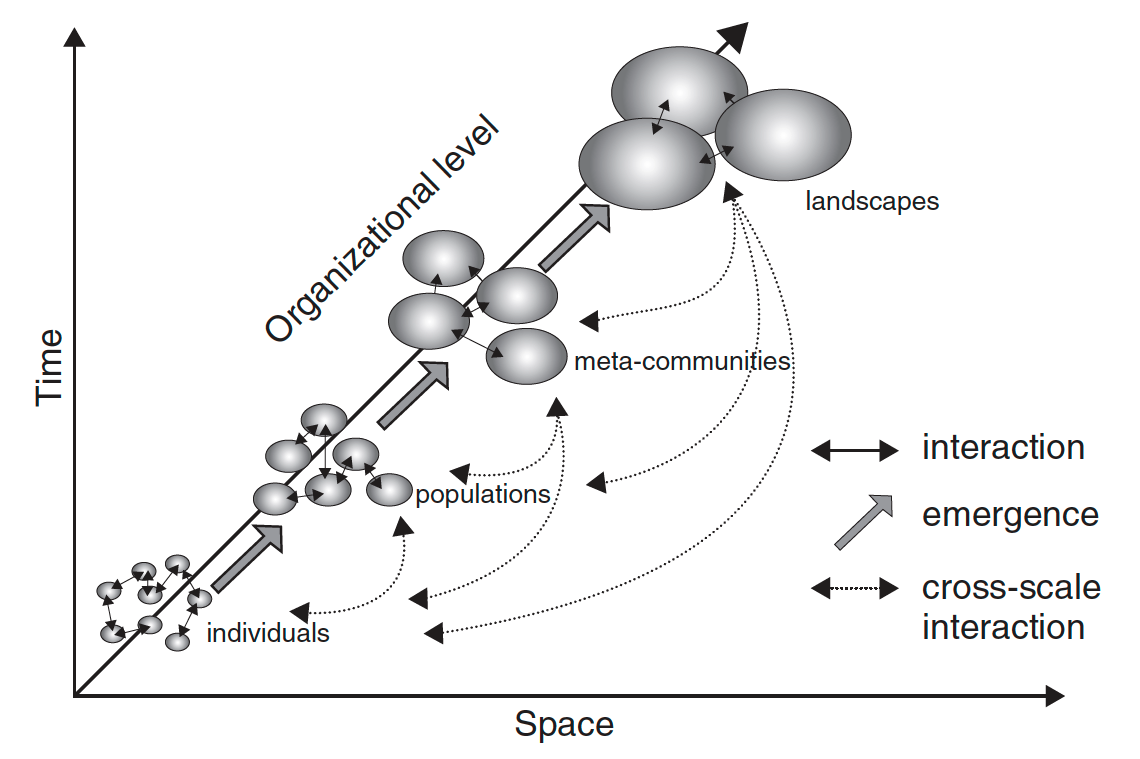
\includegraphics[width=.8\textwidth]{conclusion/figures/complex.png}
\caption[Représentation conceptuelle des effets des changements environnementaux sur les différents niveaux d'organisation biologique]{Représentation conceptuelle des effets des changements environnementaux sur les forêts sous l'angle d'un système complexe. Les changements dans la dynamique des forêts sont transférés de façon ascendante entre les différents niveaux d'organisation biologique. Des interactions et des rétroactions ont lieu entre les entités à l'intérieur et à travers les échelles spatiales, temporelles et hiérarchiques. Les entités qui interagissent à un niveau donnent naissance à des entités émergentes de niveau supérieur, dont l'existence, à son tour, affecte le comportement des entités de niveau inférieur. Schéma issu de Messier \emph{et al.} (2013).}
\label{fig4.2}
\end{figure}

\hypertarget{changements-duxe9mographiques}{%
\subsection{Changements
démographiques}\label{changements-duxe9mographiques}}

Dans un premier temps, le réchauffement climatique favorise le
recrutement, la survie et la croissance des espèces tempérées à leur
limite nord
\citep{fisichelli_temperate_2014, boisvertmarsh_divergent_2019, goldblum_tree_2005, grundmann_impact_2011, bolte_understory_2014},
ce qui leur confère un avantage compétitif par rapport aux espèces
boréales. Mais, en l'absence de perturbations, les arbres poussent
lentement, leurs taux de mortalité et de recrutement sont faibles et la
compétition pour l'espace et la lumière est intense.

Des perturbations peuvent cependant éliminer les individus des espèces
résidentes. Dans la zone d'étude, les perturbations naturelles et
anthropiques ont provoqué une mortalité disproportionnée d'une espèce
dominante dans les forêts mixtes (Chapitre \ref{chap2}). En effet, le
sapin baumier a subi une mortalité massive suite aux grandes épidémies
de tordeuse des bourgeons de l'épinette dans les années 1967-1992
\citep{duchesne_population_2008}. De plus, cette espèce est aussi la
plus coupée au Québec. Suite à une perturbation modérée (e.g., épidémie
légère, coupe partielle), les trouées dans la canopée résultant de la
perte de cette espèce boréale ubiquiste et abondante ont probablement
permis de réduire la compétition et libérer des ressources, favorisant
ensuite la croissance rapide des espèces tempérées compagnes, telles que
les érables rouge et à sucre ainsi que le bouleau jaune (Chapitre
\ref{chap2}). De plus, alors que les perturbations naturelles semblent
avoir un effet plutôt délétère, les coupes partielles favorisent une
hausse du recrutement de ces espèces tempérées à leur limite nord
(Chapitre \ref{chap3}). En cas de perturbations majeures (e.g., grand
feu, coupe totale), la majorité des arbres en place meurent ce qui crée
des ouvertures de très grande superficie. Ces paysages nouvellement
ouverts sont colonisés rapidement par des espèces pionnières (Chapitre
\ref{chap2}) qui peuvent disperser leurs graines sur de longues
distances et croitre rapidement en conditions lumineuses, telles que le
peuplier faux-tremble et le bouleau blanc
\citep{boucher_fire_2017, grondin_have_2018}. Suite à une perturbation
majeure, les espèces tempérées peuvent être plus lentes à revenir parce
qu'elles se dispersent sur des distances plus courtes
\citep{scheller_spatially_2005}.

\hypertarget{dynamique-des-populations}{%
\subsection{Dynamique des populations}\label{dynamique-des-populations}}

Le réchauffement et les perturbations peuvent donc exercer leur
influence sur la dynamique de population des espèces par le biais de
plusieurs processus démographiques, notamment la reproduction, le
recrutement, la croissance et la mortalité. Ces changements à l'échelle
des individus et des sites s'accumulent dans le temps et dans l'espace
pour altérer l'abondance et l'aire de répartition des populations
\citep{holt_theoretical_2005}. Lorsque les effets sur les individus
d'une espèce sont généralement négatifs, le taux de croissance de la
population diminuera; certaines populations pourraient être amenées à
disparaître localement et, dans le pire des cas, régionalement. À
l'inverse, lorsque les effets sur les taux démographiques d'une espèce
sont positifs, les populations grandissent, ce qui peut entraîner une
augmentation locale de l'abondance et une expansion régionale de l'aire
de répartition.

Ces effets sur le fitness des espèces ne sont pas aléatoires, mais sont
déterminés par leurs tolérances physiologiques, leurs stratégies
d'histoire de vie et leurs capacités de dispersion
\citep{aubin_traits_2016, estrada_species_2015}. La diversité des
caractéristiques écologiques spécifiques est sans doute à l'origine de
la grande variabilité dans les réponses des arbres face aux multiples
stresseurs environnementaux \citep{serra-diaz_disturbance_2015}. Alors
que le réchauffement peut favoriser le taux de croissance des
populations d'espèces qui sont limitées par les températures très
froides, les perturbations devraient promouvoir les espèces
opportunistes, intolérantes à l'ombre, avec une bonne capacité de
dispersion et de reproduction végétative \citep[Chapitre
\ref{chap3};][]{de_frenne_microclimate_2013, danneyrolles_stronger_2019}.
Par exemple, l'érable rouge, dont la distribution au nord est en partie
limitée par un faible niveau de reproduction sexuée
\citep{tremblay_potential_2002}, est reconnue comme une espèce
super-généraliste et opportuniste, capable de coloniser rapidement des
sites variés après une perturbation
\citep{abrams_red_1998, fei_rapid_2009}. Ces caractéristiques pourraient
donc expliquer l'expansion rapide qu'a connue l'érable rouge au Québec
sous l'effet combiné du réchauffement et des perturbations (Chapitres
\ref{chap1}, \ref{chap2} et \ref{chap3}). En revanche, certaines espèces
limitées par la dispersion, comme le tilleul d'Amérique, limitées à un
habitat spécifique, comme l'érable argenté, ou encore intolérante aux
perturbations, comme la pruche du Canada, pourraient ne pas bénéficier
des opportunités de recrutement et de croissance suivant des
perturbations, et ce, même si le climat devient plus favorable.

De plus, la sensibilité au climat peut varier entre les différents
processus démographiques \citep{niinemets_responses_2010}. Par exemple,
comme la régénération est souvent plus sensible que la survie des
adultes aux stress hydrique ou thermique
\citep{niinemets_responses_2010}, une population peut persister pendant
des décennies ou des siècles sur un site donné, même si les conditions
climatiques sont devenues défavorables à sa régénération
\citep{talluto_extinction_2017}. Pour cette raison,
\citet{jump_altitude-for-latitude_2009} ont suggéré que l'expansion à la
limite nord de la distribution d'une espèce sera plus rapide que les
changements à la limite sud puisque la reproduction et le recrutement
sont plus sensibles aux changements environnementaux que la mortalité
des individus établis. Dans les forêts du Québec, les données montrent
effectivement une augmentation rapide de l'abondance (Chapitre
\ref{chap1}) et du recrutement des espèces tempérées dominantes
(Chapitre \ref{chap3}). Toutefois, la perte des espèces boréales a sans
doute été tout aussi importante sinon plus puisque la mortalité n'était
pas contrôlée par un stress climatique mais surtout par des
perturbations directes, comme les coupes, les feux et les épidémies
(Chapitres \ref{chap1} et \ref{chap2}). Ainsi, contrairement à
l'hypothèse avancée par \citet{jump_altitude-for-latitude_2009}, les
perturbations risquent d'accélérer la contraction de l'aire de
répartition des espèces boréales, tandis que l'effet sur l'expansion des
espèces tempérées à leur limite nord pourrait être beaucoup plus lent en
raison des contraintes au recrutement (Chapitre \ref{chap3}). En effet,
le recrutement des espèces tempérées est largement dépendant de la
présence des arbres matures conspécifiques pour la dispersion et est
freiné par la compétition des espèces boréales de même que par les
conditions de mauvais drainage (sites hydriques) dans les bas de pente
(Chapitre \ref{chap3}).

\hypertarget{dynamique-des-communautuxe9s}{%
\subsection{Dynamique des
communautés}\label{dynamique-des-communautuxe9s}}

Les changements démographiques des espèces se traduisent donc en pertes
et en gains d'espèces à l'échelle locale qui influencent la composition
et la structure des communautés forestières. Dans l'écotone
boréal-tempéré, la thermophilisation des forêts résultait principalement
du gain d'une seule espèce tempérée, l'érable rouge, combiné à la perte
de deux espèce boréales dominantes, le sapin et l'épinette noire, et ce
phénomène était accentué par les perturbations modérées (Chapitre
\ref{chap1}). Ainsi, sans perturbation, le renouvellement de la
communauté est très lent, tandis que celui-ci est accéléré par les
perturbations modérées (Chapitres \ref{chap1}, \ref{chap2} et
\ref{chap3}). En revanche, les perturbations majeures détruisent la
communauté en place et réinitialisent la succession à partir du début
entraînant surtout des gains en espèces pionnières (Chapitres
\ref{chap1} et \ref{chap2}). Au cours de ma thèse, j'ai pu montrer
comment ces changements de composition résultent de l'action conjointe
de trois mécanismes démographiques qui altèrent la trajectoire de
succession après une perturbation modérée: (1) la mortalité d'une espèce
dominante; (2) le relâchement de la croissance des espèces tempérées
compagnes; et (3) le recrutement accru des gaulis des espèces tempérées
compagnes ou présentes dans le voisinage.

Les conséquences au niveau des communautés des changements d'aires de
répartition spécifiques aux espèces pourraient mener à la formation de
communautés sans analogues, i.e.~des communautés dans lesquelles
coexistent des espèces dans des combinaisons historiquement inconnues
\citep{williams_novel_2007}. Les modèles de distribution d'espèces sous
l'effet du changement climatique prédisent un grand potentiel
d'augmentation de la richesse au Québec
\citep{berteaux_changements_2014}. Toutefois, mes résultats soulignent
que seul une poignée d'espèces tempérées prospèrent sous ce nouveau
régime de perturbations anthropiques. Par conséquent, il est fort
probable que les forêts de l'écotone ne connaîtront pas un
enrichissement, mais plutôt un appauvrissement associé à l'expansion
d'une ou quelques espèces. On prévoit en outre que le déclin des espèces
boréales actuellement dominantes, soit le sapin et l'épinette, risque de
s'accentuer dans les prochaines décennies dans les domaines de la
sapinière en raison du réchauffement climatique
\citep{dorangeville_beneficial_2018}. Le remplacement de ces espèces
résineuses par des espèces feuillues pourrait avoir des conséquences
économiques importantes. Par exemple, l'expansion de l'érable rouge
pourrait compromettre l'approvisionnement en espèces résineuses à grande
valeur commerciale dans la forêt mixte. De plus, les pratiques
sylvicoles devront être révisées pour s'adapter à la nouvelle réalité
puisqu'elles sont élaborées en fonction de la composition et de la
dynamique naturelle des forêts et dépendent de la régénération naturelle
\citep{pinna_amenagement_2009}.

\hypertarget{duxe9placement-des-grands-biomes-forestiers}{%
\subsection{Déplacement des grands biomes
forestiers}\label{duxe9placement-des-grands-biomes-forestiers}}

Les effets cumulés des changements à l'échelle des individus, des
populations et des communautés, peuvent finalement entraîner un
déplacement des grands biomes forestiers à l'échelle régionale,
notamment une expansion de la forêt tempérée au détriment de la forêt
mixte (Chapitre \ref{chap2}). Cette réorganisation régionale de la
composition des forêts peut interagir avec le fonctionnement des
écosystèmes à l'échelle locale et les processus à l'échelle globale
\citep[\emph{cross-scale interaction};][]{peters_crossscale_2007}. Ces
changements de fonctionnement risquent d'être d'autant plus grand à
l'écotone puisque les espèces feuillues et les espèces résineuses
présentent des différences importantes sur le plan de leurs
caractéristiques et fonctions écologiques
\citep{wardle_terrestrial_2011}. L'enfeuillement des forêts mixtes
pourrait par exemple influencer localement la qualité de la litière, le
taux de décomposition de la matière organique et la composition des
microorganismes du sol
\citep{laganiere_how_2010, legare_influence_2005}. Les changements dans
la composition, la structure d'abondance et la distribution spatiale des
forêts affecteront également la survie et la distribution des nombreuses
espèces de mammifères, d'oiseaux et d'insectes qui en dépendent pour
s'abriter et se nourrir \citep{friggens_effects_2018}. Comme les espèces
feuillues sont moins inflammables et moins sensibles aux insectes
ravageurs que les conifères, leur augmentation dans le paysage forestier
peut modifier le régime régional de perturbations
\citep{terrier_potential_2013, mffp_insectes_2018}. À long terme,
l'expansion du biome tempéré au détriment des forêts mixtes et des
forêts boréales pourrait avoir un effet sur le climat global en
augmentant la séquestration du carbone \citep{thurner_carbon_2014} ainsi
que l'albédo \citep{anderson_biophysical_2011}.

\hypertarget{les-perturbations-catalyseurs-de-changements-dans-les-foruxeats}{%
\section{Les perturbations --- catalyseurs de changements dans les
forêts}\label{les-perturbations-catalyseurs-de-changements-dans-les-foruxeats}}

Les effets combinés du changements climatiques et des perturbations
peuvent donner naissance à des dynamiques non-linéaires, comme un
changement de régime écologique \citep[Fig.
\ref{fig4.2};][]{scheffer_catastrophic_2001, harris_biological_2018}. Un
changement de régime résulte d'une réorganisation rapide de la
composition et de la structure d'un écosystème qui entraîne un
basculement vers un nouvel état alternatif stable
\citep{scheffer_catastrophic_2001}. Par exemple, si la transition des
forêts mixtes vers des forêts à dominance tempérée documentée dans le
Chapitre \ref{chap2} persiste, cette transformation pourrait bel et bien
s'avérer être un changement de régime.

En théorie, des changements d'états stables peuvent subvenir suivant
deux mécanismes: (1) des changements graduels dans les conditions
environnementales jusqu'à un niveau critique auquel le système
s'effondre soudainement, et (2) des perturbations trop sévères ou en
rafale qui poussent le système hors de son bassin d'attraction
\citep{scheffer_catastrophic_2001}. Par exemple, la grande augmentation
des taux de mortalité des arbres dans l'ouest des États-Unis en réponse
à un stress hydrique grandissant \citep{van_mantgem_apparent_2007}
pourrait être le signe avant-coureur d'un dépérissement massif des
forêts. Dans un autre cas, \citet{payette_shift_2003} a montré que les
impacts cumulés de la coupe forestière, suivie d'une épidémie d'insectes
puis d'un incendie pourraient avoir des effets catastrophiques sur la
régénération des arbres, entraînant la transition d'une pessière dense
en un milieu ouvert dominé par le lichen. Bien que les deux mécanismes
puissent indépendamment mener à une transition rapide d'état, leurs
effets synergiques augmentent le risque de changements rapides de régime
écologique \citep{scheffer_catastrophic_2001, harris_biological_2018}.
Mes résultats supportent cette hypothèse et suggèrent que les forêts
répondent à l'effet cumulé d'un stress à long terme causé par le
changement climatique (i.e., \emph{press disturbance}), en combinaison
avec des événements de mortalités aiguës \citep[i.e., \emph{pulse
disturbance};][]{harris_biological_2018}. Ainsi, le réchauffement
climatique érode la résilience des forêts mixtes tandis que les
perturbations éliminent les espèces boréales en place et accélèrent le
processus de succession vers davantage d'espèces tempérées adaptées aux
températures plus chaudes (Chapitres \ref{chap1}, \ref{chap2} et
\ref{chap3}).

\hypertarget{ruxe9silience-uxe9tats-alternatifs-stables-et-changement-de-ruxe9gime}{%
\subsection{Résilience, états alternatifs stables et changement de
régime}\label{ruxe9silience-uxe9tats-alternatifs-stables-et-changement-de-ruxe9gime}}

Les résultats issus de ma thèse m'ont amenée à réfléchir en profondeur à
la dynamique de changement de régime dans le contexte de l'écotone
boréal-tempéré et à redéfinir le paysage conceptuel des états stables de
cette région (Fig. \ref{fig4.1}). Le long du gradient latitudinal, la
forêt boréale au nord et la forêt tempérée au sud sont les seuls états
stables possibles (Fig. \ref{fig4.1}a). Ces états forestiers ont une
grande résilience face aux perturbations de type \emph{pulse} qui sont
dans la plage de variabilité naturelle de leur région
\citep{grondin_have_2018}; une perturbation naturelle ou anthropique
peut déplacer le système à l'intérieur du bassin d'attraction, mais le
système peut ensuite se rétablir et revenir à son état initial.

Dans la zone de transition entre ces deux grands biomes, on trouve la
forêt mixte, un état relativement rare qui change facilement d'un état
de dominance à un autre (Fig. \ref{fig4.1}a). Ceci suggère que la forêt
mixte ne serait pas l'état stable de la région, mais que cette
communauté représente plutôt un état instable où le système n'est que
transitoire. La coexistence des espèces boréales, tempérées et
pionnières dans la forêt mixte est maintenue grâce à l'hétérogénéité des
perturbations naturelles combinée à des différences dans les stratégies
de cycle de vie des espèces
\citep{kneeshaw_natural_2007, bouchard_tree_2006} sous un climat donné.

En plus des perturbations de type \emph{pulse}, le climat global change
graduellement et de façon persistante, ce qui peut altérer la forme du
paysage des états stables (Fig. \ref{fig4.1}b). À mesure que le climat
se réchauffe, les forêts peuvent perdre leur capacité à se rétablir
puisque les espèces en place ne sont plus aussi bien adaptées au climat
\citep{johnstone_changing_2016}. Mon interprétation est que le
réchauffement modifie surtout le bassin d'attraction de l'état mixte et
abaisse le seuil critique à franchir pour se rendre à l'état tempéré
(Fig. \ref{fig4.1}b). De plus, le réchauffement peut rendre le bassin de
l'état tempéré plus large et profond, donc plus attractif, et,
inversement, celui de l'état boréal moins profond. Ces modifications de
la courbe des états alternatifs stables fragilisent la forêt mixte,
mais, en l'absence de perturbation, la grande inertie des forêts cache
la perte de résilience de l'état mixte. Les arbres, ayant une longue
durée de vie, peuvent faire paraître les forêts inébranlables face aux
changements environnementaux même si la niche de régénération est en
train de se déplacer
\citep{sittaro_tree_2017, boisvertmarsh_divergent_2019}. Toutefois, une
perturbation peut facilement faire basculer le système vers un nouvel
état; la composition des forêts mixtes peut donc se déplacer rapidement
vers une dominance en espèces tempérées qui sont mieux adaptées aux
températures plus chaudes.

\newpage

\begin{figure}
\centering
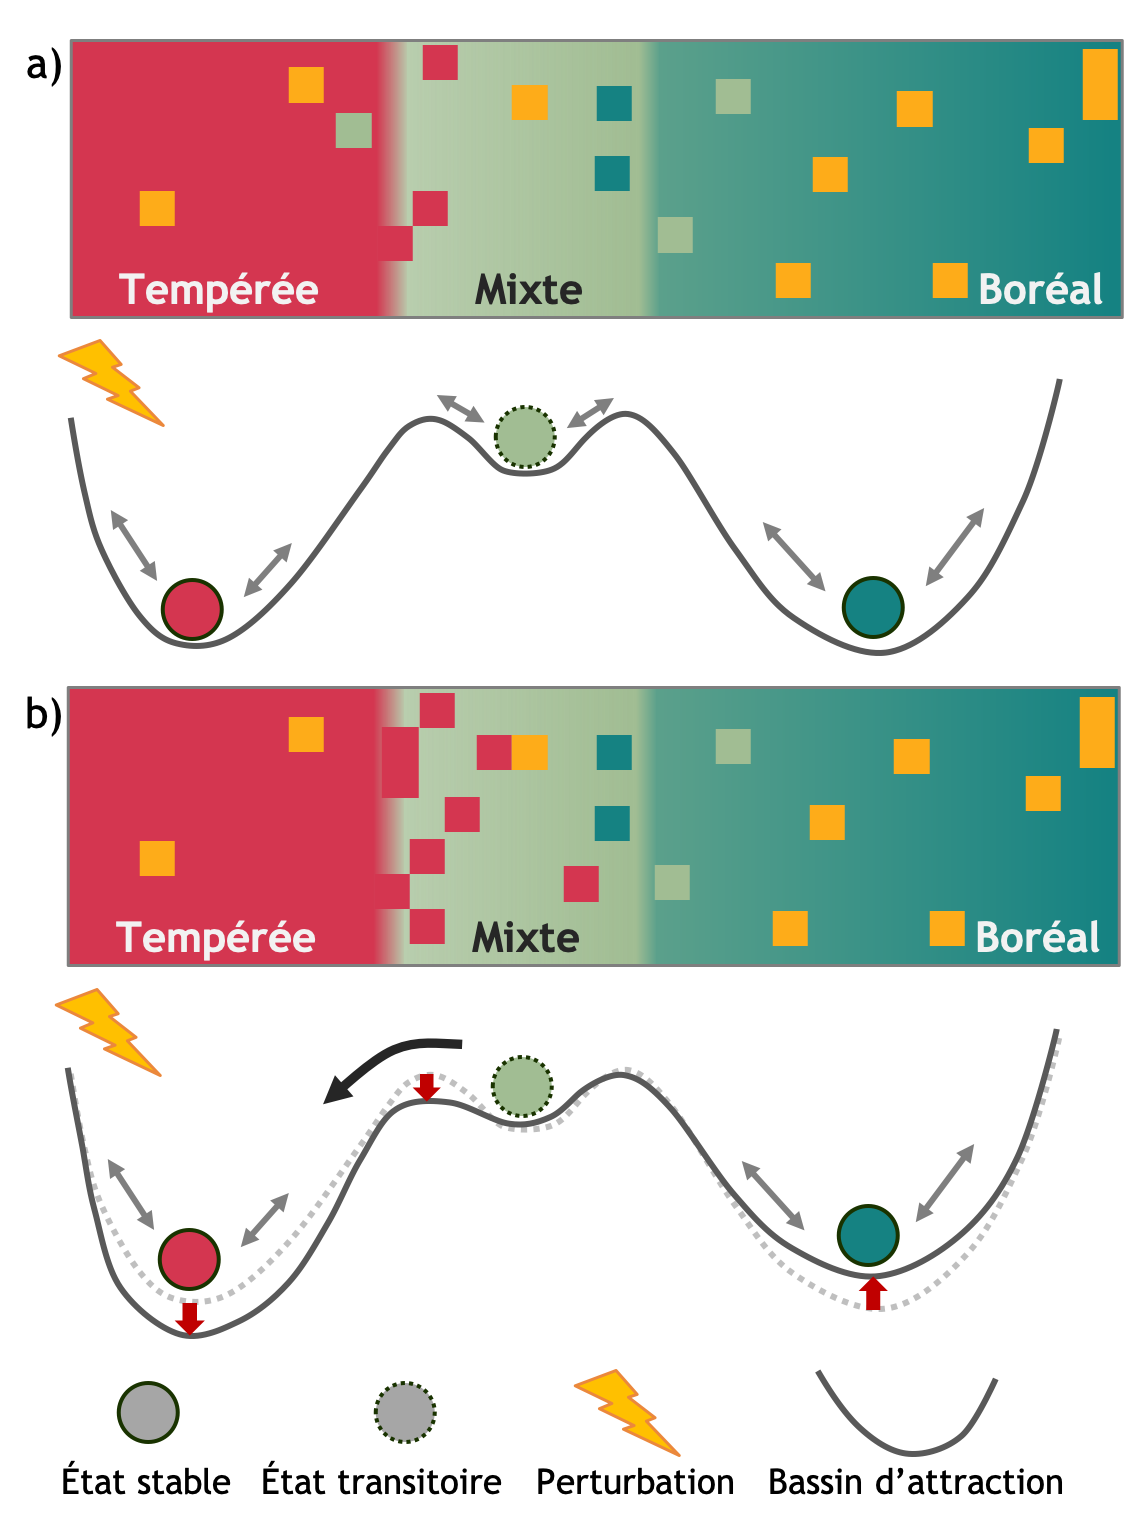
\includegraphics[width=.63\textwidth]{conclusion/figures/etat_alternatif2.png}
\caption[Représentation conceptuelle des états alternatifs stables le long du gradient latitudinal]{Nouvelle représentation conceptuelle des états alternatifs stables le long du gradient latitudinal sans changement climatique (a) et avec changement climatique (b). Dans le schéma avec la courbe, la boule caractérise l'état de l'écosystème à un instant donné, la courbe correspond à l'ensemble des états dans lesquels l’écosystème peut se retrouver, les vallées sont les bassins d'attraction des équilibres stables, et les sommets des collines sont les équilibres instables. Le schéma rectangulaire représente le paysage correspondant. Au sud du gradient latitudinal au de température, un seul état stable existe, la forêt tempérée (en rouge). Au nord du gradient, l'état stable dominant est la forêt boréale (en bleu). Ce sont des états stables dynamiques; les perturbations peuvent faire déplacer la boule dans son bassin d'attraction et elle peut même passer par l'état pionnier (un état transitoire non représenté sur la courbe, mais représenté par des carrés jaunes dans le paysage). La forêt étant habituellement résiliente aux perturbations, elle retourne ensuite vers son état initial. Au centre, dans l'écotone, la forêt mixte (en vert) serait un état transitoire entre les deux états stables dominants qui est maintenue grâce à la dynamique naturelle de perturbations. Le changement du climat (b) peut provoquer un changement de la forme du paysage de différentes façons: (1) en abaissant le seuil pour passer de l'état mixte à tempéré, (2) en creusant et en élargissant le bassin d'attraction de l'état tempéré et (3) en rendant moins profond le bassin d'attraction de l'état boréal. Ces modifications font que la boule dégringole plus souvent de la vallée mixte vers la vallée tempérée sous l'effet d'une perturbation.}
\label{fig4.1}
\end{figure}

Contrairement aux perturbations modérées, les perturbations majeures
détruisent toutes la communauté en place et poussent le système vers
l'état pionnier, i.e. des peuplements dominés par des espèces
intolérantes à l'ombre ou bien avec pas ou très peu d'arbres (Chapitre
\ref{chap2}). Leur effet à long terme est difficile à prévoir à partir
des données d'inventaire puisque les systèmes n'ont sans doute pas eu le
temps de revenir à un état stable. En effet, l'état pionnier est en
général un état transitoire. Il est donc fort probable que la majorité
des forêts soient encore en train de se déplacer vers leur état
d'équilibre. Toutefois, il se pourrait que certaines forêts se soient
transformées définitivement. Par exemple, les peuplements de peuplier
faux-tremble dans les pessières noires représentent normalement un état
de transition, mais, sous l'effet des coupes forestières, ces
peuplements sont en expansion et semblent se maintenir
\citep{grondin_les_2003}.

La fréquence et la gravité des perturbations naturelles, telles que les
incendies, les épidémies d'insectes, les sécheresses et les vagues de
chaleur, devraient augmenter dans de nombreuses régions du monde
\citep{seidl_forest_2017, bergeron_past_2006}. À la lumière de mes
résultats, cela pourrait conduire à des changements majeurs dans la
composition des forêts au cours des prochaines décennies et
potentiellement à des modifications permanentes des états forestiers.
Cependant, si les perturbations deviennent trop fréquentes et trop
intenses, les forêts pourraient basculer vers une dominance en espèces
pionnières de début de succession. Des comportements non-linéaires dans
les réponses des écosystèmes forestiers impliquent que de nombreuses
projections sous-estiment probablement l'ampleur des changements futurs
de la biodiversité \citep{scheffer_catastrophic_2001}. Une telle
conclusion souligne l'importance de tenir compte de l'effet synergique
des perturbations et du changement climatique dans les stratégies de
gestion forestière ainsi que dans les modèles de prédiction.

\hypertarget{lamuxe9nagement-forestier-dans-un-monde-en-changement-et-incertain}{%
\section{L'aménagement forestier dans un monde en changement et
incertain}\label{lamuxe9nagement-forestier-dans-un-monde-en-changement-et-incertain}}

Les effets multiples des changements globaux sur la dynamique forestière
soulèvent un défi majeur pour l'aménagement de nos forêts. Face à la
rapidité et à l'incertitude de ces changements, nos pratiques visant à
contrôler et prédire l'évolution de nos forêts risquent d'être
contreproductive \citep{puettmann_critique_2009}. Étant donné que les
coupes forestières ont une influence majeure sur la composition
(Chapitre \ref{chap1}), la dynamique (Chapitre \ref{chap2}) et la
régénération des forêts (Chapitre \ref{chap3}) et interagissent avec le
changement du climat, il est évident que les futures politiques
d'aménagement auront un rôle fondamental à jouer pour aider les forêts à
s'adapter rapidement et faire face aux changements globaux.

Le réchauffement que nous avons connu jusqu'à présent n'est que mineur
par rapport à ce qui est attendu d'ici la fin du siècle. Néanmoins, tel
que mis en évidence dans l'ensemble de ma thèse, de grandes
transformations sont déjà évidentes à toutes les échelles de
l'organisation biologique. Avec l'accélération des changements
environnementaux et l'inertie inhérente de la dynamique forestière, le
déséquilibre ne pourra que s'accentuer et les réponses des forêts
dépendront des dynamiques transitoires déjà en cours. Actuellement, les
principes fondamentaux de l'estimation de la productivité des
peuplements forestiers reposent sur des taux de mortalité et de
croissance prévisibles sous un climat constant. En aménagement
forestier, on présume que le climat est stable et que les forêts sont à
équilibre. À court terme, ces hypothèses sont valables. Mais, à long
terme, elles sont particulièrement problématiques dans le contexte du
changement climatique. En effet, comme la dynamique forestière n'est pas
à l'équilibre \citep{talluto_extinction_2017}, la trajectoire de
succession et la niche de régénération sont facilement altérées sous
l'effet combiné du réchauffement et des perturbations (Chapitres
\ref{chap2} et \ref{chap3}). Les prédictions issues de calculs qui
supposent l'équilibre pourraient à la fois sur-estimer la capacité de
régénération et de croissance de certaines espèces et sous-estimer la
mortalité associée à des extrêmes climatiques, menant ainsi à une
planification mal adaptée. Par conséquent, les activités de gestion
doivent non seulement anticiper le changement, mais aussi reconnaître
que les systèmes actuels ont déjà été transformés et sont en train de se
transformer davantage. L'importance de ce point a été bien exprimée par
\citet{seastedt_management_2008} :

\begin{quote}
In managing novel ecosystems, the point is not to think outside the box
but to recognize that the box has moved, and in the 21st century, the
box will continue to move more rapidly.
\end{quote}

\hypertarget{uxe9volution-de-lamuxe9nagement-au-quuxe9bec}{%
\subsection{Évolution de l'aménagement au
Québec}\label{uxe9volution-de-lamuxe9nagement-au-quuxe9bec}}

Une importante volonté de gestion durable des forêts s'est développée
dans les dernières décennies à travers le monde. Jusqu'à la fin du
XX\textsuperscript{e} siècle, les modèles de gestion ont une vision
utililariste de la forêt et sont centrés sur la production
\citep{kuuluvainen_natural_2012}. Depuis les années 1990, la foresterie
a évolué vers un aménagement qui intègre davantage de critères
écologiques et sociaux \citep{messier_managing_2013}. Au Québec, dans la
foulée du documentaire \emph{L'erreur boréale}, sorti en 1999, une
grande réflexion s'est amorcée sur l'exploitation de la forêt publique.
Pour répondre aux inquiétudes de la population, la Commission d'étude
sur la gestion de la forêt publique québécoise est formée en 2003 et
dépose un rapport en 2004 qui fait état de la situation et formule de
nombreuses recommandations pour améliorer et moderniser la gestion des
forêts
\citep{commission_detude_sur_la_gestion_de_la_foret_publique_quebecoise_commission_2004}.
En réponse à ces recommandations, le Québec se dote de la Loi sur
l'aménagement durable du territoire forestier, en vigueur depuis 2013,
qui promeut un aménagement écosystémique. L'aménagement écosystémique
s'inspire des patrons spatio-temporels générés par les perturbations
naturelles, qui servent d'états de référence, afin de maintenir les
écosystèmes dans leur plage de variabilité naturelle historique, et
ainsi réduire les écarts entre la forêt naturelle et aménagée
\citep{vaillancourt_implementation_2009, attiwill_disturbance_1994}.

L'aménagement écosystémique représente une grande avancée car il intègre
un ensemble d'objectifs sociaux et écologiques plus larges et reconnait
l'importance de la biodiversité et des processus écologiques qui
influencent la dynamique forestière
\citep{messier_functional_2019, kuuluvainen_forest_2009}. Cette nouvelle
approche de gestion présente néanmoins une lacune majeure; ces pratiques
de gestion ne sont pas conçues pour faire face au rythme rapide des
changements globaux et à l'incertitude croissante qui en découle
\citep{messier_dealing_2016, millar_climate_2007}. En effet, des
pratiques de gestion qui visent à maintenir la composition et la
structure des forêts historiques de référence vont devenir de plus en
plus difficile à mettre en oeuvre
\citep{duveneck_measuring_2016, boulanger_climate_2019} et ne permettent
pas nécessairement d'améliorer la capacité des écosystèmes à s'adapter à
un nouvel ensemble de conditions environnementales
\citep{seastedt_management_2008}. Bien que l'utilisation stricte des
conditions de référence historiques deviendra contre-productive en tant
qu'objectifs spécifiques, les informations historiques documentant la
dynamique naturelle des écosystèmes forestiers seront essentielles pour
mieux appréhender les dynamiques du futur
\citep{harris_ecological_2006}.

\hypertarget{amuxe9nager-les-foruxeats-pour-augmenter-leur-ruxe9silience-et-leur-capacituxe9-adaptative}{%
\subsection{Aménager les forêts pour augmenter leur résilience et leur
capacité
adaptative}\label{amuxe9nager-les-foruxeats-pour-augmenter-leur-ruxe9silience-et-leur-capacituxe9-adaptative}}

La solution privilégiée pour faire face au changement climatique est
d'accroître la résilience et la capacité adaptative des forêts
\citep{messier_managing_2013, seastedt_management_2008}. Alors que la
résilience permet à une forêt de retrouver sa structure et ses fonctions
d'origine, la capacité adaptative lui permet de diverger d'un état
antérieur qui était mal adapté aux conditions environnementales
\citep{messier_managing_2013, filotas_viewing_2014}. Les perturbations
naturelles et les variations climatiques sont inévitables mais en
développant une grande diversité, les forêts auront les outils
nécessaires pour se réorganiser et s'adapter à des conditions futures
sans précédent \citep{messier_dealing_2016}. S'appuyant sur l'hypothèse
d'assurance \citep[de l'anglais \emph{insurance
hypothesis};][]{yachi_biodiversity_1999}, l'idée est de favoriser la
diversité génétique, spécifique, fonctionnelle et structurale dans les
forêts afin d'augmenter les chances que certaines espèces continueront à
assurer le fonctionnement de l'écosystème même si d'autres
disparaissent.

Pour favoriser la capacité adaptative des forêts, il faut avant tout
maintenir la diversité naturelle que l'on trouve à toutes les échelles
spatiales, du peuplement jusqu'au biome, de manière à garder les options
d'adaptation qui existent déjà. Par exemple, bien que peu résilientes,
les forêts mixtes du Québec ont montré une bonne capacité adaptative
face au changement climatique puisqu'elles ont réussi se réorganiser de
manière à ajuster leur composition aux nouvelles conditions
environnementales. En effet, suite à une perturbation, des trajectoires
diversifiées peuvent émerger dans les peuplements mixtes puisqu'ils
présentent une hétérogénéité en termes de structure, d'âge, de tolérance
physiologique et de stratégies d'histoire de vie.

Dans d'autres cas, il sera peut-être nécessaire de cultiver activement
la capacité adaptative des écosystèmes grâce à l'aménagement. Ce
principe pourrait devenir important dans les forêts boréales étant donné
leur composition très homogène et leur très grande inertie face au
changement climatique. En effet, alors qu'il y a eu très peu de
transitions vers l'état mixte et pas de thermophilisation des
communautés, on a plutôt observé une dynamique de remplacement entre les
états pionnier et boréal (Chapitres \ref{chap1} et \ref{chap2}). Comme
les forêts du nord du Québec sont très pauvres en espèces, étant
largement dominées par l'épinette noire et le sapin baumier, elles ont
moins de ressources que les forêts mixtes pour faire face aux
changements récents et futurs, ce qui pourrait limiter leur capacité à
s'ajuster et s'éloigner d'un état possiblement mal adapté. De plus, on
prévoit que le climat de la forêt boréale de l'est de l'Amérique du Nord
devrait ressembler à celui de la forêt tempérée d'ici la fin du siècle
\citep{gauthier_boreal_2015}. Toutefois, la migration des espèces
tempérées dans ces régions semble limitée par plusieurs facteurs
non-climatiques, notamment leur capacité de dispersion, la compétition
par les espèces boréales, ainsi que les conditions édaphiques
\citep[Chapitre
\ref{chap3};][]{solarik_priority_2019, carteron_soil_2020}. Les
plantations d'enrichissement pourraient alors s'avérer nécessaires pour
faciliter la migration des espèces tempérées vers le nord et assurer la
résilience des forêts \citep{duveneck_measuring_2016}. Par exemple, tel
que suggéré pour la migration postglaciaire des arbres
\citep{mclachlan_molecular_2005}, les populations aujourd'hui marginales
pourraient jouer un rôle très important dans la migration future des
arbres en réponse au changement climatique (Chapitre \ref{chap3}).
Ainsi, la création d'îlots de forêts mixtes sur les sommets de collines
dans les forêts boréales assurerait la présence de semenciers de
différentes espèces capables de coloniser rapidement les sites après
perturbation lorsque les conditions climatiques seront adéquates.
Finalement, étant donné les interactions entre échelles, les changements
de régime écologique et la variabilité des réponses des espèces, il
devient de plus en plus clair qu'on ne peut forcer un peuplement à se
développer dans une direction précise prédéterminée en fonction de nos
besoins en bois \citep{puettmann_critique_2009}. Des recherches récentes
encouragent donc à revoir la planification de façon à avoir des
objectifs plus larges et plus flexibles qui permettent un ensemble de
différentes trajectoires futures à l'échelle régionale
\citep{messier_dealing_2016, puettmann_critique_2009}.

Cette idée de favoriser la diversité pour assurer la résilience est déjà
prise en compte dans l'aménagement écosystémique et constitue donc une
porte d'entrée à l'adaptation aux changements climatiques
\citep{samuel_foret_2011}. Toutefois, il faut éviter de mettre tous nos
oeufs dans le même panier. Les modèles de projections climatiques nous
ont informé d'un risque croissant de vagues de chaleur et de sécheresses
\citep{ipcc_climate_2014}. Par conséquent, il apparaît logique de mettre
l'emphase sur la promotion des espèces qui résistent à la sécheresse.
Mais, dans un contexte d'incertitude, cette stratégie ne suffit pas
puisqu'il est possible que ce ne soit pas la sécheresse qui causera le
plus grand stress aux forêts, mais plutôt l'augmentation de la fréquence
des feux, l'arrivée de nouveaux insectes ravageurs ou encore les
variations de températures printanières. De plus, tel que montré dans
cette thèse, tous ces facteurs de risque peuvent interagir entre eux et
mener à des changements rapides et inattendus des écosystèmes
forestiers. La grande incertitude associée aux prédictions des effets
attendus des changements climatiques doit être intégrée dans la gestion
forestière de façon à prendre en compte du large éventail de
vulnérabilités \citep{messier_dealing_2016}. Pour permettre à
l'écosystème de résister ou s'adapter à ces multiples facteurs de
stress, les politiques de sélection des espèces d'arbres pourraient, par
exemple, promouvoir le mélange d'espèces ayant des caractéristiques
fonctionnelles diverses, allant des tolérances physiologiques (aux feux,
aux ravageurs, à la sécheresse), aux différents modes de régénération
(e.g., banque de graines, cônes sérotineux, reproduction végétative)
\citep{messier_functional_2019, puettmann_critique_2009}.

\hypertarget{au-deluxe0-des-foruxeats-aplanir-la-courbe-du-changement-climatique}{%
\section{Au-delà des forêts --- Aplanir la courbe du changement
climatique}\label{au-deluxe0-des-foruxeats-aplanir-la-courbe-du-changement-climatique}}

Au cours des dernières décennies, l'ouest du Canada a subi une épidémie
sans précédent de dendroctone du pin ponderosa, une grave sécheresse
(2001-2003) et des saisons de feux extrêmes. Les effets synergiques de
ces perturbations ont entraîné un dépérissement rapide et extensif des
forêts \citep{williamson_climate_2009}. De telles catastrophes
naturelles en rafales montrent que la capacité des gouvernements à
s'adapter et à contrôler les dommages peut rapidement être excédée. Or,
les prédictions annoncent une accélération de la fréquence et de la
sévérité des événements climatiques extrêmes \citep{ipcc_climate_2014}.
Si nous n'agissons pas maintenant pour décarboniser notre économie et
changer la trajectoire dangereuse dans laquelle nous nous dirigeons, le
climat mondial continuera de se dérégler et la multiplication des
événements climatiques extrêmes dépassera la capacité des systèmes
naturels et humains à se rétablir après des perturbations
\citep{ipcc_summary_2018}. Ainsi, sans mesures d'atténuation du
changement climatique, les stratégies d'aménagement visant à augmenter
la résilience et la capacité adaptative des écosystèmes risquent de
s'avérer vaines. Le récent rapport spécial du GIEC a conclu que limiter
le réchauffement climatique à 1.5 \(^{\circ}\)C est possible mais
exigera des transitions rapides et radicales dans tous les aspects de la
société \citep{ipcc_summary_2018}.

Au cours des premiers mois de 2020, le monde entier a fait face à la
pandémie de COVID-19 et les gouvernements ont adopté des mesures
draconiennes pour tenter d'en atténuer les conséquences. Le message a
été clair: il fallait ralentir le rythme de propagation de la maladie
pour ``aplanir la courbe'' et éviter de dépasser la capacité des
hôpitaux à traiter les malades. Ce même concept s'applique également à
la crise climatique: limiter le réchauffement climatique permettrait de
ne pas dépasser la capacité de support de la Terre et donnerait aux
sociétés et aux écosystèmes une plus grande marge de manoeuvre pour
s'adapter. La réponse des gouvernements et de la population à la
pandémie de COVID-19 nous a montré que nous pouvons agir rapidement et
mettre la santé des individus devant celle de l'économie. Toutefois,
cette crise sanitaire souligne aussi qu'il serait préférable d'adopter
des mesures préventives afin d'atténuer le changement climatique plutôt
que d'attendre passivement de frapper un mur et d'être forcé de vivre
dans l'état d'urgence. Maintenant que nous comprenons de mieux en mieux
les conséquences de l'inaction, la priorité est d'utiliser l'ensemble de
nos connaissances scientifiques pour construire un scénario positif et
durable pour le futur \citep{bennett_bright_2016}. Ainsi, comme l'a
écrit Antoine de Saint-Exupéry dans Citadelle:

\begin{quote}
Pour ce qui est de l'avenir, il ne s'agit pas de le prévoir, mais de le
rendre possible.
\end{quote}


 %\cleardoublepage


% \bibliographystyle{abbrvnat}
% \bibliographystyle{plain-fr}
\bibliographystyle{apalike-uqam}
\bibliography{references.bib}


 % Pour les annexes :


 % Les annexes se font comme les chapitres. Le fichier
 % commence par \francais ou \anglais et ensuite
 % \chapter{..}. Le reste est parreil à un chapitre normal.
%%%%%%%%%%%%%%%%%%%%%%%%%%%%%%%%%%%%%%%%%%%%%%%%%%%%%%%%%%%%
%%%%%%%%%%%%%%%%%%%%                   %%%%%%%%%%%%%%%%%%%%%
%%%%%%%%%%%%%%%%%%%%   A N N E X E     %%%%%%%%%%%%%%%%%%%%%
%%%%%%%%%%%%%%%%%%%%                   %%%%%%%%%%%%%%%%%%%%%
%%%%%%%%%%%%%%%%%%%%%%%%%%%%%%%%%%%%%%%%%%%%%%%%%%%%%%%%%%%%

%%%%%% Annexe article 1 %%%%

\appendix

\renewcommand\thefigure{A.\arabic{figure}}
\renewcommand\thetable{A.\arabic{table}}

% Options for packages loaded elsewhere
\PassOptionsToPackage{unicode}{hyperref}
\PassOptionsToPackage{hyphens}{url}
%
\documentclass[
]{article}
\usepackage{lmodern}
\usepackage{amssymb,amsmath}
\usepackage{ifxetex,ifluatex}
\ifnum 0\ifxetex 1\fi\ifluatex 1\fi=0 % if pdftex
  \usepackage[T1]{fontenc}
  \usepackage[utf8]{inputenc}
  \usepackage{textcomp} % provide euro and other symbols
\else % if luatex or xetex
  \usepackage{unicode-math}
  \defaultfontfeatures{Scale=MatchLowercase}
  \defaultfontfeatures[\rmfamily]{Ligatures=TeX,Scale=1}
\fi
% Use upquote if available, for straight quotes in verbatim environments
\IfFileExists{upquote.sty}{\usepackage{upquote}}{}
\IfFileExists{microtype.sty}{% use microtype if available
  \usepackage[]{microtype}
  \UseMicrotypeSet[protrusion]{basicmath} % disable protrusion for tt fonts
}{}
\makeatletter
\@ifundefined{KOMAClassName}{% if non-KOMA class
  \IfFileExists{parskip.sty}{%
    \usepackage{parskip}
  }{% else
    \setlength{\parindent}{0pt}
    \setlength{\parskip}{6pt plus 2pt minus 1pt}}
}{% if KOMA class
  \KOMAoptions{parskip=half}}
\makeatother
\usepackage{xcolor}
\IfFileExists{xurl.sty}{\usepackage{xurl}}{} % add URL line breaks if available
\IfFileExists{bookmark.sty}{\usepackage{bookmark}}{\usepackage{hyperref}}
\hypersetup{
  pdftitle={Supplementary Information},
  hidelinks,
  pdfcreator={LaTeX via pandoc}}
\urlstyle{same} % disable monospaced font for URLs
\usepackage[margin=1in]{geometry}
\usepackage{longtable,booktabs}
% Correct order of tables after \paragraph or \subparagraph
\usepackage{etoolbox}
\makeatletter
\patchcmd\longtable{\par}{\if@noskipsec\mbox{}\fi\par}{}{}
\makeatother
% Allow footnotes in longtable head/foot
\IfFileExists{footnotehyper.sty}{\usepackage{footnotehyper}}{\usepackage{footnote}}
\makesavenoteenv{longtable}
\usepackage{graphicx,grffile}
\makeatletter
\def\maxwidth{\ifdim\Gin@nat@width>\linewidth\linewidth\else\Gin@nat@width\fi}
\def\maxheight{\ifdim\Gin@nat@height>\textheight\textheight\else\Gin@nat@height\fi}
\makeatother
% Scale images if necessary, so that they will not overflow the page
% margins by default, and it is still possible to overwrite the defaults
% using explicit options in \includegraphics[width, height, ...]{}
\setkeys{Gin}{width=\maxwidth,height=\maxheight,keepaspectratio}
% Set default figure placement to htbp
\makeatletter
\def\fps@figure{htbp}
\makeatother
\setlength{\emergencystretch}{3em} % prevent overfull lines
\providecommand{\tightlist}{%
  \setlength{\itemsep}{0pt}\setlength{\parskip}{0pt}}
\setcounter{secnumdepth}{-\maxdimen} % remove section numbering
\usepackage{setspace}
\setstretch{1,5}
\usepackage{lineno}
\usepackage{lscape}
\linenumbers

\title{Supplementary Information}
\date{}

\begin{document}
\maketitle

\hypertarget{supplementary-tables}{%
\section{Supplementary Tables}\label{supplementary-tables}}

\textbf{Table S1}. List of species included in the analyses and their
traits. The species groups were defined using their trait values and
knowledge of species ecology. Temperate species have temperature indices
above 4.25, and boreal species below 4.25. Pioneer species have shade
tolerance below 2.6 and are generally found in disturbed habitats.

\begin{longtable}[]{@{}lllll@{}}
\toprule
Species name & Vernacular name & Group & Shade tolerance & Temperature
index\tabularnewline
\midrule
\endhead
Abies balsamea & Balsam fir & Boreal & 5.0 & 3.16\tabularnewline
Acer pensylvanicum & Striped maple & Temperate & 3.5 &
5.22\tabularnewline
Acer rubrum & Red maple & Temperate & 3.4 & 9.28\tabularnewline
Acer saccharinum & Silver maple & Temperate & 3.6 & 9.97\tabularnewline
Acer saccharum & Sugar maple & Temperate & 4.8 & 6.93\tabularnewline
Acer spicatum & Mountain maple & Temperate & 3.3 & 4.52\tabularnewline
Alnus incana & Speckled alder & Boreal & 1 & 1.22\tabularnewline
Amelanchier sp. & Serviceberry & Temperate & 3.4 & 9.40\tabularnewline
Betula alleghaniensis & Yellow birch & Temperate & 3.2 &
4.49\tabularnewline
Betula papyrifera & White birch & Pioneer & 1.5 & 3.69\tabularnewline
Betula populifolia & Grey birch & Pioneer & 1.5 & 5.58\tabularnewline
Carpinus caroliniana & Blue beech & Temperate & 4.6 &
15.90\tabularnewline
Carya cordiformis & Bitternut hickory & Temperate & 2.1 &
11.06\tabularnewline
Fagus grandifolia & American beech & Temperate & 4.8 &
8.46\tabularnewline
Fraxinus americana & White ash & Temperate & 2.5 & 9.54\tabularnewline
Fraxinus nigra & Black ash & Temperate & 3 & 4.92\tabularnewline
Fraxinus pennsylvanica & Red ash & Temperate & 3.1 &
11.86\tabularnewline
Juglans cinerea & Butternut & Temperate & 1.9 & 8.10\tabularnewline
Larix laricina & Tamarack & Boreal & 1 & 3.92\tabularnewline
Malus sp. & Crab apple & Temperate & 2.2 & 7.96\tabularnewline
Ostrya virginiana & Ironwood & Temperate & 4.6 & 8.91\tabularnewline
Picea glauca & White spruce & Boreal & 4.2 & 3.08\tabularnewline
Picea mariana & Black spruce & Boreal & 4.1 & 1.68\tabularnewline
Picea rubens & Red spruce & Temperate & 4.4 & 4.26\tabularnewline
Pinus banksiana & Jack pine & Boreal & 1.4 & 2.99\tabularnewline
Pinus resinosa & Red pine & Temperate & 1.9 & 5.54\tabularnewline
Pinus strobus & Eastern white pine & Temperate & 3.2 &
6.85\tabularnewline
Populus balsamifera & Balsam poplar & Pioneer & 1.3 &
4.25\tabularnewline
Populus deltoides & Cottonwood & Pioneer & 1.8 & 8.12\tabularnewline
Populus grandidentata & Large tooth aspen & Pioneer & 1.2 &
6.14\tabularnewline
Populus tremuloides & Trembling aspen & Pioneer & 1.2 &
4.22\tabularnewline
Prunus pensylvanica & Pin cherry & Pioneer & 1 & 4.01\tabularnewline
Prunus serotina & Black cherry & Temperate & 2.5 & 4.69\tabularnewline
Prunus virginiana & Chokecherry & Temperate & 2.6 & 7.79\tabularnewline
Quercus alba & White oak & Temperate & 2.9 & 12.95\tabularnewline
Quercus bicolor & Swamp white oak & Temperate & 3 & 9.51\tabularnewline
Quercus macrocarpa & Bur oak & Temperate & 2.7 & 6.72\tabularnewline
Quercus rubra & Red oak & Temperate & 2.8 & 9.67\tabularnewline
Salix sp. & Willow & Pioneer & 1.5 & 13.32\tabularnewline
Sorbus sp. & Mountain-ash & Pioneer & 2.6 & 2.31\tabularnewline
Thuja occidentalis & White cedar & Temperate & 3.5 & 4.30\tabularnewline
Tilia americana & Basswood & Temperate & 4 & 5.34\tabularnewline
Tsuga canadensis & Eastern hemlock & Temperate & 4.8 &
6.87\tabularnewline
Ulmus americana & American elm & Temperate & 3.1 & 10.67\tabularnewline
Ulmus rubra & Red elm & Temperate & 3.3 & 12.37\tabularnewline
Ulmus thomasii & Rock elm & Temperate & 3.2 & 7.80\tabularnewline
\bottomrule
\end{longtable}

\pagebreak

\textbf{Table S2}. 21 original disturbance types and their
reclassification into natural disturbances and harvest, with three
levels of intensity. Sites with tree planting were excluded from the
study.

\begin{longtable}[]{@{}llll@{}}
\toprule
& Original disturbance types & Reclassification & Disturbance
level\tabularnewline
\midrule
\endhead
1 & Improvement cutting & Harvest & Moderate\tabularnewline
2 & Strip cutting & Harvest & Moderate\tabularnewline
3 & Checkerboard~clear-cutting & Harvest & Moderate\tabularnewline
4 & Diameter-limit cutting & Harvest & Moderate\tabularnewline
5 & Selection cutting & Harvest & Moderate\tabularnewline
6 & Partial cutting & Harvest & Moderate\tabularnewline
7 & Diameter-limit cutting with crop tree release & Harvest &
Moderate\tabularnewline
8 & Commercial~thinning & Harvest & Moderate\tabularnewline
9 & Partial cutting with light outbreak & Harvest &
Moderate\tabularnewline
10 & Partial burn & Natural & Moderate\tabularnewline
11 & Light outbreak & Natural & Moderate\tabularnewline
12 & Partial windfall & Natural & Moderate\tabularnewline
13 & Partial ice storm & Natural & Moderate\tabularnewline
14 & Partial decline & Natural & Moderate\tabularnewline
15 & Final strip cutting & Harvest & Major\tabularnewline
16 & Harvesting~with protection of regeneration & Harvest &
Major\tabularnewline
17 & Clearcutting & Harvest & Major\tabularnewline
18 & Total burn & Natural & Major\tabularnewline
19 & Severe outbreak & Natural & Major\tabularnewline
20 & Total windfall & Natural & Major\tabularnewline
21 & Total decline & Natural & Major\tabularnewline
- & Seeding & Plantation & x\tabularnewline
- & Planting & Plantation & x\tabularnewline
- & Planting bare-rooted seedlings & Plantation & x\tabularnewline
- & Container planting & Plantation & x\tabularnewline
\bottomrule
\end{longtable}

\pagebreak

\textbf{Table S3}. List of R packages used for analyses.

\begin{longtable}[]{@{}lll@{}}
\toprule
\begin{minipage}[b]{0.15\columnwidth}\raggedright
Packages\strut
\end{minipage} & \begin{minipage}[b]{0.48\columnwidth}\raggedright
Uses\strut
\end{minipage} & \begin{minipage}[b]{0.29\columnwidth}\raggedright
References\strut
\end{minipage}\tabularnewline
\midrule
\endhead
\begin{minipage}[t]{0.15\columnwidth}\raggedright
adespatial\strut
\end{minipage} & \begin{minipage}[t]{0.48\columnwidth}\raggedright
Forward selection (\texttt{forward.sel}), temporal beta diversity
(\texttt{tbi})\strut
\end{minipage} & \begin{minipage}[t]{0.29\columnwidth}\raggedright
Dray et al. (2018)\strut
\end{minipage}\tabularnewline
\begin{minipage}[t]{0.15\columnwidth}\raggedright
FD\strut
\end{minipage} & \begin{minipage}[t]{0.48\columnwidth}\raggedright
Functional composition (\texttt{functcomp})\strut
\end{minipage} & \begin{minipage}[t]{0.29\columnwidth}\raggedright
Laliberté et al. (2014)\strut
\end{minipage}\tabularnewline
\begin{minipage}[t]{0.15\columnwidth}\raggedright
raster\strut
\end{minipage} & \begin{minipage}[t]{0.48\columnwidth}\raggedright
Manipulation of spatial data\strut
\end{minipage} & \begin{minipage}[t]{0.29\columnwidth}\raggedright
Hijmans (2018)\strut
\end{minipage}\tabularnewline
\begin{minipage}[t]{0.15\columnwidth}\raggedright
sf\strut
\end{minipage} & \begin{minipage}[t]{0.48\columnwidth}\raggedright
Manipulation of spatial data\strut
\end{minipage} & \begin{minipage}[t]{0.29\columnwidth}\raggedright
Pebesma (2018)\strut
\end{minipage}\tabularnewline
\begin{minipage}[t]{0.15\columnwidth}\raggedright
stats\strut
\end{minipage} & \begin{minipage}[t]{0.48\columnwidth}\raggedright
Linear regressions (\texttt{lm})\strut
\end{minipage} & \begin{minipage}[t]{0.29\columnwidth}\raggedright
R Core Team (2018)\strut
\end{minipage}\tabularnewline
\begin{minipage}[t]{0.15\columnwidth}\raggedright
vegan\strut
\end{minipage} & \begin{minipage}[t]{0.48\columnwidth}\raggedright
Variation partitioning (\texttt{varpart})\strut
\end{minipage} & \begin{minipage}[t]{0.29\columnwidth}\raggedright
Oksanen et al. (2019)\strut
\end{minipage}\tabularnewline
\begin{minipage}[t]{0.15\columnwidth}\raggedright
zoo\strut
\end{minipage} & \begin{minipage}[t]{0.48\columnwidth}\raggedright
Rolling average (\texttt{rollmean})\strut
\end{minipage} & \begin{minipage}[t]{0.29\columnwidth}\raggedright
Zeileis \& Grothendieck (2005)\strut
\end{minipage}\tabularnewline
\bottomrule
\end{longtable}

\hypertarget{supplementary-figures}{%
\section{Supplementary Figures}\label{supplementary-figures}}

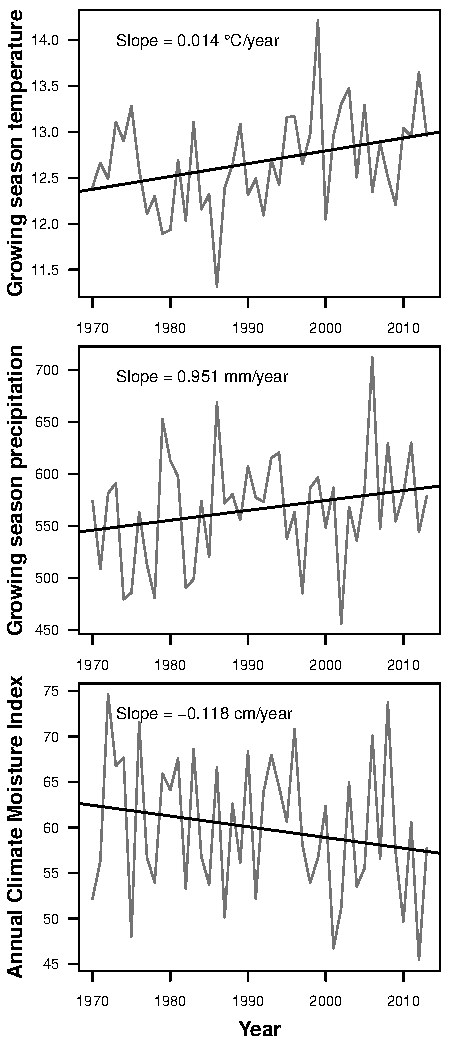
\includegraphics[width=3in,height=\textheight]{ms/figures/figS1_clim_trend.pdf}

\textbf{Figure S1}. Temporal trends in growing season temperatures
(top), total growing season precipitation (middle) and annual climate
moisture index (bottom). Grey lines represent averaged climate values
across the 6281 studied forest plots. Straight black lines show the
fitted least-squared linear regression lines.

\pagebreak

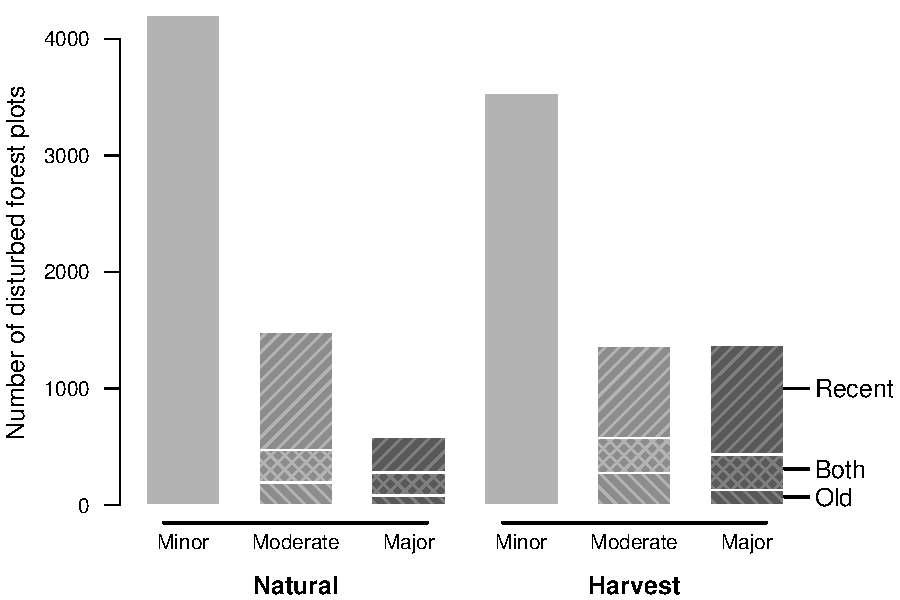
\includegraphics[width=4.5in,height=\textheight]{ms/figures/figS2_disturb.pdf}

\textbf{Figure S2}. Frequency of forest plots by disturbance type
(natural disturbances and harvest), level of intensity (minor, moderate,
major) and timing (old refers to disturbances that occurred before the
study period whereas recent disturbances occurred during the study
period). The three columns in each disturbance type sum to \emph{n} =
6281 forest plots, but many forest plots have been disturbed by more
than one type of disturbance during the study period.

\pagebreak

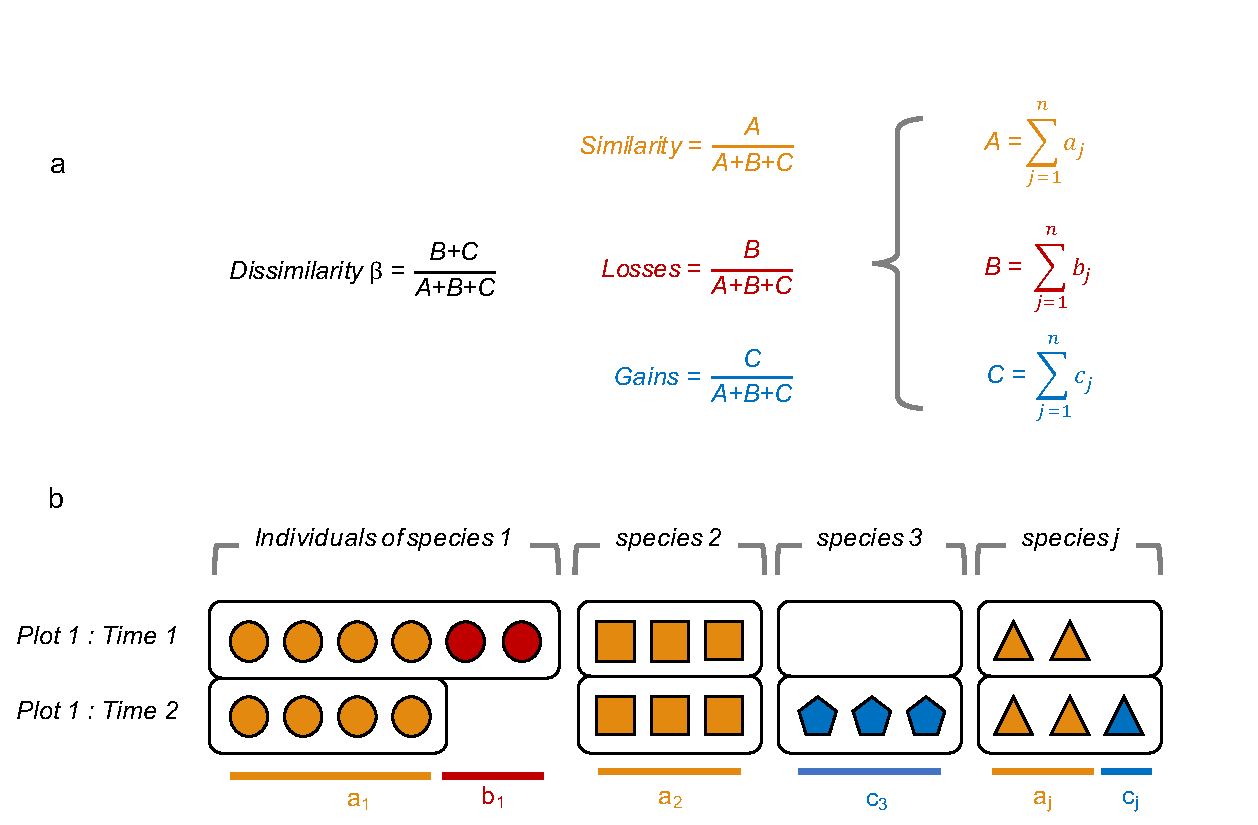
\includegraphics[width=6.6in,height=\textheight]{ms/figures/figS3_beta_calculus.pdf}

\textbf{Figure S3.} Equations to compute the temporal ß diversity index,
as well as its components, using the Ružička coefficient for abundance
data (a) and an example (b) where the tree composition of a single
forest plot is compared between two surveys, \(t_1\) and \(t_2\). In the
example, each of the \(n\) species is represented by a symbol. The
symbols in yellow represent the abundance of a species that is common to
the two survey (component A; note that it can be different individuals
of the same species). The symbols in red represent the abundance of a
species that is lost between \(t_1\) and \(t_2\) (component B). The
symbols in blue represent the abundance of a species that is gained
between \(t_1\) and \(t_2\) (component C). In this example,
\(A = 4 + 3 + 2 = 9\), \(B = 2\), and \(C = 3 + 1 = 4\), therefore
\(\beta = 2+4/(9+2+4) = 0.4\).

\pagebreak

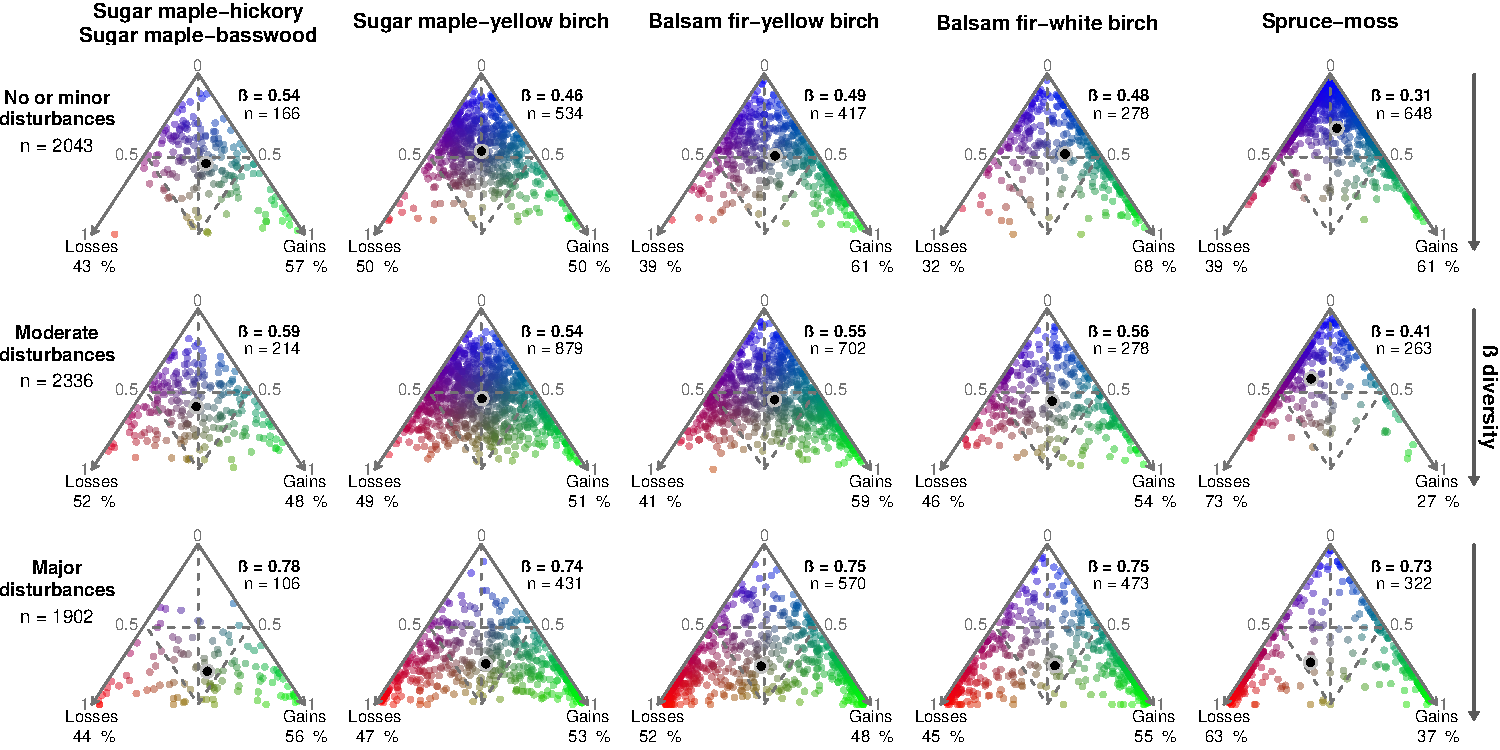
\includegraphics[width=6.6in,height=\textheight]{ms/figures/figS4_ternary.pdf}

\textbf{Figure S4}. Triangular diagrams of gains and losses in tree
abundance by bioclimatic domains and disturbance levels. Each point
represents a forest plot and the large black point represents the
centroid. At the upper tip of the triangle, similarity is high (ß = 0;
blue colors). At the base of the triangle, dissimilarity is high (ß =
1). On the left, forests in red are dominated by losses, while on the
right, forests in green are dominated by gains. The similar
distributions of gain and loss values in the ternary diagrams suggests
that there is no major difference in temporal ß diversity patterns among
domains.

\pagebreak

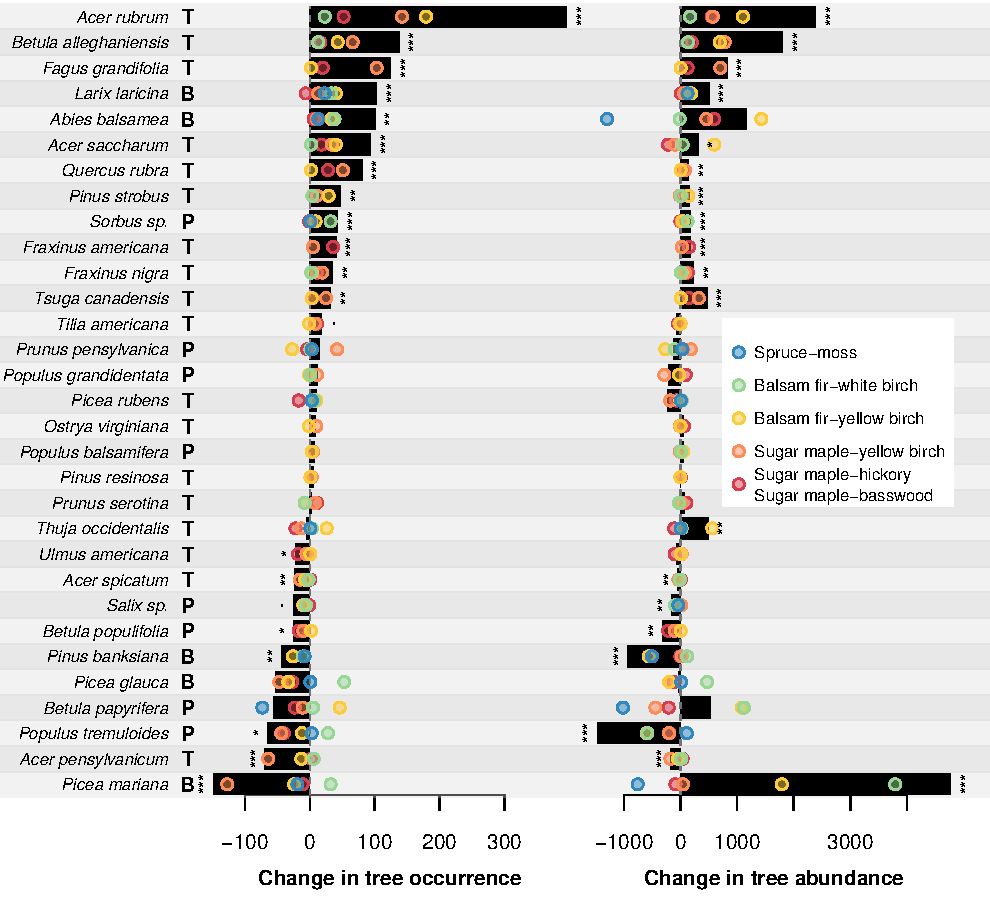
\includegraphics[width=6.6in,height=\textheight]{ms/figures/figS5_spchange.pdf}

\textbf{Figure S5.} Species temporal changes for Québec forests and for
each bioclimatic domain. Changes in species occurrence (left) and
species abundance (right). Only the species occupying more than 20 plots
are shown. The bars represent the mean changes across the study area,
while the colored points represent the mean changes by bioclimatic
domain. Stars represent the levels of the significance of the
\emph{p}-value (* \emph{p} \textless{} 0.05; ** \emph{p} \textless{}
0.01; *** \emph{p} \textless{} 0.001) associated with Wilcoxon
signed-rank tests used to determine whether individual species changes
in occurrence and abundance were significant. An increase in occurrence
indicates that the species has spread regionally, while an increase in
abundance indicates that the species has spread locally and/or
regionally. Letters next to species names correspond to (T)emperate;
(P)ioneer and (B)oreal species.

\pagebreak

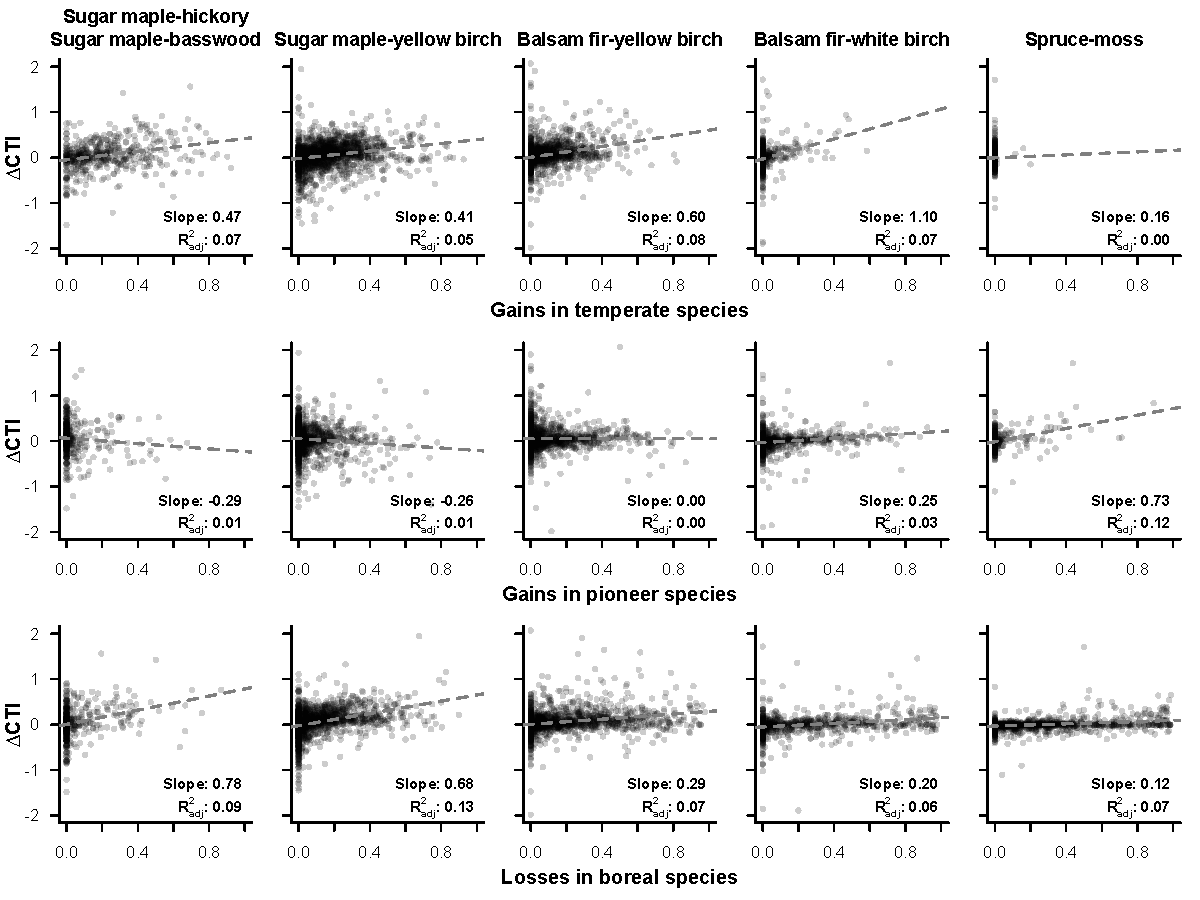
\includegraphics[width=6.6in,height=\textheight]{ms/figures/figS6_CTIvsGains.pdf}

\textbf{Figure S6.} Relations between change in Community Temperature
Index (\(\Delta\)CTI) and gains in temperate (top), gains in pioneer
(middle) and losses in boreal species (bottom). In each panel, the slope
and adjusted \(R^2\) of a linear regression model are shown.

\pagebreak

\hypertarget{references}{%
\section*{References}\label{references}}
\addcontentsline{toc}{section}{References}

\hypertarget{refs}{}
\leavevmode\hypertarget{ref-dray_adespatial_2018}{}%
Dray, S., Bauman, D., Blanchet, G., Borcard, D., Clappe, S., Guenard,
G., Jombart, T., Larocque, G., Legendre, P., Madi, N., \& Wagner, H. H.
(2018). \emph{Adespatial: Multivariate Multiscale Spatial Analysis}.
\url{https://CRAN.R-project.org/package=adespatial}

\leavevmode\hypertarget{ref-hijmans_raster_2018}{}%
Hijmans, R. J. (2018). \emph{Raster: Geographic Data Analysis and
Modeling}. \url{https://CRAN.R-project.org/package=raster}

\leavevmode\hypertarget{ref-laliberte_fd_2014}{}%
Laliberté, E., Legendre, P., \& Shipley, B. (2014). \emph{FD: Measuring
functional diversity from multiple traits, and other tools for
functional ecology}.

\leavevmode\hypertarget{ref-oksanen_vegan_2019}{}%
Oksanen, J., Blanchet, F. G., Friendly, M., Kindt, R., Legendre, P.,
McGlinn, D., Minchin, P. R., O'Hara, R. B., Simpson, G. L., Solymos, P.,
Stevens, M. H. H., Szoecs, E., \& Wagner, H. (2019). \emph{Vegan:
Community Ecology Package}.
\url{https://CRAN.R-project.org/package=vegan}

\leavevmode\hypertarget{ref-pebesma_simple_2018}{}%
Pebesma, E. (2018). Simple Features for R: Standardized Support for
Spatial Vector Data. \emph{The R Journal}.
\url{https://journal.r-project.org/archive/2018/RJ-2018-009/index.html}

\leavevmode\hypertarget{ref-r_core_team_r_2018}{}%
R Core Team. (2018). \emph{R: A Language and Environment for Statistical
Computing}. R Foundation for Statistical Computing.
\url{https://www.R-project.org/}

\leavevmode\hypertarget{ref-zeileis_zoo_2005}{}%
Zeileis, A., \& Grothendieck, G. (2005). Zoo: S3 Infrastructure for
Regular and Irregular Time Series. \emph{Journal of Statistical
Software}, \emph{14}(6), 1--27.
\url{https://doi.org/10.18637/jss.v014.i06}

\end{document}


%%%% Annexe article 2 %%%%



\renewcommand\thefigure{B.\arabic{figure}}
\renewcommand\thetable{B.\arabic{table}}

\include{article2/annexe2}

%%%% Annexe article 3 %%%%



\renewcommand\thefigure{C.\arabic{figure}}
\renewcommand\thetable{C.\arabic{table}}

\include{article3/annexe3}

\end{document}

\endinput
%%
%% End of file `gabaritTPA.tex'.
